\documentclass[lettersize,journal]{IEEEtran}
\usepackage[T1]{fontenc}
\usepackage[utf8]{inputenc}
\usepackage{amsmath,amsfonts,amsthm}
\usepackage{amssymb}
% \usepackage{algorithm}
% \usepackage{algpseudocode}
% \usepackage{algorithmic}
% \usepackage{algorithm}
\usepackage{algorithm}
\usepackage{algpseudocode}
\usepackage{array}
\usepackage[caption=false,font=normalsize,labelfont=sf,textfont=sf]{subfig}
\usepackage{textcomp}
\usepackage{stfloats}
\usepackage{xcolor,colortbl}
\definecolor{DarkGreen}{RGB}{1,50,32}
\usepackage{url}
\usepackage{verbatim}
\usepackage{graphicx}
\usepackage{cite}
% \PassOptionsToPackage{svgnames}{xcolor}
\hyphenation{op-tical net-works semi-conduc-tor IEEE-Xplore}
% updated with editorial comments 8/9/2021
\newtheorem{lemma}{Lemma}
% \newtheorem{problem}{Problem}
\newcommand{\problemtitle}[2]{%
  \parbox{\linewidth}{\centering\textbf{#1} \\ \textbf{#2}}%
}
\newtheorem{problem}{Problem}
\newtheorem{proposition}{Proposition}
\newtheorem{remark}{Remark}
\newtheorem{theorem}{\normalfont\textbf{Theorem}}
\newtheorem{corollary}{\normalfont\textbf{Corollary}}
\newcommand{\mycomment}[1]{}
\newcommand{\algrule}[1][.2pt]{\par\vskip.5\baselineskip\hrule height #1\par\vskip.5\baselineskip}
\newcolumntype{C}[1]{>{\centering\arraybackslash}p{#1}}
\newcolumntype{M}[1]{>{\centering\arraybackslash}m{#1}}
\let\labelindent\relax  % Redefine before loading enumitem
\usepackage{enumitem}
\newcommand{\purplecircle}{\textcolor{blue}{\textbullet}}
\newcommand{\largepurplecircle}{\textcolor{blue}{\scalebox{1.5}{$\bullet$}}}
\newcommand{\CRD}{$\text{C}_{\text{R}} \text{D }$}
\newcommand{\qedwhite}{\hfill \ensuremath{\Box}}
\newcommand{\algline}[1]{\begin{tabular}[t]{@{}l@{}}#1\end{tabular}}
% \usepackage{semantic}

\begin{document}

\title{Mathematical Comparison and Optimization of Urban Cycling Networks via Safety-Aware Clustering}

\author{Manuel Campero Jurado$^{1}$, Carlos Canudas-de-Wit$^{1}$, Giovanni De Nunzio$^{2}$% <-this % stops a space
% \thanks{*This work was not supported by any organization}% <-this % stops a space
%\thanks{We thank Dr.\ I.\ New for proofreading this paper. M.\ Campero Jurado visited Eindhoven University of Technology with the support of an outgoing mobility grant IDEX from the Univ.\ Grenoble Alpes.}
\thanks{$^{1}$Univ. Grenoble Alpes, Inria, CNRS, Grenoble INP, GIPSA-Lab, 38000 Grenoble, France
        {\footnotesize \{\textit{manuel.campero-jurado@inria.fr, carlos.canudas-de-wit@gipsa-lab.fr}\} }}%
\thanks{$^{2}$IFP Energies nouvelles,
Rond-point de l’échangeur de Solaize, BP 3, 69360 Solaize, France,
        {\footnotesize giovanni.de-nunzio@ifpen.fr}}%
}

% \author{IEEE Publication Technology,~\IEEEmembership{Staff,~IEEE,}
%         % <-this % stops a space
% \thanks{This paper was produced by the IEEE Publication Technology Group. They are in Piscataway, NJ.}% <-this % stops a space
% \thanks{Manuscript received April 19, 2021; revised August 16, 2021.}}

% % The paper headers
% \markboth{Journal of \LaTeX\ Class Files,~Vol.~14, No.~8, August~2021}%
% {Shell \MakeLowercase{\textit{et al.}}: A Sample Article Using IEEEtran.cls for IEEE Journals}

% \IEEEpubid{0000--0000/00\$00.00~\copyright~2021 IEEE}
% Remember, if you use this you must call \IEEEpubidadjcol in the second
% column for its text to clear the IEEEpubid mark.

\maketitle

\begin{abstract}
Comparing cycling networks across cities is challenging because networks differ in size, resolution, topology, and safety characteristics. Building on an existing exposure-based optimization model for cycling-infrastructure upgrades, this paper proposes a safety-aware framework for clustering, comparing, and transferring intervention strategies across urban cycling networks. Each network
is represented as a weighted directed graph whose arcs encode degree of separation, distance, cyclist flow, traffic exposure, slope, and angular change. We introduce a constrained clustering method that reduces large networks to a common resolution while preserving safety-relevant quantities such as exposure, flow, and DoS consistency. This enables fair cross-city comparison using an exposure-based Gromov--Wasserstein distance, and allows clustered optimization solutions to be lifted back to the original network. We further use the Gromov--Wasserstein correspondence to transfer optimized strategies from a source city to structurally similar target cities. A case study on Grenoble, Strasbourg, and Lyon shows that the clustered representation preserves optimization quality while reducing runtime, and that GW similarity provides an interpretable signal for cross-city transferability of cycling-infrastructure interventions.
\end{abstract}

\begin{IEEEkeywords}
Cycling networks, constrained clustering, cyclist exposure, bi-level optimization, urban mobility
\end{IEEEkeywords}

\section{Introduction}
\label{introduction}
The health, ecological, and socio-economic benefits of a cycling society are well-documented, including improved cardiovascular health, increased longevity, reduced carbon footprint and air pollution, lower transportation costs, reduced traffic congestion, and greater convenience and efficiency \cite{garrard2012health, gotschi2016cycling}. As a result, public authorities have made considerable efforts to promote cycling as an alternative to driving for short and medium distances. However, cyclists still face safety and comfort issues that may discourage them from riding \cite{fishman2012barriers}. It is well-established that infrastructure separating bicycles from motorized vehicles improves perceived safety and comfort, thereby encouraging higher cycling uptake \cite{lawrence2018cyclist, broach2012cyclists}. High-quality, well-connected cycling infrastructure can substantially increase ridership \cite{pucher2011walking, pucher2017cycling}. Yet, analyzing real-world cycling networks remains challenging due to their size, spatial complexity, and the many interacting factors that influence route choice and perceived safety. In addition, being able to compare the safety performance of different urban cycling networks in a fair and scale-independent way would be highly valuable for planners seeking to replicate successful strategies from cities with more advanced infrastructure.

\begin{figure}[t]
\centering
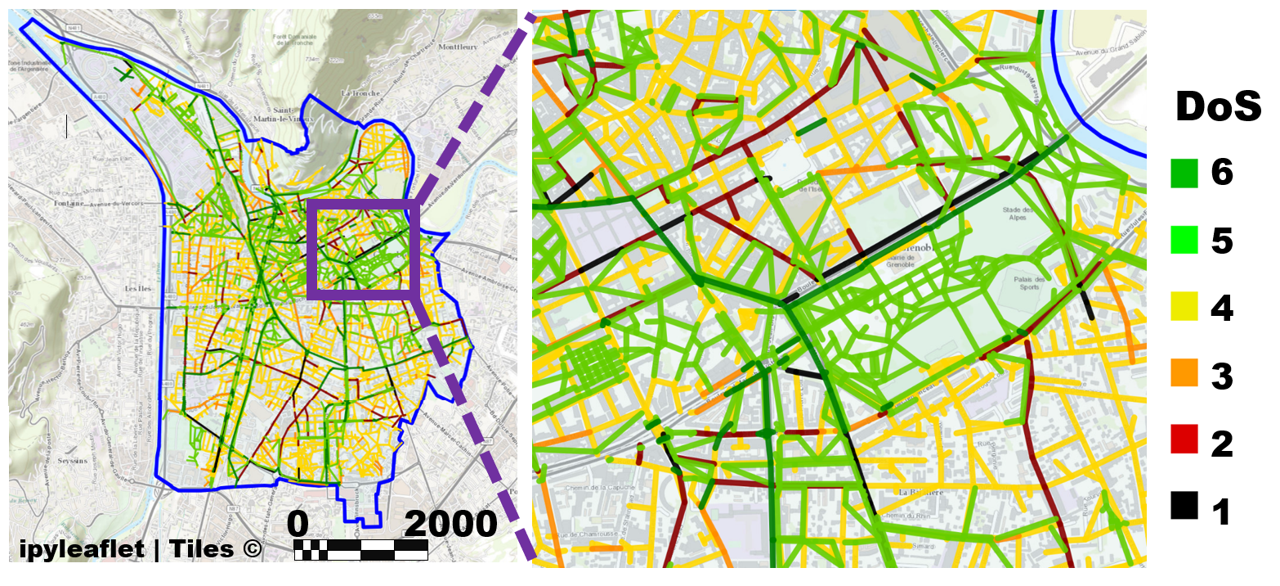
\includegraphics[width=1\columnwidth]{Images/map_scale.png}
\caption{\footnotesize Cycling network of Grenoble, France. The degree of separation (DoS) score of the cycling infrastructure from motorized vehicles is indicated in ascending order from 1 to 6.}
\label{networks_classification}
\end{figure}

% In this work, we propose a mathematical framework for fair comparison of cycling-network safety across cities with different sizes and levels of detail. Large road graphs are compressed into cluster-based supernetworks using a constrained k-means procedure applied to a safety-aware spectral embedding. This clustering preserves key safety attributes—including distance, slope, degree of separation from motor traffic, traffic factor, flow, and cyclist exposure—while explicitly limiting information loss. The algorithm progressively relaxes exposure and flow bounds while enforcing strict constraints on infrastructure type and spatial coherence, implemented via Lagrangian penalty terms in the k-means objective; when no feasible constrained solution exists, it safely reverts to standard k-means to ensure a valid clustering. On top of the clustered networks, we construct exposure-based kernels that encode how cyclist risk is distributed across the network. These kernels allow us to compare cities through structural similarity measures that capture both spatial patterns and safety-related attributes. Experiments on real cycling networks show that the clustered representations preserve safety-critical structure with high fidelity, enabling consistent and interpretable safety comparisons between cities of different sizes and network complexities.
We propose a mathematical framework to fairly compare cycling-network safety across cities of different sizes and detail levels. Large road graphs are compressed into cluster-based clustered-networks using a constrained, safety-aware k-means on a spectral embedding, preserving key attributes such as distance, slope, degree of separation, traffic factor, flow, and exposure while limiting information loss. On these clustered networks, we build exposure-based kernels to compare cities via structural similarity measures, and show on real cases that the clustered representations retain safety-critical structure well enough to enable consistent, interpretable cross-city safety comparisons.

% \textit{Related Work:} Our work draws on two primary domains: Transport network clustering or community detection and network comparison.

Related work: Our work is based on two main areas: transport network clustering or community detection and network comparison.

\textit{Community detection:} Cluster analysis and community detection are core tools for uncovering structure in complex data and networks. Classical $k$-means \cite{hartigan1979algorithm} partitions points into $K$ groups that minimize within-cluster variance, while network-specific methods identify densely connected node groups. Key approaches include edge-betweenness divisive methods \cite{girvan2002community}, greedy modularity maximization for large graphs \cite{clauset2004finding}, spectral algorithms based on the modularity matrix \cite{newman2006finding}, and fast physics-inspired methods using voltage-drop analogies \cite{wu2004finding}.

These generic techniques are widely used in transportation. In traffic-flow analysis, $k$-means has been applied to define flow phases from detector data \cite{xia2007defining}, detect disruptions on arterial networks \cite{gu2016unsupervised}, and characterize driving styles from automotive traces \cite{gace2021driving}. Hierarchical clustering has been used to derive recurrent daily profiles and distinguish workdays from weekends \cite{weijermars2005analyzing}. For spatially embedded transport networks, community detection supports homogeneous control regions and equity analysis: \cite{haghbayan2021community} use Infomap-based communities refined for homogeneity, contiguity, and compactness in perimeter control. In the cycling context, \cite{akbarzadeh2018designing} identify demand-based communities from taxi trips to design non-dominated bike networks, while \cite{natera2020data} propose data-driven, budget-aware strategies to connect fragmented bicycle networks. Bike-and-ride network design models further show how optimization can shift trips from private cars to bicycle–transit combinations \cite{tavassoli2020hub}. Compared with these works, our approach clusters cycling networks under explicit safety constraints so that the resulting clustered-networks preserve multi-attribute safety information and remain comparable across cities. To the best of our knowledge, existing clustering and community-detection methods are not explicitly designed to preserve cyclist-oriented safety indicators (e.g., exposure, slope, traffic conditions, angular change) when compressing large cycling networks for cross-city comparison.



\textit{Network comparison:} Comparing two transport networks can be seen as a relaxation of graph isomorphism: instead of asking whether a bijection makes their adjacencies identical, we ask how far apart their structures are under a chosen distance \cite{chartrand2013first}. A simple approach is to compare adjacency matrices via standard norms (Euclidean, Manhattan, etc.), in line with classical data analysis and data mining ideas \cite{hand2007principles}, but such measures are highly sensitive to node labelling and local perturbations.

More robust comparisons use structural descriptors. Global statistics such as clustering coefficient, diameter, and average path length provide coarse summaries, while higher-order pattern counts (graphlets) and role-based features capture finer functional similarity across complex networks \cite{yaverouglu2014revealing,faisal2017grafene}. Spectral methods use eigenvalues of adjacency or Laplacian matrices as label-invariant signatures, with spectral distances tracking graph edit distance in many cases \cite{wilson2008study}. From a more analytical viewpoint, cut distance and graphon theory offer limit objects and size-agnostic metrics with good empirical performance on diverse networks \cite{liu2018cut}. A complementary line embeds graphs into reproducing kernel Hilbert spaces via graph kernels. Early work defined positive definite kernels on labelled graphs despite the hardness of exact subgraph counting \cite{gartner2003graph}. Random-walk and marginalized kernels \cite{kashima2003marginalized,vishwanathan2010graph} exploit walk-based feature spaces while remaining computationally tractable, and are now standard tools for learning on graphs. All these approaches connect to optimal transport, which studies the most efficient way to redistribute mass. Wasserstein distances provide geometrically meaningful metrics between probability measures and have widespread applications in analysis and applied fields \cite{villani2008optimal,villani2021topics,santambrogio2015optimal}. In our setting, this viewpoint underlies how we compare exposure distributions and safety-relevant kernels on cycling networks, yielding a principled notion of “distance” between cities that is sensitive to both weights and structure. However, existing methods are rarely tailored to safety-specific attributes of cycling networks, nor do they jointly handle multi-attribute exposure measures and differences in network size or resolution when drawing cross-city conclusions. To the best of the authors' knowlarc, there is currently no framework that (i) clusters cycling networks under explicit safety constraints so as to preserve multi-attribute indicators such as flow, slope, and angular change, and (ii) compares the resulting networks in a size-independent and mathematically consistent way using exposure-based kernels.

\textit{Statement of Contribution}: We propose a safety-aware framework for cross-city cycling-network analysis that:
(i) models cyclist exposure using DoS, flow, traffic, distance, slope, and
angular-change information; (ii) formulates original and clustered bi-level
upgrade problems for reducing exposure under a budget; (iii) introduces a
constrained clustering-and-lifting strategy that preserves safety-relevant
network structure while reducing computational cost; and (iv) uses an
exposure-based Gromov--Wasserstein (GW) distance to compare cities and transfer
optimized infrastructure strategies between structurally similar networks.
Experiments on Grenoble, Strasbourg, and Lyon show that the clustered approach
closely approximates direct optimization and that GW similarity provides a useful
basis for transferability.





\section{Model Design}
\label{model_design}
In this section, we first present the bike lane classification and the graph representation. We then define the cyclist flow model and the
traffic-exposure measure on the original network. Next, we extend these
quantities to the clustered representation, so that flow, exposure, and
safety-relevant attributes are preserved after aggregation. Finally, we present
the safety-aware clustering algorithm used to construct reduced networks that
remain comparable across cities.



\begin{table}[t]
\centering
\vspace{0.2cm}
\begin{tabular}{|c|p{5cm}|c|}
\hline
\textbf{DoS}   & \textbf{Description} & \textbf{AADT (veh/day)} \\
\hline
$6$  & Dedicated bike lanes, fully separated from motor traffic. & 14 400 \\

$5$  & Bike lanes shared with pedestrians, separate from cars. & 16 000 \\ 

$4$  & Mixed-traffic roads (30 km/h) without designated bike lanes. & 960  \\

$3$  & Shared roads with cycling pictograms. & 3 120 \\

$2$  & Roads with painted bike lanes.  & 6 912 \\

$1$  & Unmarked shared car-bike lanes. & 8 448 \\
\hline
\end{tabular}
\caption{\footnotesize The degree of separation (DoS) categorizes bike lane infrastructure based on safety levels. The third column presents annual average daily traffic (AADT) on adjacent roads, sourced from the GTLVille platform in Grenoble \cite{gtlville2024}.}
\label{dos_table}
\end{table}
\subsection{Bike Lane  Safety classification}


The DoS classification, adapted from an OSM-based platform, categorizes cycling infrastructure based on separation from motor traffic. Table~\ref{dos_table} presents DoS categories, showing that higher-DoS lanes offer greater safety. These scores serve as weights in the network graph, modeling upgrades from lower to higher safety levels. The classification methodology is detailed in \cite{2024graphbased}. Fig.~\ref{networks_classification} visualizes these classifications in the Grenoble cycling network.



\subsection{Graph Representation}


Let the network be represented by a weighted directed graph (digraph) $\mathcal{G} = (\mathcal{V}, \mathcal{A}, \mathcal{W})$, where $\mathcal{V}$ is the set of nodes corresponding to intersections or road endpoints, $\mathcal{A}$ is the set of directed arcs representing roads, and $\mathcal{W}$ is the set of weights assigned to those arcs. For each arc $a = (u, v) \in \mathcal{A}$, with $u,v \in \mathcal{V}$, the original weight $w_a^{0} \in \mathcal{W}$ represents the DoS associated with the link. The weights are assumed to be symmetric, meaning $w_{(u,v)}^{0} = w_{(v,u)}^{0}$. The geographical length of each arc $a$ is denoted by $d_a$.

\subsection{Cyclist Flows}
\label{section_flows}

Following \cite{mesbah2012bilevel}, we use an all-or-nothing (AON) traffic assignment model that assumes no congestion and assigns all demand $q_{(u,v)}$ from the EMD2020 survey \cite{SMMAG_EMD} to the shortest available path  between nodes $u,v \in \mathcal{V}$. This reflects typical cycling dynamics, where congestion effects are minimal. In this section, we formalize and adopt the cyclist distance proposed in \cite{cooper2017using}, which defines this distance using OpenStreetMap and Cardiff cycling flow data while incorporating infrastructure characteristics. Then, betweenness centrality is applied to estimate the flow distribution.

To account for cycling-specific factors, we use a modified distance metric that accounts for key factors influencing route choice. Let $\mathcal{V}$ denote the set of nodes in the network, and let $u, v \in \mathcal{V}$ be two nodes. The shortest path between $u$ and $v$ is represented as $p_{(u,v)} = (a_{1},\ldots, a_{k})$, where each arc $a~\in~p_{(u,v)}$ has a geographical length $d_{a}$, an angular change $\measuredangle_a$ (in degrees, either along $a$ or at junctions between consecutive arcs), a slope factor $s_{a}$ (which depends on the terrain slope $m_{a}$), and a traffic factor $f_{a}$ (that takes into account the flow of car traffic on roads adjacent to bike lanes). We define the cyclist distance $b_{(u,v)}$ between nodes $u$ and $v$ as

\begin{equation}
\label{cyclist_distance}
    b_{(u,v)} = \sum_{a \in p_{(u,v)}} \left( d_a \cdot s_a \cdot (f_a)^{\rho} \right) +  \sum_{a \in p_{(u,v)}} \measuredangle_a \cdot \eta,
\end{equation}
where $\rho > 0$ and $\eta > 0$ are calibration parameters controlling the influence of traffic conditions and angular changes, respectively.
The traffic factor $f_a$ is defined as
\begin{equation}
\label{f_a}
f_a(w_{a}^{0}) = 
     \begin{cases}
\psi \cdot \exp{\left( \phi^{\text{AADT}}_{a} \right)} & \text{if } w_{a}^{0} < 5, \\
\psi \cdot 2.03 & \text{if } w_{a}^{0} = 5, \\
\psi & \text{if } w_{a}^{0} = 6.
\end{cases}
\end{equation}

Here, $\phi^{\text{AADT}}_{a}$ represents the annual average daily traffic (AADT) of the adjacent car lanes, expressed in thousands. The variable $w_{a}^{0}$ denotes the original DoS of the bike lane $a$. According to \cite{cyclerap2024}, the impact of annual average daily traffic (AADT) is neutralized when $w_{a}^{0} \geq 5$, indicating full separation from car lanes. The factor 2.03 accounts for an observed increase in crash risk in shared spaces with pedestrians compared to separate, exclusive bicycle lanes \cite{mesimaki2021near}. The parameter $\psi$ is a scaling factor.  
Let $p_{(u,v)}$ be the shortest path between nodes $u$ and $v$ based on the cyclist distance in Eq.~\eqref{cyclist_distance}. Since the origin-destination (OD) demand in our data is symmetric, each node acts as both an origin and a destination, ensuring balanced inflow and outflow. The flow conservation for paths is given by
\begin{equation}
\label{eq_shortest_path}
    \phi_{p_{(u,v)}} = q_{(u,v)},
\end{equation}
where $q_{(u,v)}$ represents the demand between nodes $u$ and $v$.  
Next, let $\mathbb{I}_{a \in p_{(u,v)}}$ be a binary variable indicating whether arc $a$ is part of the shortest path $p_{(u,v)}$. Then, the total cyclist flow on arc $a$, denoted as $\phi_a$, is
\begin{equation}
\begin{aligned}
\label{eq_flows}
  & \phi_{a}  = \sum_{u,v \in \mathcal{V}} q_{(u,v)} \cdot \mathbb{I}_{a \in p_{(u,v)}} \geq 0, \quad \forall a \in \mathcal{A}  \\
  & \Phi  = \sum_{a \in \mathcal{A}} \phi_{a}.
\end{aligned}
\end{equation}
This ensures that the total flow on each arc is the sum of all demands for trips passing through it, maintaining balance across the network due to the symmetry of the demand matrix. To assess cyclist exposure to traffic conditions, we introduce $\mathcal{E}$ as a general measure of exposure, defined for pahts in the network. This metric helps evaluate network improvements. For a shortest path $p_{(u,v)} = (a_1, \dots, a_k)$, cyclist exposure captures the combined effect of traffic-related risk and the distance of cyclist interaction with traffic, and is defined as
\begin{equation}
\label{exposure_def}
    \mathcal{E}_{p_{(u,v)}} = \sum_{a \in p_{(u,v)}} d_{a} \cdot f_{a} \cdot \phi_{a},
\end{equation}
where $\phi_{a}, d_{a}$ and $f_{a}$ are the normalized arc flow, length and traffic factor, respectively. For a single arc $a \in \mathcal{A}$, cyclist exposure simplifies to
\begin{equation}
\label{arc_exposure}
    \mathcal{E}_{a} = d_{a} \cdot f_{a} \cdot \phi_{a} \in  \left [ 0,1 \right ].
\end{equation}

Then, for the original network the total cyclist exposure is:
\begin{equation}
    \mathcal{E}^{\text{orig}} = \frac{1}{|\mathcal{A}|} \sum_{(v_{i},v_{j}) \in \mathcal{A}} \phi_{(v_{i},v_{j})} \cdot f(w_{(v_{i},v_{j})}) \cdot d_{(v_{i},v_{j})}.
\end{equation}
Having presented the graph representation, cyclist flow model, and exposure-based safety indicator, we now turn to the clustering algorithm. The purpose of this step is to construct a reduced network that preserves the safety-relevant attributes introduced above, including flow, traffic exposure, slope, angular change, and infrastructure quality. This clustered representation provides the basis for comparing and optimizing cycling networks across cities in a fair and scale-independent manner.
%%%%%%%%%%%%%%%%%%%%%%%%%%%%%%%%%%%%%%%%%%%%%%%%%%%%%%%%%%%%%%%%%%%%%%%%%%%%%%%%%%%%%%%%%%%%%%%%%%%%%%%%%%



\subsection{Cluster Network Definition}

Let $\mathcal{P}=\{C_1,\dots,C_k\}$ be a partition of the node set $\mathcal{V}$ into
$k$ non-empty clusters. We define the clustered network as
$\tilde{\mathcal{G}}=(\tilde{\mathcal{V}},\tilde{\mathcal{A}},\tilde{\mathcal{W}})$,
where each cluster becomes a clustered-node, i.e.,
$\tilde{\mathcal{V}}=\mathcal{P}$.

For any pair of clusters $(C_r,C_{r'})$, let
\[
  \mathcal{A}(C_r,C_{r'})
  =
  \bigl\{(u,v)\in\mathcal{A}\mid u\in C_r,\; v\in C_{r'}\bigr\}
\]
denote the set of original arcs connecting them. A clustered-arc
$\tilde{a}=(C_r,C_{r'})$ is included in $\tilde{\mathcal{A}}$ whenever
$\mathcal{A}(C_r,C_{r'})\neq\varnothing$. For notational simplicity, intra-cluster
arcs are denoted by
\[
  \mathcal{A}(C_r):=\mathcal{A}(C_r,C_r).
\]

The clustered DoS weights are defined conservatively using the minimum DoS among
the underlying arcs. Thus, for $r~\neq ~r'$,
\begin{equation}
  \tilde{w}^{\mathrm{inter}}_{(C_r,C_{r'})}
  =
  \min_{a\in\mathcal{A}(C_r,C_{r'})} w_a,
\end{equation}
while the intra-cluster DoS weight is
\begin{equation}
  \tilde{w}^{\mathrm{intra}}_{C_r}
  =
  \min_{a\in\mathcal{A}(C_r)} w_a.
\end{equation}
These definitions preserve the highest-risk connection between or within clusters.



\subsection{Clustered cyclist distance}


To aggregate arc-level attributes in the clustered cycling network, we use flow-weighted averages. For any arc
attribute $x_a$ and any non-empty arc set $S\subseteq\mathcal{A}$, define
\begin{equation}
  \langle x\rangle_S^\phi
  :=
  \frac{\sum_{a\in S} x_a\, \cdot \phi_a}
       {\sum_{a\in S} \phi_a},
\end{equation}
whenever $\sum_{a\in S}\phi_a>0$. This choice gives greater importance to arcs
that carry larger cyclist flows.

Let $\tilde{p}_{(C_r,C_{r'})}=(\tilde{a}_1,\dots,\tilde{a}_m)$ denote a shortest
path between clusters $C_r$ and $C_{r'}$ in $\tilde{\mathcal{G}}$, and let
$\mathcal{C}(C_r,C_{r'})\subseteq\tilde{\mathcal{V}}$ be the set of clusters
visited along this path. The clustered cyclist distance is defined as
\begin{equation}
\label{eq:clustered_cyclist_distance}
  \tilde{b}_{(C_r,C_{r'})}
  =
  \sum_{\tilde{a}\in\tilde{p}_{(C_r,C_{r'})}}
  \tilde{b}^{\mathrm{inter}}_{\tilde{a}}
  +
  \sum_{C_q\in\mathcal{C}(C_r,C_{r'})}
  \tilde{b}^{\mathrm{intra}}_{C_q}.
\end{equation}
For an inter-cluster clustered-arc $\tilde{a}=(C_r,C_{r'})$, with $r\neq r'$, we set
\begin{equation}
  \tilde{b}^{\mathrm{inter}}_{\tilde{a}}
  =
  \tilde{d}^{\mathrm{inter}}_{\tilde{a}} \cdot
  \tilde{s}^{\mathrm{inter}}_{\tilde{a}} \cdot
  \bigl(\tilde{f}^{\mathrm{inter}}_{\tilde{a}}\bigr)^\rho
  +
  \tilde{\measuredangle}^{\mathrm{inter}}_{\tilde{a}} \cdot \eta,
\end{equation}
where
\begin{equation}
\begin{aligned}
  \tilde{d}^{\mathrm{inter}}_{\tilde{a}}
  &= \langle d\rangle_{\mathcal{A}(C_r,C_{r'})}^{\phi}, \qquad
  \tilde{s}^{\mathrm{inter}}_{\tilde{a}}
  = \langle s\rangle_{\mathcal{A}(C_r,C_{r'})}^{\phi}, \\
  \tilde{\measuredangle}^{\mathrm{inter}}_{\tilde{a}}
  &= \langle \measuredangle\rangle_{\mathcal{A}(C_r,C_{r'})}^{\phi}, \qquad
  \tilde{f}^{\mathrm{inter}}_{\tilde{a}}
  = f\bigl(\tilde{w}^{\mathrm{inter}}_{(C_r,C_{r'})}\bigr).
\end{aligned}
\end{equation}
Similarly, the intra-cluster contribution of cluster $C_r$ is
\begin{equation}
  \tilde{b}^{\mathrm{intra}}_{C_r}
  =
  \tilde{d}^{\mathrm{intra}}_{C_r} \cdot
  \tilde{s}^{\mathrm{intra}}_{C_r} \cdot
  \bigl(\tilde{f}^{\mathrm{intra}}_{C_r}\bigr)^\rho
  +
  \tilde{\measuredangle}^{\mathrm{intra}}_{C_r} \cdot \eta,
\end{equation}
with
\begin{equation}
\begin{aligned}
\label{eq:clustered_parameters}
  \tilde{d}^{\mathrm{intra}}_{C_r}
  &= \langle d\rangle_{\mathcal{A}(C_r)}^{\phi}, \qquad \quad
  \tilde{s}^{\mathrm{intra}}_{C_r}
  = \langle s\rangle_{\mathcal{A}(C_r)}^{\phi}, \\
  \tilde{\measuredangle}^{\mathrm{intra}}_{C_r}
  &= \langle \measuredangle\rangle_{\mathcal{A}(C_r)}^{\phi}, \qquad \quad
  \tilde{f}^{\mathrm{intra}}_{C_r}
  = f\bigl(\tilde{w}^{\mathrm{intra}}_{C_r}\bigr).
\end{aligned}
\end{equation}


\subsection{Clustered demand, flow assignment, and exposure}

Given the original network $\mathcal{G}$ and its clustered representation
$\tilde{\mathcal{G}}$, the clustered demand between two clusters is obtained by
aggregating all original OD demands with origins in the first cluster and
destinations in the second:
\begin{equation}
\label{cluster_demand}
  \tilde{q}_{(C_r,C_{r'})}
  :=
  \sum_{\substack{u\in C_r \\ v\in C_{r'}}}
  q_{(u,v)}.
\end{equation}
For the all-or-nothing assignment on the clustered graph, let
$\tilde{p}_{(C_r,C_{r'})}$ be the shortest path between $C_r$ and $C_{r'}$
computed using the clustered cyclist distance in
\eqref{eq:clustered_cyclist_distance}. The inter-cluster flow on a clustered-arc
$\tilde{a}\in\tilde{\mathcal{A}}$ is
\begin{equation}
\label{eq_cluster_flow_inter}
  \tilde{\phi}^{\mathrm{inter}}_{\tilde{a}}
  :=
  \sum_{r,r'}
  \tilde{q}_{(C_r,C_{r'})} \cdot
  \mathbb{I}_{\tilde{a}\in\tilde{p}_{(C_r,C_{r'})}}.
\end{equation}

Similarly, the intra-cluster flow associated with $C_q$ is the total clustered
demand whose shortest path visits that cluster:
\begin{equation}
\label{eq_cluster_flow_intra}
  \tilde{\phi}^{\mathrm{intra}}_{C_q}
  :=
  \sum_{r,r'}
  \tilde{q}_{(C_r,C_{r'})} \cdot
  \mathbb{I}_{C_q\in\mathcal{C}(C_r,C_{r'})}.
\end{equation}
The clustered total exposure is then defined as the average exposure over
inter-cluster clustered-arcs and intra-cluster components:
\begin{equation}
\label{eq_cluster_total_exposure}
  \mathcal{E}^{\mathrm{clust}}
  :=
  \frac{
    \mathcal{E}^{\mathrm{inter}}+\mathcal{E}^{\mathrm{intra}}
  }{
    |\tilde{\mathcal{A}}|+k
  },
\end{equation}
where
\begin{equation}
\label{cluster_def}
\begin{aligned}
  \mathcal{E}^{\mathrm{inter}}
  &:=
  \sum_{\tilde{a}\in\tilde{\mathcal{A}}}
  \tilde{\phi}^{\mathrm{inter}}_{\tilde{a}} \cdot
  \tilde{f}^{\mathrm{inter}}_{\tilde{a}}
  \cdot \tilde{d}^{\mathrm{inter}}_{\tilde{a}}, \\
  \mathcal{E}^{\mathrm{intra}}
  &:=
  \sum_{r=1}^{k}
  \tilde{\phi}^{\mathrm{intra}}_{C_r}
  \cdot
  \tilde{f}^{\mathrm{intra}}_{C_r}
  \cdot
  \tilde{d}^{\mathrm{intra}}_{C_r}.
\end{aligned}
\end{equation}
The corresponding total clustered flow is
\begin{equation}
  \Phi^{\mathrm{clust}}
  :=
  \sum_{\tilde{a}\in\tilde{\mathcal{A}}}
  \tilde{\phi}^{\mathrm{inter}}_{\tilde{a}}
  +
  \sum_{r=1}^{k}
  \tilde{\phi}^{\mathrm{intra}}_{C_r}.
\end{equation}

% %%%%%%%%%%%%%%%%%%%%%%%%%%%%%%






\begin{figure*}[h!]
\vspace{0.2cm}
  \centering
  \captionsetup[subfigure]{font={footnotesize}, labelfont={footnotesize, bf}, textfont={footnotesize, rm}}

  \subfloat[Original]{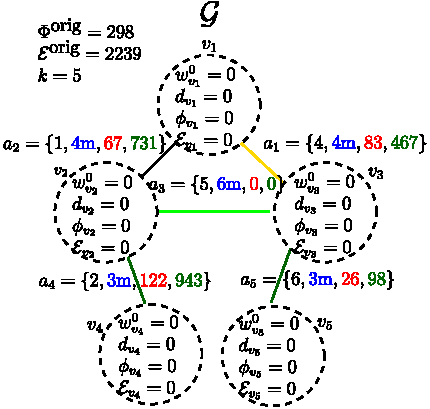
\includegraphics[width=0.24\linewidth]{Images/G.pdf}\label{fig::ae_orig}}
  \hspace{0.001\linewidth}
  % \hspace{0.001\linewidth} % Adjust horizontal space as needed
  \subfloat[Cluster $k=4$]
  {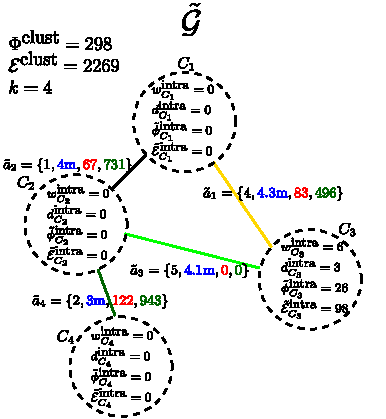
\includegraphics[width=0.24\linewidth]{Images/G_4.pdf}\label{fig::ae_4}} 
  \hspace{0.001\linewidth} % Adjust horizontal space as needed
  \subfloat[Cluster $k=3$]{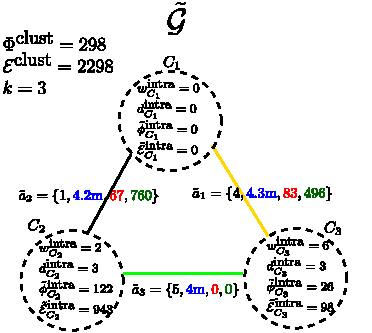
\includegraphics[width=0.24\linewidth]{Images/G_3.pdf}\label{fig::ae_3}}
  \hspace{0.001\linewidth} % Adjust vertical space as needed
  \subfloat[Cluster $k=2$]{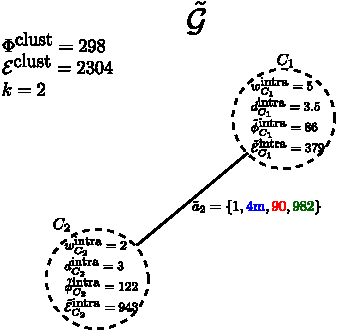
\includegraphics[width=0.24\linewidth]{Images/G_2.pdf}\label{fig::ae_2}}
  \caption{\footnotesize Algorithm 1 for toy example where $a~=~\left \{w_{a}^{0} , \textcolor{blue}{d_{a} (\mbox{m})}, \textcolor{red}{\phi_{a}}, \textcolor{DarkGreen}{\mathcal{E}_{a}} \right \}$, $\tilde{a}^{\mbox{inter}}~=~\left \{w^{\mbox{inter}}_{\tilde{a}} , \textcolor{blue}{d^{\mbox{inter}}_{\tilde{a}} (\mbox{m})}, \textcolor{red}{\phi^{\mbox{inter}}_{\tilde{a}}}, \textcolor{DarkGreen}{\mathcal{E}^{\mbox{inter}}_{\tilde{a}}} \right \}$, and $C^{\mbox{intra}}~=~\left \{d^{\mbox{intra}}_{C} , \textcolor{blue}{d^{\mbox{intra}}_{C} (\mbox{m})}, \textcolor{red}{\phi^{\mbox{inter}}_{C}}, \textcolor{DarkGreen}{\mathcal{E}^{\mbox{intra}}_{C}} \right \}$}
  \label{fig:ae_clustering}
\end{figure*}



\subsection{Clustering Algorithm (CC)}

One of our objectives is to compare cycling networks of different sizes, then, we cluster the larger network until its number of clustered-nodes matches the number of nodes in the smaller network. The goal is to construct a reduced graph $\tilde{\mathcal{G}}$ that remains faithful to the original network in terms of safety-relevant attributes, including DoS, distance, slope, traffic factor, cyclist flow, and exposure.

We first define a safety-aware weighted adjacency matrix:
\begin{equation}
\label{eq:adjacency_matrix}
A_{ij} =
\begin{cases}
w_{ij}^{0}\,\cdot \exp\!\left(-\dfrac{d_{ij}}{\gamma}\right)\cdot 
\left(\dfrac{\phi_{ij}}{\max \phi}\right)^{\alpha},
& \text{if } (i,j)\in\mathcal{A},\\[0.6em]
0, & \text{otherwise},
\end{cases}
\end{equation}
where $w_{ij}^{0}$ is the DoS value, $d_{ij}$ is the spatial distance, $\phi_{ij}$ is the cyclist flow on arc $(i,j)$, $\gamma>0$ controls the effect of spatial proximity, and $\alpha\geq0$ controls the importance of high-flow arcs. The corresponding normalized Laplacian is
\begin{equation}
\label{eq:modified_laplacian}
  \mathcal{L}=I-D^{-1/2}AD^{-1/2},
  \qquad
  D_{ii}=\sum_j A_{ij}.    
\end{equation}
A spectral embedding is obtained from $\mathcal{L}$, and clustering is then performed in this embedded space. The clustering step uses a constrained $k$-means procedure, summarized in Algorithm~\ref{alg:constrained-clustering-math} and detailed in Appendix~A and this clustered constrained algorithm will be called CC-Algorithm. The constraints are designed to preserve both local safety consistency and global network-level quantities. Specifically, the algorithm uses the following parameters:
\[
\epsilon_{\max},\quad
\delta_{\max},\quad
\tau_{\mathcal{E}}^{(0)},\quad
\tau_{\Phi}^{(0)},\quad
\alpha_{\mathrm{relax}}.
\]
Here, $\epsilon_{\max}$ bounds the allowed DoS variation inside each cluster, while $\delta_{\max}$ limits the spatial diameter of a cluster. The initial tolerances
\[
\tau_{\mathcal{E}}^{(0)}
=
\frac{\left|\mathcal{E}^{\mathrm{clust}}-\mathcal{E}^{\mathrm{orig}}\right|}
{\mathcal{E}^{\mathrm{orig}}},
\qquad
\tau_{\Phi}^{(0)}
=
\frac{\left|\Phi^{\mathrm{clust}}-\Phi^{\mathrm{orig}}\right|}
{\Phi^{\mathrm{orig}}},
\]
control the admissible relative distortion in total exposure and total flow, respectively. The parameter $\alpha_{\mathrm{relax}}>1$ gradually relaxes these tolerances if no feasible clustering is found.

At each iteration, the algorithm applies $k$-means in the spectral embedding
while penalizing violations of the exposure and flow constraints. DoS
homogeneity and spatial compactness are enforced as hard constraints. If no
feasible clustering is found, the exposure and flow tolerances are gradually
relaxed; if the problem remains infeasible, the method falls back to standard
spectral $k$-means. This ensures that a clustered network
$\tilde{\mathcal{G}}$ is always obtained, while preserving the main safety and
flow characteristics of the original graph. Fig.~\ref{fig:ae_clustering}
illustrates the clustering procedure on a toy example. The constrained clustering procedure admits the following theoretical guarantees.

\begin{theorem}[Legitimacy of the normalized Laplacian]
\label{thm:symmetry}
The matrix $\mathcal{L}=I-D^{-1/2}AD^{-1/2}$ is a valid symmetric normalized graph Laplacian.
\end{theorem}


\begin{theorem}[Flow Preservation in Network Clustering]
\label{thm:flow_preservation}
Given a di-graph $\mathcal{G} = (\mathcal{V}, \mathcal{A}, \mathcal{W})$ with demand matrix $q_{(u,v)}$ and its clustered representation $\tilde{\mathcal{G}} = (\tilde{\mathcal{V}}, \tilde{\mathcal{A}}, \tilde{\mathcal{W}})$ constructed via Algorithm~\ref{alg:constrained-clustering-math}, the total network flow is preserved:
\[
\Phi^{\text{orig}} \triangleq \sum_{a \in \mathcal{A}} \phi_a
= \sum_{\tilde{a} \in \tilde{\mathcal{A}}} \tilde{\phi}_{\tilde{a}}
= \Phi^{\text{clust}}.
\]
\end{theorem}

\begin{proof}
The proofs are provided in Appendix~A.
\end{proof}



%%%%%%%%%%%%%%%%%%%%%%%%%%%%%%%%%%%%%%%%%%%%%%%%%%%%%%%%%%


We now formulate the infrastructure-upgrade problem. First, we present the original arc-level bi-level model, where upgrades are assigned to individual arcs. Then, we derive a clustered counterpart that reduces computational complexity while preserving the main exposure and routing effects.


\section{Optimization Framework}
\label{sec:optimization_framework}

After defining the exposure measures and clustered representation, we formulate
the infrastructure-upgrade problem. The goal is to decide which cycling links
should be improved, and to what DoS level, under a fixed budget. Because
upgrades affect route choice, we model the problem as a bi-level optimization:
the upper level selects infrastructure upgrades, while the lower level recomputes
cyclist flows through an all-or-nothing assignment. We first present the
arc-level formulation and then introduce a clustered version that reduces
computational complexity while preserving the interaction between upgrades,
routing, and exposure.


\subsection{Original Arc-Level Optimization Problem}
\label{subsec:original_optimization}



% Given a fixed budget $B$, our objective is to improve cycling infrastructure by upgrading the DoS on selected road segments, the optimization problem has two interconnected levels. The upper-level problem $\mathbb{U}_{\mathrm{pper}}$
% represents the strategic infrastructure-planning decision. It chooses which arcs
% to upgrade, and to what DoS level, in order to minimize total cyclist exposure
% to motorized traffic while satisfying a budget constraint. The objective combines
% arc length, traffic factor, and cyclist flow, so that long, highly used, and
% high-exposure arcs are prioritized.

% The lower-level problem $\mathbb{L}_{\mathrm{ower}}$ represents cyclists' route choice after the upgrades have
% been implemented. For each OD pair, cyclists are assigned to the shortest path
% with respect to the upgraded cyclist distance, using the all-or-nothing
% assignment introduced in Section~\ref{section_flows}. Since changes in the DoS
% at the upper level modify the traffic factors and cyclist distances, they also
% affect the lower-level flow distribution. Therefore, the two levels are nested.
Given a fixed budget $B$, we model infrastructure upgrading as a bi-level
optimization problem as in \cite{jurado2025improving}. The upper level $\mathbb{U}_{\mathrm{pper}}$ selects which arcs to upgrade and to what
DoS level, with the goal of minimizing total cyclist exposure under the budget
constraint. The lower level $\mathbb{L}_{\mathrm{ower}}$ then recomputes cyclists' route choices using the
AON assignment with the upgraded cyclist distances. Since DoS changes affect
traffic factors, shortest paths, and flows, the two levels are coupled.

We define the following notation:
\begin{itemize}
    \item $\mathbf{w}^{0} = \left [  w_{a}^{0} \right ]_{a \in \mathcal{A}}^\top \in \mathbb{N}^{|\mathcal{A}|}$: vector of original DoS values for each arc in the bike network;
    \item $\mathbf{w} = \left [   w_{a} \right ]_{a \in \mathcal{A}}^\top \in \Omega$: vector of decision variables (candidate configuration) representing the upgraded DoS values, where $\Omega$ is the constraint set that defined as 
$\Omega
=
\left\{
\mathbf{w}\in
\mathbb{N}^{|\mathcal{A}|}
:
w_a^{0}
\leq
w_a
\leq
6,\quad
\forall a\in\mathcal{A}
\right\}$;
% \item $\phi_{a}(\tilde{\mathbf{w}}) \in \mathbb{R}_{\geq 0}$: Flow on arc $a \in \mathcal{A}$;
% \item $d_{a} \in \mathbb{R}_{\geq 0}$:  Length of $a \in \mathcal{A}$; 
% \item $\bar{d}_{a} \in \mathbb{R}_{\geq 0}$: Cyclist distance of $a \in \mathcal{A}$;
\item $\pi(w_{a}^{0},w_{a})  \in \mathbb{R}_{\geq 0}$: the cost or price per meter of upgrading arc $a$ from $w_{a}^{0}$ to $w_{a}$. 
\end{itemize}
The original arc-level bi-level optimization problem is then written as follows:
\begin{problem}{Original bi-level network-upgrade optimization problem}\label{bi-levelorig}
\begin{align}
& \mathbb{U}_{\mathrm{pper}}: \nonumber \\[0.2em]
& \mathbf{w}^{\star}
=
\arg\min_{\mathbf{w}\in\Omega}
\;
\frac{1}{|\mathcal{A}|}\sum_{a\in\mathcal{A}}
\phi_a^{\star}(\mathbf{w})
\cdot
f_a(w_a)
\cdot
d_a
\label{eq:upper_arc}
\\
& \quad \quad  \mathrm{s.t. }
\sum_{a\in\mathcal{A}}
d_a
\cdot
\pi(w_a^{0},w_a)
\leq B,
\label{eq:budget_arc}
\\[0.5em]
& \quad \quad \mathbb{L}_{\mathrm{ower}}: \nonumber \\[0.2em]
& \quad \quad
\boldsymbol{\phi}^{\star}
(\boldsymbol{w})
=
\arg\min_{\boldsymbol{\phi}\in
\mathbb{R}_{\geq 0}^{|\mathcal{A}|}}
\;
\sum_{a\in\mathcal{A}}
\bar{d}_a(\mathbf{w})
\cdot
\phi_a,
\label{eq:lower_arc}
\\
& \quad \quad 
\mathrm{s.t.}\,
\phi_a
=
\sum_{(u,v)\in
\mathcal{V}_{\mathcal{O}}
\times
\mathcal{V}_{\mathcal{D}}}
q_{(u,v)}
\cdot
\mathbb{I}_{
a\in p_{(u,v)}
(\mathbf{w})
}
\geq 0,
\quad
\forall a\in\mathcal{A}.
\nonumber
\end{align}
\end{problem}
Then $\mathbf{w}^{\star}$ denotes the solution of Problem~\ref{bi-levelorig}.

\subsection{Cluster-Level Optimization}
\label{subsec:cluster_optimization}

Solving the original bi-level problem directly on $\mathcal{G}$ can be
computationally demanding, since the upper level contains one decision variable
for each arc in $\mathcal{A}$. We therefore formulate a clustered counterpart on
the aggregated network $\tilde{\mathcal{G}}$, defined in the previous section.

The clustered model makes upgrade decisions on aggregated objects rather than on
individual arcs. Let
\[
\mathcal{G}_{\mathrm{agg}}
=
\tilde{\mathcal{V}}
\cup
\tilde{\mathcal{A}}
\]
denote the set of upgradeable objects, where elements of $\tilde{\mathcal{V}}$
represent intra-cluster infrastructure and elements of $\tilde{\mathcal{A}}$
represent inter-cluster connections. Thus, upgrading a cluster $C_r$ applies to
the original arcs in $\mathcal{A}(C_r)$, while upgrading a clustered-arc
$(C_r,C_s)$ applies to the original arcs in $\mathcal{A}(C_r,C_s)$.

For each object $g\in\mathcal{G}_{\mathrm{agg}}$, let $w_g^0$ be its initial DoS
level, defined using the conservative clustered DoS weights:
\[
w_g^0
=
\begin{cases}
\tilde{w}^{\mathrm{intra}}_{C_r},
& \text{if } g=C_r\in\tilde{\mathcal{V}},\\[0.3em]
\tilde{w}^{\mathrm{inter}}_{(C_r,C_s)},
& \text{if } g=(C_r,C_s)\in\tilde{\mathcal{A}}.
\end{cases}
\]
The clustered upgrade decision is $\tilde{\mathbf{w}}
= \left [\tilde{w}_g\right ]_{g\in\mathcal{G}_{\mathrm{agg}}} \in \mathbb{N}^{|\mathcal{G}_{\mathrm{agg}}|}$, where $\tilde{w}_g$ is the upgraded DoS level of object $g$. The feasible set is
\begin{equation}
\label{eq:Omega_cluster_conf}
\tilde{\Omega}
=
\left\{
\tilde{\mathbf{w}}\in
\mathbb{N}^{|\mathcal{G}_{\mathrm{agg}}|}
:
w_g^0
\leq
\tilde{w}_g
\leq
6,
\quad
\forall g\in\mathcal{G}_{\mathrm{agg}}
\right\}.
\end{equation}

As in the arc-level formulation, the upgraded DoS determines the traffic factor.
For each $g\in\mathcal{G}_{\mathrm{agg}}$, we define
\begin{equation}
\label{eq:cluster_traffic_factor_conf}
f_g(\tilde{w}_g)
=
\begin{cases}
\psi \cdot \exp(\phi_g^{\mathrm{AADT}}), & \tilde{w}_g < 5,\\
2.03\, \cdot \psi, & \tilde{w}_g = 5,\\
\psi, & \tilde{w}_g = 6,
\end{cases}
\end{equation}
where $\phi_g^{\mathrm{AADT}}$ is the aggregated AADT value associated with object
$g$.

Given an upgrade vector $\tilde{\mathbf{w}}$, the clustered cyclist distance is
computed as in Eq.~\eqref{eq:clustered_cyclist_distance}, replacing the baseline
traffic factors by the upgraded factors $f_g(\tilde{w}_g)$. For each clustered OD
pair $(C_r,C_s)$, let
$\tilde{p}_{(C_r,C_s)}(\tilde{\mathbf{w}})$ denote the resulting shortest path in
$\tilde{\mathcal{G}}$. Given the clustered demand $\tilde{q}_{(C_r,C_s)}$, the lower-level
all-or-nothing assignment sends all demand between $C_r$ and $C_s$ to
$\tilde{p}_{(C_r,C_s)}(\tilde{\mathbf{w}})$. The induced inter-cluster $\tilde{\phi}^{\mathrm{inter}}_{\tilde{a}}(\tilde{\mathbf{w}})$ and intra-cluster $\tilde{\phi}^{\mathrm{intra}}_{C_q}(\tilde{\mathbf{w}})$
flows are defined as Eq. \eqref{eq_cluster_flow_inter}-\eqref{eq_cluster_flow_intra}, respectively. Using the aggregated distances already defined in the clustered cyclist-distance
formulation, the total clustered exposure under $\tilde{\mathbf{w}}$ is denoted by $\mathcal{E}^{\mathrm{clust}}(\tilde{\mathbf{w}})$ and defined as in Eq. \eqref{eq_cluster_total_exposure}.

For each clustered upgradeable object
$g\in\mathcal{G}_{\mathrm{agg}}$, let $\mathcal{A}(g)$ be the set of original
arcs represented by $g$:
\[
\mathcal{A}(g)
=
\begin{cases}
\mathcal{A}(C_r),
& \text{if } g=C_r\in\tilde{\mathcal{V}}, \\[0.4em]
\mathcal{A}(C_r,C_s),
& \text{if } g=(C_r,C_s)\in\tilde{\mathcal{A}}.
\end{cases}
\]
Since $w_g^0$ is defined as the minimum DoS among the arcs in
$\mathcal{A}(g)$, an upgraded value $\tilde{w}_g$ is interpreted as a minimum
target DoS for all arcs represented by $g$. Hence, only arcs with
$w_a^0<\tilde{w}_g$ are upgraded, while arcs already satisfying
$w_a^0\geq\tilde{w}_g$ remain unchanged.

The cost of upgrading object $g$ is therefore
\begin{equation}
\label{eq:cluster_upgrade_cost_exact}
\Pi_g(\tilde{w}_g)
=
\sum_{a\in\mathcal{A}(g)}
d_a\, \cdot
\pi
\left(
w_a^0,
\max\{w_a^0,\tilde{w}_g\}
\right),
\end{equation}
where $d_a$ is the arc length and $\pi(\cdot,\cdot)$ is the unit cost per meter
of the corresponding DoS upgrade and arcs that already have DoS greater than or equal to $\tilde{w}_g$ are left unchanged. The clustered bi-level network-upgrade problem is then
\begin{problem}{Clustered bi-level network-upgrade optimization problem}
\label{bi-levelcluster}
\begin{align}
& \mathbb{U}_{\mathrm{pper}}: \nonumber \\[0.2em]
& \tilde{\mathbf{w}}^{\star}
=
\arg\min_{\tilde{\mathbf{w}}\in\tilde{\Omega}}
\;
\mathcal{E}^{\mathrm{clust}}(\tilde{\mathbf{w}})
\label{eq:cluster_bi-level_upper_conf}
\\
& \quad \quad \mathrm{s.t. }
\sum_{g\in\mathcal{G}_{\mathrm{agg}}}
\Pi_g(\tilde{w}_g)
\leq B.
\label{eq:cluster_bi-level_budget_conf}
\\[0.5em]
& \quad \quad \mathbb{L}_{\mathrm{ower}}: \nonumber \\[0.2em]
& \quad \quad
\tilde{\boldsymbol{\phi}}^{\star}(\tilde{\mathbf{w}})
\text{ satisfies the AON assignment induced by Eq. \eqref{eq:clustered_cyclist_distance}}.
\nonumber
\end{align}
\end{problem}

Problem~\ref{bi-levelcluster} is the clustered counterpart of
Problem~\ref{bi-levelorig}. It optimizes DoS upgrades on aggregated objects
under a budget constraint, while recomputing cyclist flows on the clustered
network. The solution $\tilde{\mathbf{w}}^{\star}$ can then be lifted back to
the original graph, providing a computationally lighter approximation that still
captures the interaction between upgrades, route choice, and exposure.


\section{Network Comparison}
\label{sec:gw_comparison}



The purpose of this work is to compare the safety structure of two cycling networks
of different sizes. Let $\mathcal{H}=(\mathcal{V}^\mathcal{H},\mathcal{A}^\mathcal{H},\mathcal{W}^\mathcal{H})$
be the smaller network, and let $\mathcal{G}$ be the larger network. We cluster
$\mathcal{G}$ into
$\tilde{\mathcal{G}}=(\tilde{\mathcal{V}}^{\mathcal{G}},\tilde{\mathcal{A}}^{\mathcal{G}},\tilde{\mathcal{W}}^{\mathcal{G}})$,
where $\tilde{\mathcal{V}}^{\mathcal{G}}=\mathcal{C}=\{C_1,\dots,C_k\}$, such that
\[
    |\mathcal{V}(\mathcal{H})|
    =
    |\tilde{\mathcal{V}}^{\mathcal{G}}|
    =
    k .
\]
This size matching allows the two networks to be compared at the same resolution.
In what follows, superscripts $\mathcal{H}$ and $\tilde{\mathcal{G}}$ indicate the
network to which each quantity belongs.


We compare the two networks using a Gromov--Wasserstein (GW) distance based on
their internal exposure structure. For each directed arc $(i,j)\in\mathcal{A}(\mathcal{H})$,
we define the arc exposure as
\begin{equation}
    \mathcal{E}^{\mathcal{H}}_{ij}
    =
    \phi^{\mathcal{H}}_{ij} \cdot
    f^{\mathcal{H}}_{ij} \cdot
    d^{\mathcal{H}}_{ij},
\end{equation}
where $\phi^{\mathcal{H}}_{ij}$ is the cyclist flow, $f^{\mathcal{H}}_{ij}$ is the traffic
factor, and $d^{\mathcal{H}}_{ij}$ is the arc length. The exposure mass assigned to
node $v_i\in\mathcal{V}(\mathcal{H})$ is the total exposure of its incident arcs:
\begin{equation}
    \mu^{\mathcal{H}}(v_i)
    =
    \sum_{(i,j)\in\mathcal{A}(\mathcal{H})}
    \mathcal{E}^{\mathcal{H}}_{ij}
    +
    \sum_{(j,i)\in\mathcal{A}(\mathcal{H})}
    \mathcal{E}^{\mathcal{H}}_{ji}.
\end{equation}

Analogously, for each super-arc $(C_r,C_s)\in\tilde{\mathcal{A}}^{\mathcal{G}}$, we define
\begin{equation}
    \tilde{\mathcal{E}}^{\tilde{\mathcal{G}}}_{rs}
    =
    \tilde{\phi}^{\mathrm{inter}}_{rs} \cdot
    \tilde{f}^{\mathrm{inter}}_{rs} \cdot
    \tilde{d}^{\mathrm{inter}}_{rs},
\end{equation}
where $\tilde{\phi}^{\mathrm{inter}}_{rs}$ is the inter-cluster flow,
$\tilde{f}^{\mathrm{inter}}_{rs}$ is the inter-cluster traffic factor, and
$\tilde{d}^{\mathrm{inter}}_{rs}$ is the flow-weighted inter-cluster distance. The exposure mass of a clustered node $C_r\in\tilde{\mathcal{V}}^{\mathcal{G}}$ is
defined by adding incoming, outgoing, and intra-cluster exposure:
\begin{equation}
    \mu^{\tilde{\mathcal{G}}}(C_r)
    =
    \sum_{(C_r,C_s)\in\tilde{\mathcal{A}}^{\mathcal{G}}}
    \tilde{\mathcal{E}}^{\tilde{\mathcal{G}}}_{rs}
    +
    \sum_{(C_s,C_r)\in\tilde{\mathcal{A}}^{\mathcal{G}}}
     \left ( \tilde{\mathcal{E}}^{\tilde{\mathcal{G}}}_{sr}
    +
    \tilde{\mathcal{E}}^{\mathrm{intra}}_{C_r} \right ).
\end{equation}
The node masses are normalized into probability measures:
\begin{equation}
    \hat{\mu}^{\mathcal{H}}(v_i)
    =
    \frac{\mu^{\mathcal{H}}(v_i)}
    {\sum_{u\in\mathcal{V}(\mathcal{H})}\mu^{\mathcal{H}}(u)},
    \quad
    \hat{\mu}^{\tilde{\mathcal{G}}}(C_r)
    =
    \frac{\mu^{\tilde{\mathcal{G}}}(C_r)}
    {\sum_{s=1}^{k}\mu^{\tilde{\mathcal{G}}}(C_s)}.
\end{equation}
These probability measures describe how cyclist exposure is distributed across
the nodes of each network. To compare the internal structure of these exposure distributions, we define
pairwise dissimilarity matrices for both networks. Let $x_i\in\mathbb{R}^2$ be
the geographical coordinates of node $v_i\in\mathcal{V}(\mathcal{H})$, and let
$c_r\in\mathbb{R}^2$ be the centroid of cluster $C_r$. We set
\begin{equation}
    D^{\mathcal{H}}_{ij}
    =
    \left|
        \hat{\mu}^{\mathcal{H}}(v_i)
        -
        \hat{\mu}^{\mathcal{H}}(v_j)
    \right|
    +
    \gamma
    \|x_i-x_j\|_2,
    \quad
    i,j=1,\dots,k,
\end{equation}
and
\begin{equation}
    D^{\tilde{\mathcal{G}}}_{rs}
    =
    \left|
        \hat{\mu}^{\tilde{\mathcal{G}}}(C_r)
        -
        \hat{\mu}^{\tilde{\mathcal{G}}}(C_s)
    \right|
    +
    \gamma
    \|c_r-c_s\|_2,
    \quad
    r,s=1,\dots,k.
\end{equation}
Here, $\gamma>0$ balances exposure dissimilarity and geographical separation.

Let $\mathrm{T}(\hat{\mu}^{\mathcal{H}},\hat{\mu}^{\tilde{\mathcal{G}}})$ be the set of admissible
transport couplings between the two probability measures:

\begin{equation}
\begin{aligned}
    \mathrm{T}(\hat{\mu}^{\mathcal{H}},\hat{\mu}^{\tilde{\mathcal{G}}})
    =
    \Bigl\{
    \mathrm{t}\in\mathbb{R}_{+}^{k\times k}
    \;\Big|\;&
    \sum_{s=1}^{k}\mathrm{t}_{is}
    =
    \hat{\mu}^{\mathcal{H}}(v_i),
    \quad i=1,\dots,k,\\
    &
    \sum_{i=1}^{k}\mathrm{t}_{is}
    =
    \hat{\mu}^{\tilde{\mathcal{G}}}(C_s),
    \quad s=1,\dots,k
    \Bigr\}.
\end{aligned}
\end{equation}
The squared Gromov--Wasserstein distance is then
\begin{equation}
\label{eq:gw_definition}
    \mathrm{t}^{\star}(\mathcal{H},\tilde{\mathcal{G}})
    = \sqrt{
    \min_{\mathrm{t}\in\mathrm{T}(\hat{\mu}^{\mathcal{H}},\hat{\mu}^{\tilde{\mathcal{G}}})}
    \sum_{i,j=1}^{k}
    \sum_{r,s=1}^{k}
    \left(
        D^{\mathcal{H}}_{ij}
        -
        D^{\tilde{\mathcal{G}}}_{rs}
    \right)^2
    \mathrm{t}_{ir}
    \mathrm{t}_{js}.}
\end{equation}
A small value of $\mathrm{t}^{\star}(\mathcal{H},\tilde{\mathcal{G}})$ indicates that the two
networks have similar internal exposure structures. In particular, it means that
high-exposure and spatially important regions in the smaller network can be
matched to analogous regions in the clustered larger network, without requiring
a predefined node-to-node correspondence.
\section{Optimization Transfer Through Network Comparison}
\label{sec:optimization_transfer}

The previous sections introduced the two components that enable cross-city
transfer: a clustered representation that puts networks at a common resolution,
and a GW distance that measures similarity between their exposure-weighted
structures. We now use the corresponding GW transport plan to investigate
whether an upgrade strategy optimized on a source network can be transferred to
a target network. In this way, the comparison step is used not only to measure
similarity, but also to guide infrastructure interventions across cities.

We consider three complementary steps. First, each network is optimized
independently under a common relative budget. Second, for clustered networks, we
compare clustered optimization with original arc-level optimization after lifting
the clustered solution back to the original graph. Third, we transfer an
optimized upgrade pattern from a source network to a target network using the GW
transport plan.

\subsection{Clustered Versus Original Optimization}
\label{subsec:clustered_vs_original_optimization}

For a network $\mathcal{G}$ and its clustered representation
$\tilde{\mathcal{G}}$, we compare the original arc-level optimization with the
cluster-level approximation. The original strategy is obtained by solving
Problem~\ref{bi-levelorig} on the full graph, yielding $\mathbf{w}^{\star}
~=~\left[
w_a^{\star}
\right]_{a\in\mathcal{A}}^{\top}
\in
\mathbb{N}^{|\mathcal{A}|}$.
The clustered strategy is obtained by solving Problem~\ref{bi-levelcluster} on
the aggregated graph, yielding
$
\tilde{\mathbf{w}}^{\star}~=~\left[
\tilde{w}_g^{\star}
\right]_{g\in\mathcal{G}_{\mathrm{agg}}}^{\top}~\in~\mathbb{N}^{|\mathcal{G}_{\mathrm{agg}}|}.
$

Because the initial DoS of a clustered object $g$ is defined as the minimum DoS
among its underlying arcs, the clustered decision
$\tilde{w}_g^{\star}$ is interpreted as a minimum target safety
level for all arcs represented by $g$. Therefore, when lifting the clustered
solution back to the original graph, an arc is upgraded only if its original DoS
is below the optimized clustered DoS. For every
$a\in\mathcal{A}(g)$, we define
\begin{equation}
\label{eq:lifted_cluster_solution}
w_a^{\star,\mathrm{lift}}
=
\max
\left\{
w_a,
\tilde{w}_g^{\star}
\right\}.
\end{equation}
Thus, arcs that are less safe than the clustered target are upgraded to
$\tilde{w}_g^{\star}$, while arcs that already have DoS greater
than or equal to this value remain unchanged. The lifted vector is denoted by $\mathbf{w}^{\star,\mathrm{lift}}
=
\left[
w_a^{\star,\mathrm{lift}}
\right]_{a\in\mathcal{A}}^{\top}$. The lifted strategy is then evaluated on the original network by recomputing the
cyclist distances, the all-or-nothing assignment, and the total exposure
$\mathcal{E}^{\mathrm{orig}}(\mathbf{w}^{\star,\mathrm{lift}})$.

% We measure the quality of the clustered approximation using the lifting
% efficiency
% \begin{equation}
% \rho_{\mathrm{lift}}
% =
% \frac{
% \mathcal{E}^{\mathrm{orig}}(\mathbf{w})
% -
% \mathcal{E}^{\mathrm{orig}}(\mathbf{w}^{\star,\mathrm{lift}})
% }{
% \mathcal{E}^{\mathrm{orig}}(\mathbf{w})
% -
% \mathcal{E}^{\mathrm{orig}}(\mathbf{w}^{\star})
% }.
% \end{equation}
% A value close to one indicates that the lifted clustered solution achieves a
% similar exposure reduction to the original arc-level optimum when both are
% evaluated on the full network.

\subsection{GW-Based Transfer of Upgrade Strategies}
\label{subsec:gw_transfer}





We now use the GW correspondence to construct an approximate solution of
Problem~\ref{bi-levelorig} on the target network $\mathcal{G}$. Instead of
solving the full arc-level problem directly on $\mathcal{G}$, we transfer an
optimized strategy from a source network $\mathcal{H}$ whose safety-exposure
structure is similar to that of the clustered target network
$\tilde{\mathcal{G}}$. This similarity is measured by a small value of
$GW(\mathcal{H},\tilde{\mathcal{G}})$.

Following the clustering procedure introduced above, $\mathcal{G}$ is first
reduced to
\[
\tilde{\mathcal{G}}
=
(\tilde{\mathcal{V}}^{\mathcal{G}},
 \tilde{\mathcal{A}}^{\mathcal{G}},
 \tilde{\mathcal{W}}^{\mathcal{G}})
\]
such that
\[
|\tilde{\mathcal{V}}^{\mathcal{G}}|
=
|\mathcal{V}^{\mathcal{H}}|.
\]
This gives both networks the same resolution. Let $\mathrm{t}^{\star}$ denote
the optimal GW transport plan between $\mathcal{H}$ and
$\tilde{\mathcal{G}}$, as defined in Section~\ref{sec:gw_comparison}.

\begin{figure*}[ht]
    \centering
    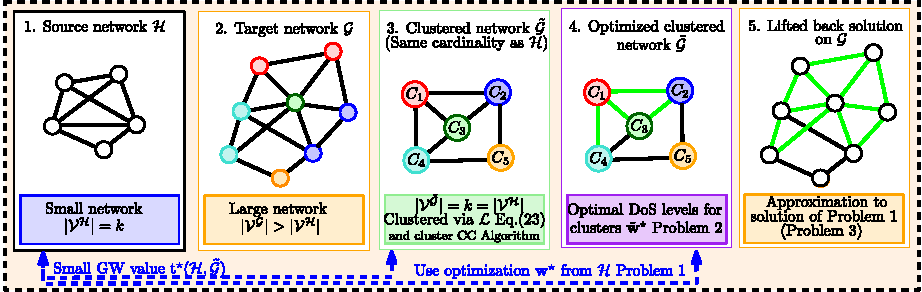
\includegraphics[width=2\columnwidth]{Images/25_05_2026_clustering.pdf}\\

    \caption{Overview of the transfer framework: the target network $\mathcal{G}$ is
clustered to match the source network $\mathcal{H}$; the optimized strategy
from $\mathcal{H}$ is transferred to $\tilde{\mathcal{G}}$ and then lifted back
to $\mathcal{G}$ as an approximate arc-level solution.}
    \label{fig:framework_explanation}
\end{figure*}

Assume that the source network $\mathcal{H}$, with baseline DoS vector
$\mathbf{w}^{0,\mathcal{H}}
=
\left[
w_a^{0,\mathcal{H}}
\right]_{a\in\mathcal{A}^{\mathcal{H}}}^{\top}
\in
\mathbb{N}^{|\mathcal{A}^{\mathcal{H}}|},$
has been optimized under budget $B^{\mathcal{H}}$, yielding $\mathbf{w}^{\star,\mathcal{H}}
~=~
\left[
w_a^{\star,\mathcal{H}}
\right]_{a\in\mathcal{A}^{\mathcal{H}}}^{\top}
\in
\mathbb{N}^{|\mathcal{A}^{\mathcal{H}}|}.$
We summarize the source upgrade around each node
$v_i\in\mathcal{V}^{\mathcal{H}}$ by
\begin{equation}
\label{eq:source_upgrade_intensity}
u_i^{\mathcal{H}}
=
\frac{
\sum_{a\in\mathcal{N}^{\mathcal{H}}(i)}
\mathcal{E}_a^{\mathcal{H}}(\mathbf{w}^{\mathcal{H}})
\cdot
\left(
w_a^{\star,\mathcal{H}}
-
w_a^{0,\mathcal{H}}
\right)
}{
\sum_{a\in\mathcal{N}^{\mathcal{H}}(i)}
\mathcal{E}_a^{\mathcal{H}}(\mathbf{w}^{\mathcal{H}})
+
\varepsilon
},
\end{equation}
where $\mathcal{N}^{\mathcal{H}}(i)$ is the set of arcs incident to node $i$,
$\mathcal{E}_a^{\mathcal{H}}(\mathbf{w}^{\mathcal{H}})$ is the baseline exposure
of arc $a$, and $\varepsilon>0$ avoids division by zero. Thus,
$u_i^{\mathcal{H}}$ is large when highly exposed arcs around node $i$ receive
large DoS improvements in the optimized source solution.

The GW plan $\mathrm{t}^{\star}$ transfers the source upgrade intensities to the
clustered target network. For each cluster
$C_r\in\tilde{\mathcal{V}}^{\mathcal{G}}$, we define
\begin{equation}
\label{eq:target_transfer_score_cluster}
u_{C_r}^{\mathcal{H}\rightarrow\tilde{\mathcal{G}}}
=
\frac{
\sum_i
\mathrm{t}_{ir}^{\star}
\cdot
u_i^{\mathcal{H}}
}{
\sum_i
\mathrm{t}_{ir}^{\star}
+
\varepsilon
}.
\end{equation}
The value $u_{C_r}^{\mathcal{H}\rightarrow\tilde{\mathcal{G}}}$ is the
transferred upgrade score of cluster $C_r$. It is a weighted average of the
source upgrade intensities $u_i^{\mathcal{H}}$, where the weights are given by
the GW coupling $\mathrm{t}_{ir}^{\star}$. Therefore, this score is large when
cluster $C_r$ is strongly matched to source nodes that were strongly upgraded in
the optimized solution on $\mathcal{H}$.

We then assign a priority score $S_g$ to each upgradeable object
$g\in\mathcal{G}_{\mathrm{agg}}^{\tilde{\mathcal{G}}}$. If $g$ is an
intra-cluster object, its score is the transferred score of that cluster. If
$g$ is an inter-cluster object, its score is the average transferred score of
the two endpoint clusters:
\begin{equation}
\label{eq:object_priority_score}
S_g
=
\begin{cases}
u_{C_r}^{\mathcal{H}\rightarrow\tilde{\mathcal{G}}},
& \text{if } g=C_r, \\[0.5em]
\dfrac{
u_{C_r}^{\mathcal{H}\rightarrow\tilde{\mathcal{G}}}
+
u_{C_s}^{\mathcal{H}\rightarrow\tilde{\mathcal{G}}}
}{2},
& \text{if } g=(C_r,C_s).
\end{cases}
\end{equation}
Thus, $S_g$ measures how important object $g$ is according to the upgrade
pattern transferred from $\mathcal{H}$.

The transferred clustered strategy is obtained by maximizing the total priority
of the selected upgrades under the target budget. Let
\[
\tilde{\mathbf{w}}
=
\left[
\tilde{w}_g
\right]_{g\in\mathcal{G}_{\mathrm{agg}}^{\tilde{\mathcal{G}}}}^{\top}
\in
\tilde{\Omega}^{\tilde{\mathcal{G}}}
\]
be a candidate DoS vector on the clustered target network. The objective rewards
assigning higher DoS levels to clustered objects with larger transferred
priority scores.

\begin{problem}{GW-based transferred clustered upgrade problem}
\label{prob:gw_transfer_clustered}
\begin{align}
\tilde{\mathbf{w}}^{\star,\mathrm{trans},\tilde{\mathcal{G}}}
=
\arg\max_{\tilde{\mathbf{w}}\in\tilde{\Omega}^{\tilde{\mathcal{G}}}}
&
\sum_{g\in\mathcal{G}_{\mathrm{agg}}^{\tilde{\mathcal{G}}}}
S_g
\cdot
\tilde{w}_g
\label{eq:transfer_projection_clustered}
\\
\mathrm{s.t.}\quad
&
\sum_{g\in\mathcal{G}_{\mathrm{agg}}^{\tilde{\mathcal{G}}}}
\Pi_g(\tilde{w}_g)
\leq
B^{\mathcal{G}}.
\label{eq:transfer_projection_budget_clustered}
\end{align}
\end{problem}

Here, $S_g$ is the transferred priority score of object $g$,
$\tilde{w}_g$ is the DoS assigned to $g$, $\Pi_g(\tilde{w}_g)$ is the aggregated cost
of raising the original arcs represented by $g$ to at least $\tilde{w}_g$, and
$B^{\mathcal{G}}$ is the available budget for the target network.

Problem~\ref{prob:gw_transfer_clustered} is a budgeted projection of the source
solution onto $\tilde{\mathcal{G}}$. It does not solve the full bi-level
Problem~\ref{bi-levelorig} on $\mathcal{G}$ directly. Instead, it uses the GW
transport plan to identify which clustered objects of the target network should
receive higher safety levels, based on the optimized intervention pattern of the
source network, Fig.~\ref{fig:framework_explanation} shows a summary of the whole framework.

\section{Solution Algorithms}
\label{sec:solution_algorithms}

The proposed problems are discrete bi-level network-design problems, where the
upper level selects integer DoS upgrades and the lower level recomputes cyclist
flows through AON assignment. Since related formulations are NP-hard
\cite{jurado2025graph}, we use genetic algorithms to approximate both the
arc-level and clustered problems. Each candidate DoS vector is evaluated by
updating traffic factors, recomputing routes and flows, and using the resulting
exposure as fitness; budget-infeasible candidates are repaired or penalized. The
corresponding pseudo-codes are provided in Appendix~B.
% The optimization problems introduced above are discrete bi-level network-design
% problems. In particular, the upper level chooses integer DoS values, while the
% lower level recomputes cyclist route choices through an all-or-nothing
% assignment. Related network-design formulations are known to be NP-hard
% \cite{jurado2025graph}. Therefore, instead of seeking exact solutions, we
% use genetic algorithms (GAs) to obtain high-quality approximate solutions for
% both the original arc-level problem and its clustered counterpart.

% The general idea is the same in both cases. A candidate solution is represented
% by a vector of DoS values. For each candidate, the corresponding traffic factors
% and cyclist distances are updated, the lower-level AON assignment is recomputed,
% and the resulting exposure is used as the fitness value. Candidate solutions
% that violate the budget constraint are repaired or penalized, and all pseudo-codes of this section are presented in Appendix~B.

\subsection{GA for the Original Arc-Level Problem (Problem~\ref{bi-levelorig})}

For Problem~\ref{bi-levelorig}, each individual in the GA population is an
arc-level DoS vector $
\mathbf{w}
=
\left[
w_a
\right]_{a\in\mathcal{A}}^\top
\in
\Omega.$ The fitness of a candidate solution is the total exposure in the upper-level
objective of Problem~\ref{bi-levelorig}, computed after solving the lower-level
AON assignment induced by $\mathbf{w}$.



\subsection{GA for the Clustered Optimization Problem (Problem~\ref{bi-levelcluster})}

For Problem~\ref{bi-levelcluster}, the GA operates on aggregated objects rather
than individual arcs. Each individual is a clustered DoS vector $
\tilde{\mathbf{w}}
=
\left[
\tilde{w}_g
\right]_{g\in\mathcal{G}_{\mathrm{agg}}}^{\top}
\in
\tilde{\Omega}.$
The lower-level AON assignment is computed on the clustered network
$\tilde{\mathcal{G}}$, and the fitness is the clustered exposure
$\mathcal{E}^{\mathrm{clust}}(\tilde{\mathbf{w}})$. The budget is evaluated
using the aggregated upgrade cost $\Pi_g(\tilde{w}_g)$.

Once $\tilde{\mathbf{w}}^{\star}$ is obtained, it can be lifted back to the
original graph. If an original arc $a$ belongs to the aggregated object $g$, then
its lifted DoS is $
w_a^{\star,\mathrm{lift}}
=
\max
\left\{
w_a^0,
\tilde{w}_g^{\star}
\right\}.$ This rule is consistent with the conservative clustered DoS definition: the
optimized clustered value $\tilde{w}_g^{\star}$ represents a minimum target DoS
for all original arcs represented by $g$, while arcs that are already safer are
left unchanged.

\begin{figure*}[!ht]
    \centering
    
    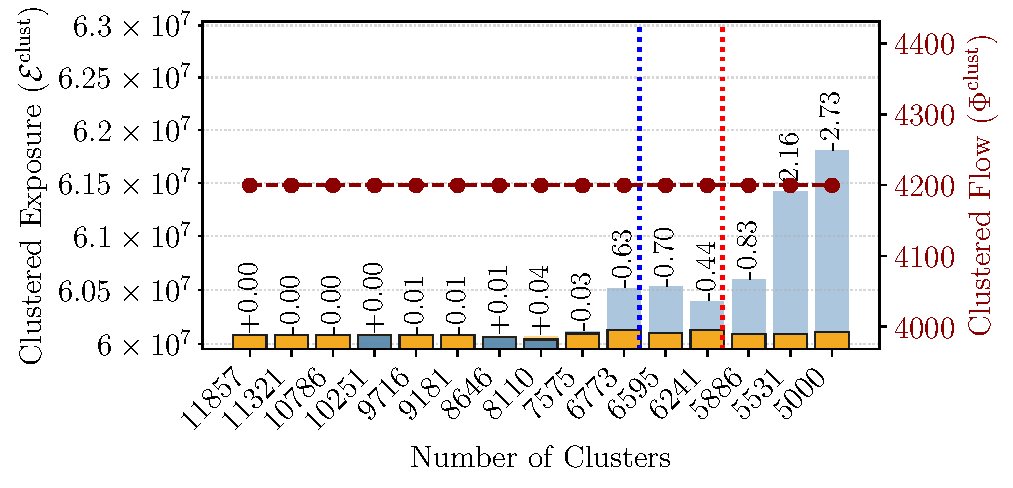
\includegraphics[width=0.48\linewidth]{Images/clustered_expo_flow_overlap_log_Lyon_divergence_CC.pdf}
    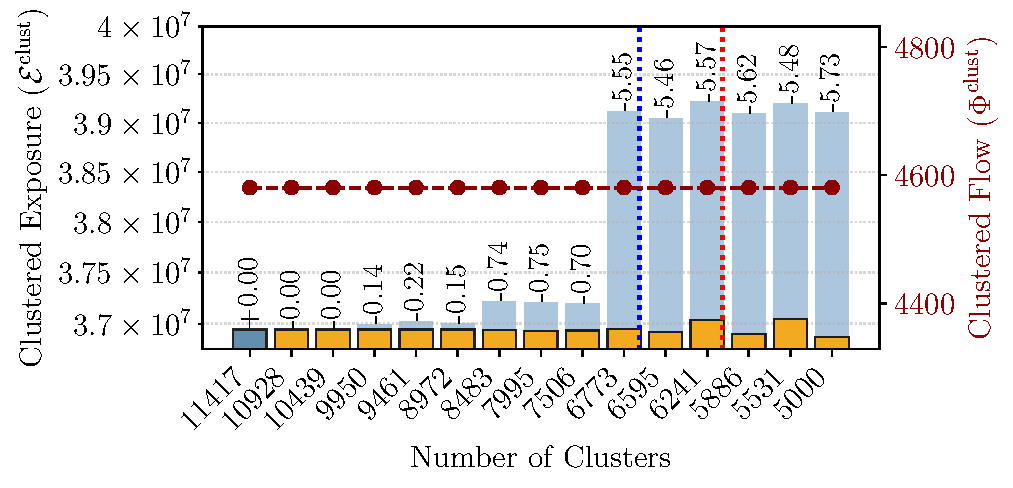
\includegraphics[width=0.48\linewidth]{Images/clustered_expo_flow_overlap_log_Strasbourg_divergence_CC.pdf} %strasbourg
    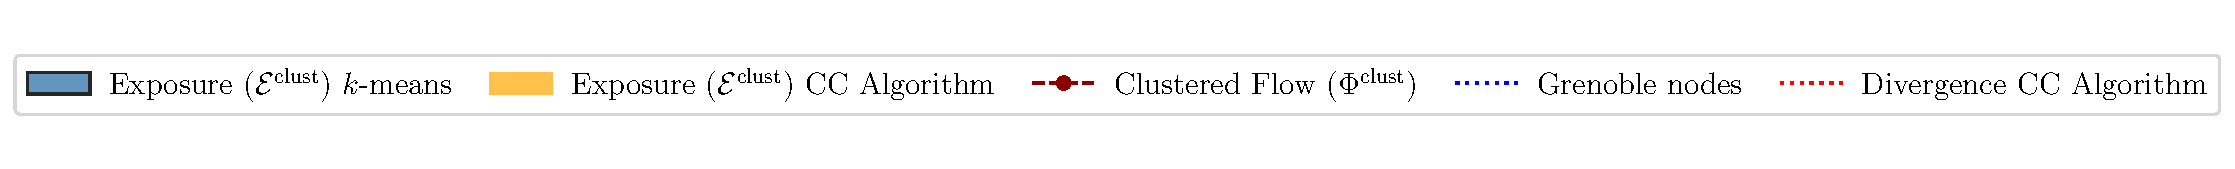
\includegraphics[width=1\linewidth]{Images/legend_expo_flow_CC.pdf}
    \caption{Evolution of cyclist exposure and cyclist flow through the Algorithm A, at the left Lyon and on the right Strasbourg case.}
    \label{fig:exposure_comparison}
\end{figure*}

\subsection{GW-Based Transfer Algorithm (Problem~\ref{prob:gw_transfer_clustered})}

The third algorithm uses the GW correspondence to transfer an optimized strategy
from a source network $\mathcal{H}$ to a target network $\mathcal{G}$. The target
network is first clustered into $\tilde{\mathcal{G}}$ so that
$|\tilde{\mathcal{V}}^{\mathcal{G}}|=|\mathcal{V}^{\mathcal{H}}|$. Then, the GW
transport plan maps source upgrade intensities to clusters of
$\tilde{\mathcal{G}}$. The transferred scores are used to prioritize clustered
objects under the target budget, and the resulting strategy is lifted back to
the original network $\mathcal{G}$.




Algorithms~\ref{alg:ga_original} and~\ref{alg:ga_clustered} approximate the
solutions of the original and clustered bi-level optimization problems,
respectively. Algorithm~\ref{alg:gw_transfer} provides a transfer-based
alternative: it uses the optimized intervention pattern of a structurally similar
source network to guide upgrades on the target network without solving the full
arc-level problem directly.



The algorithms above provide the computational backbone of the proposed
framework. The original GA gives a direct arc-level benchmark, the clustered GA
tests whether optimization can be performed on reduced networks while preserving
the main exposure effects, and the GW-transfer procedure evaluates whether an
optimized strategy from one city can guide interventions in another. We now
apply these three components to real cycling networks in order to assess their
comparability, optimization performance, and transferability.





\section{Case Study}


% \begin{figure*}
%     \centering
%     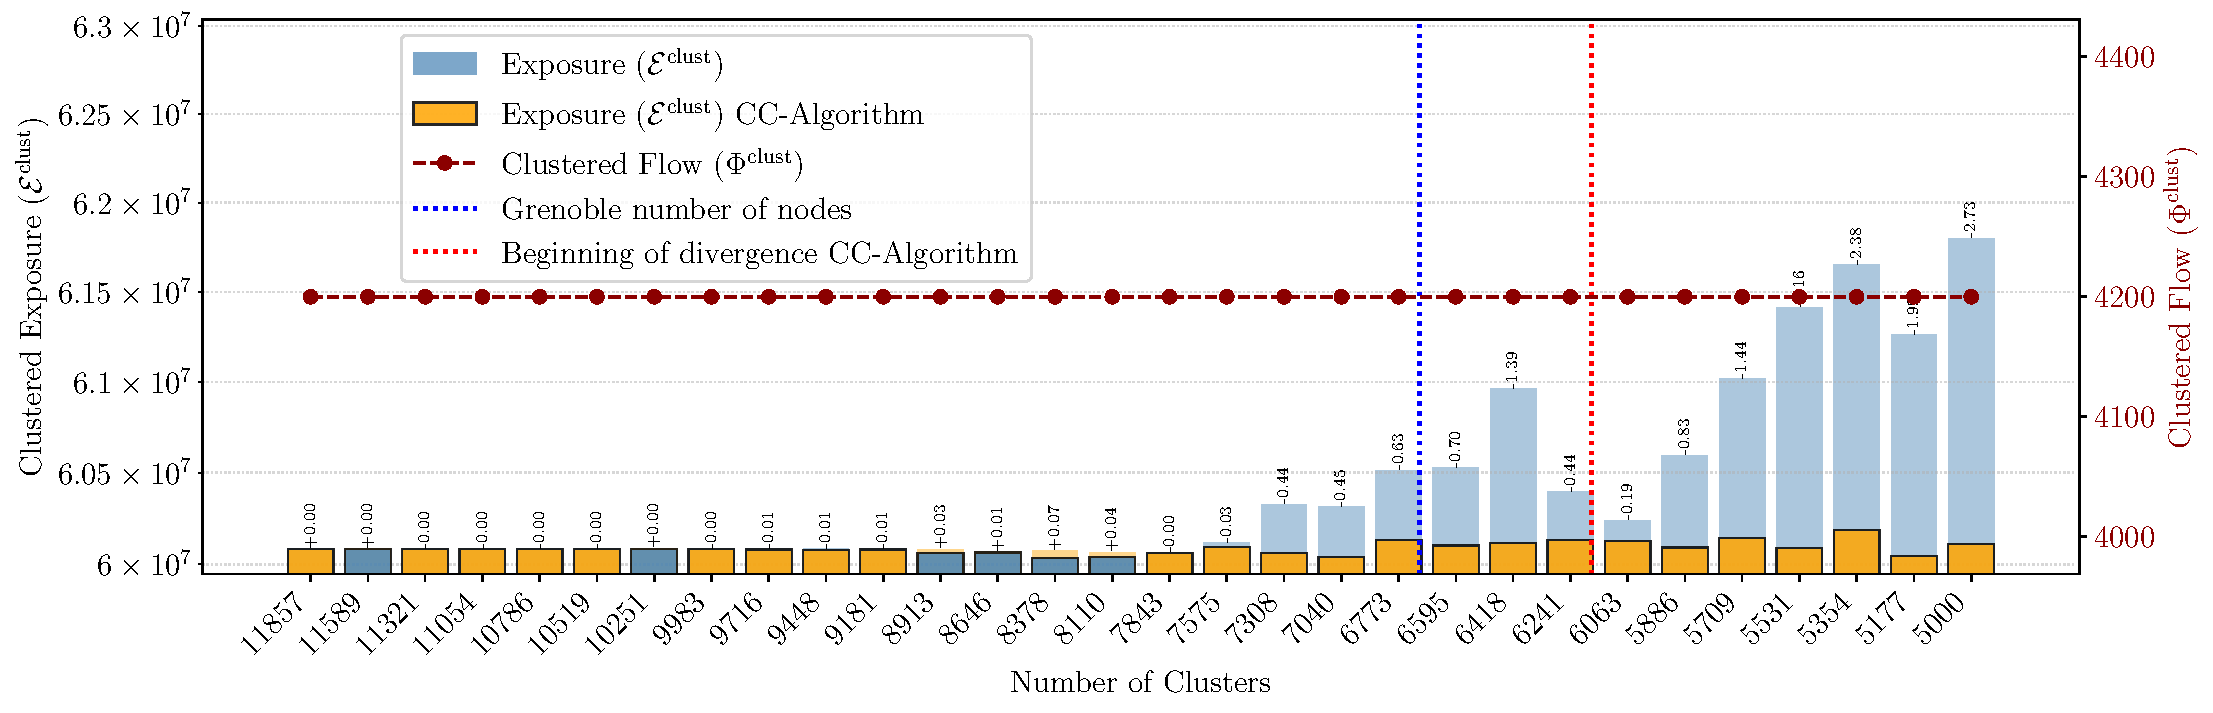
\includegraphics[width=2\columnwidth]{Images/clustered_expo_flow_overlap_log_Lyon_divergence.pdf}\\
%     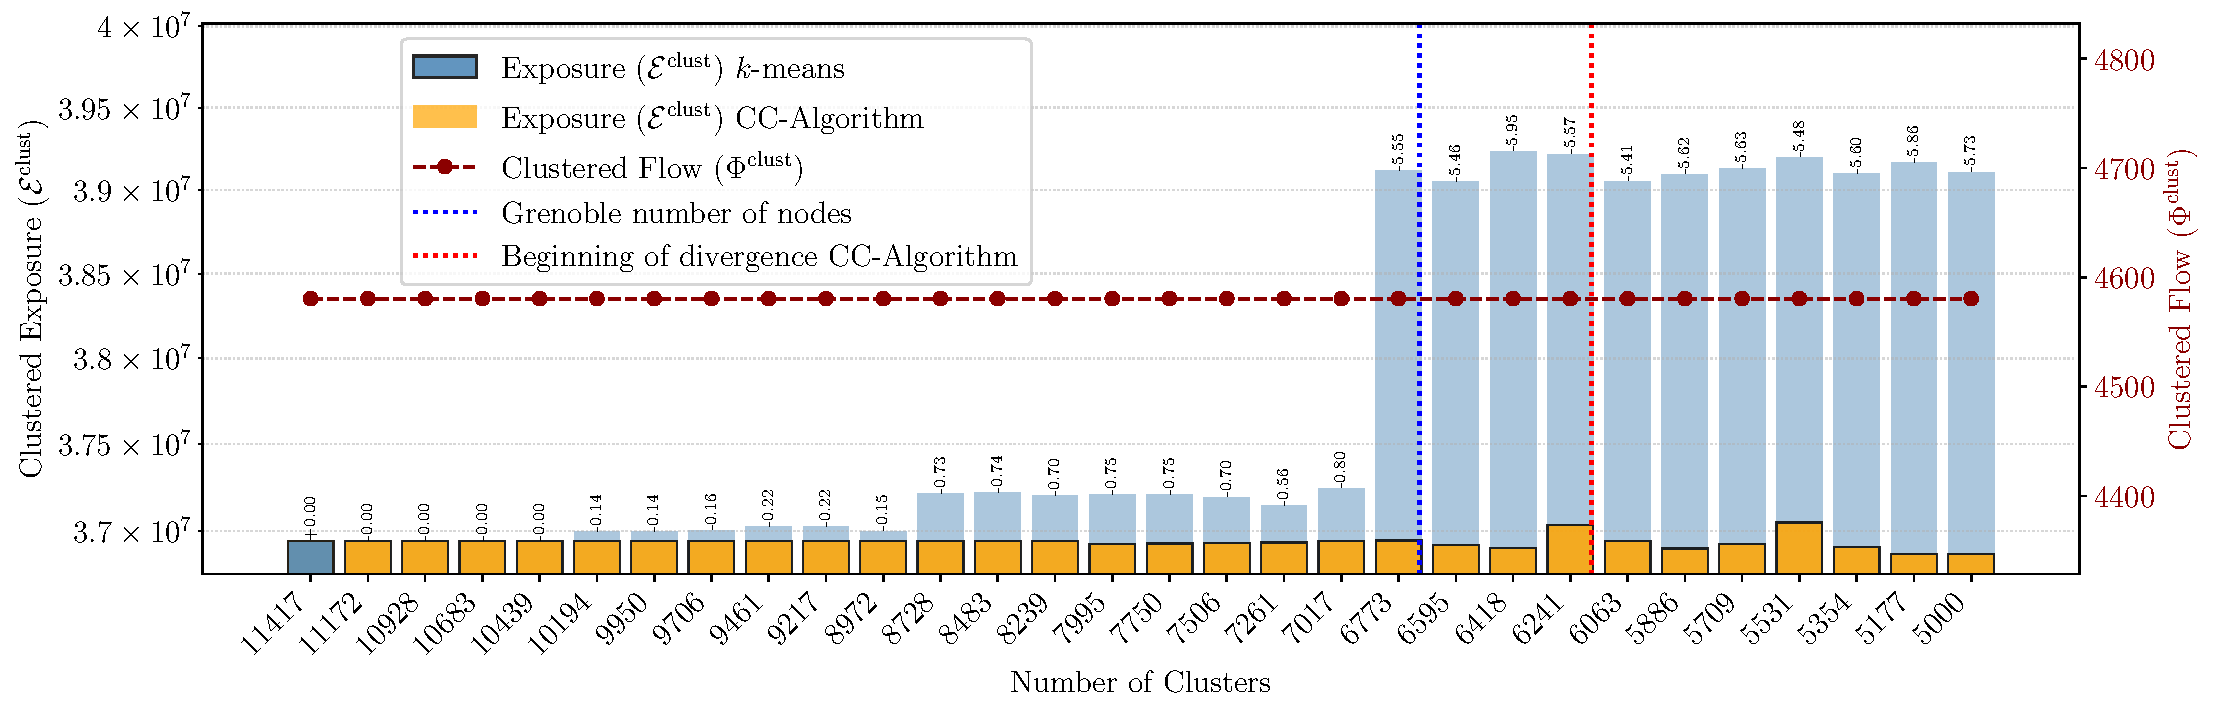
\includegraphics[width=2\columnwidth]{Images/clustered_expo_flow_overlap_log_Strasbourg_divergence.pdf}
%     \caption{Evolution of cyclist exposure and cyclist flow through the Algorithm A, on the top Lyon and on the bottom Strasbourg case.}
%     \label{fig:exposure_comparison}
% \end{figure*}



\begin{figure*}[t]
\centering
\captionsetup[subfigure]{font={footnotesize}, labelfont={footnotesize, bf}, textfont={footnotesize, rm}}
\subfloat[Original]{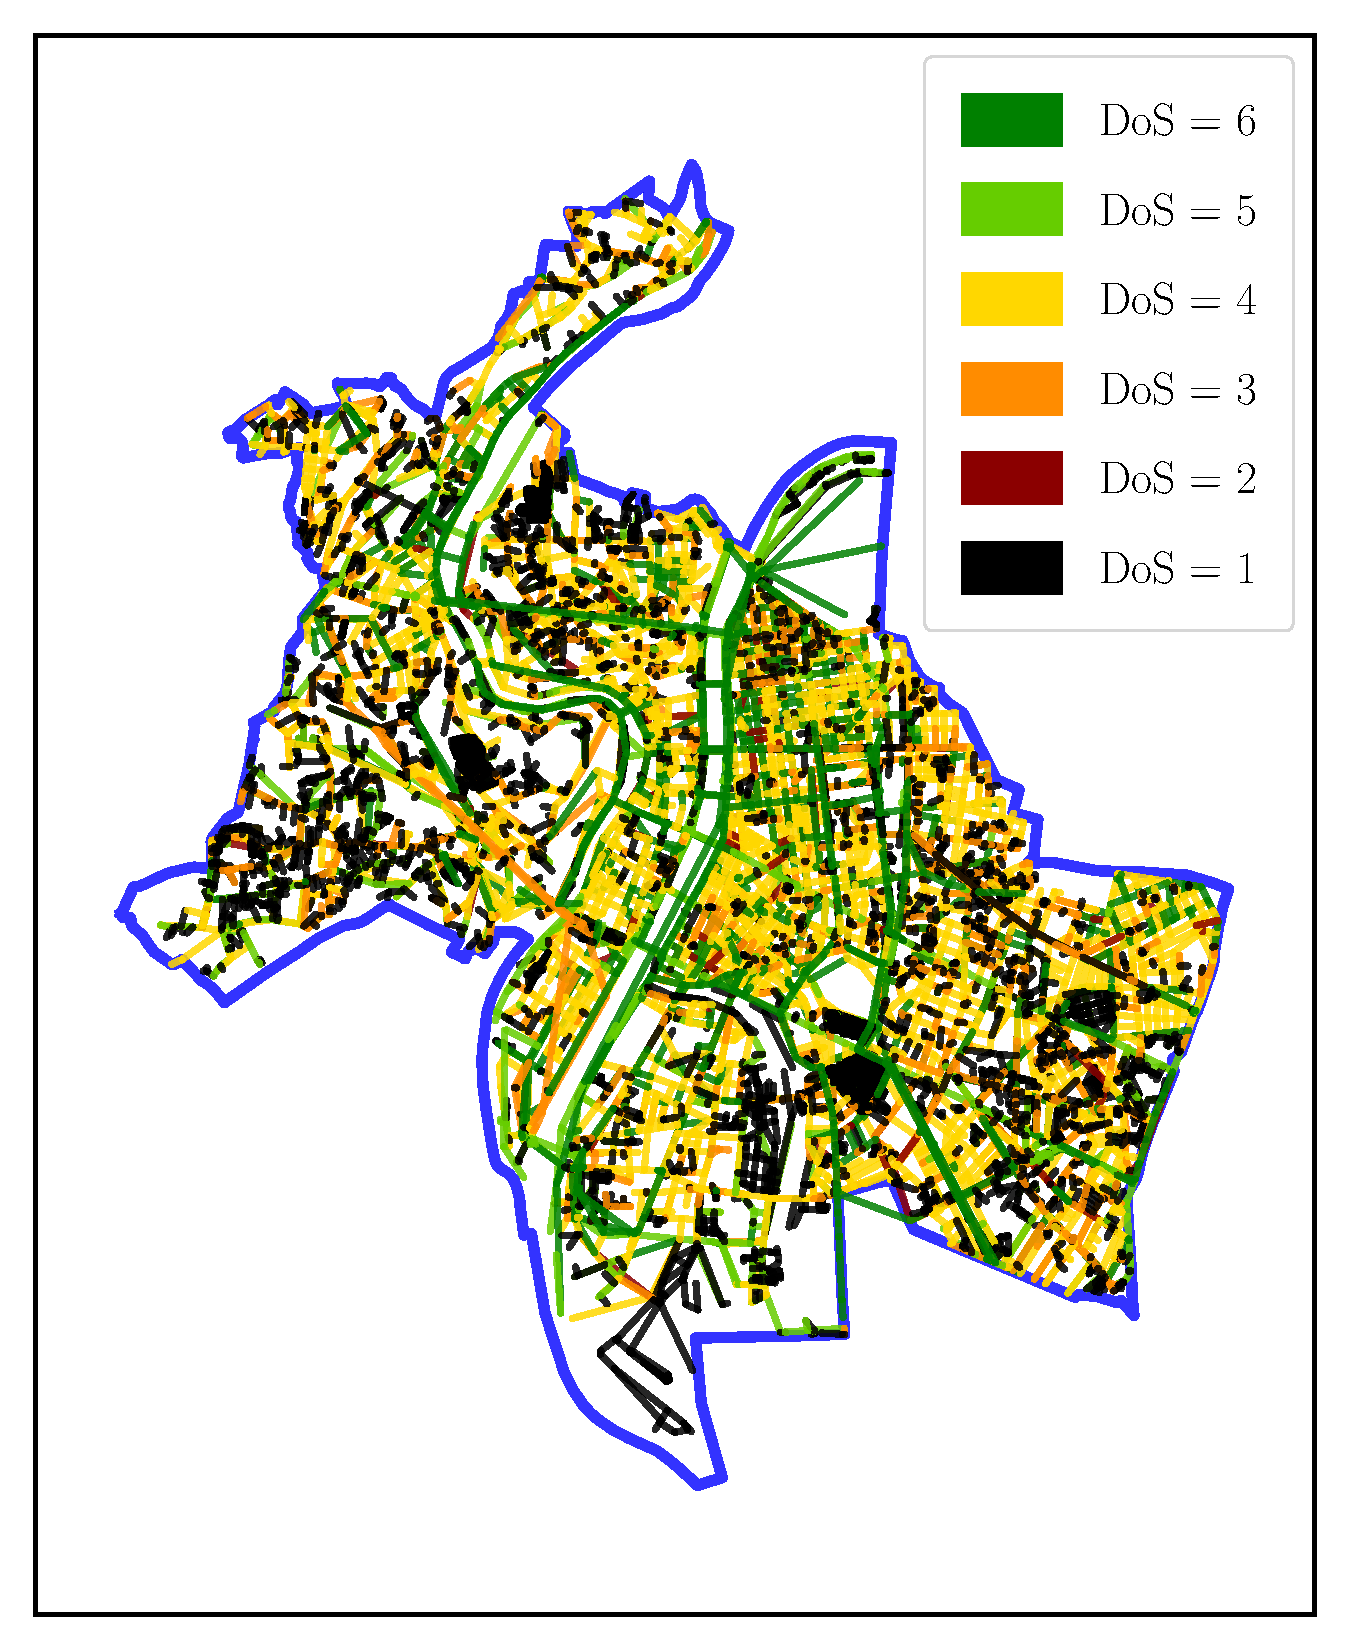
\includegraphics[width=0.49\columnwidth]{Images/Lyon_DoS.pdf}}
\subfloat[$K$-mean]{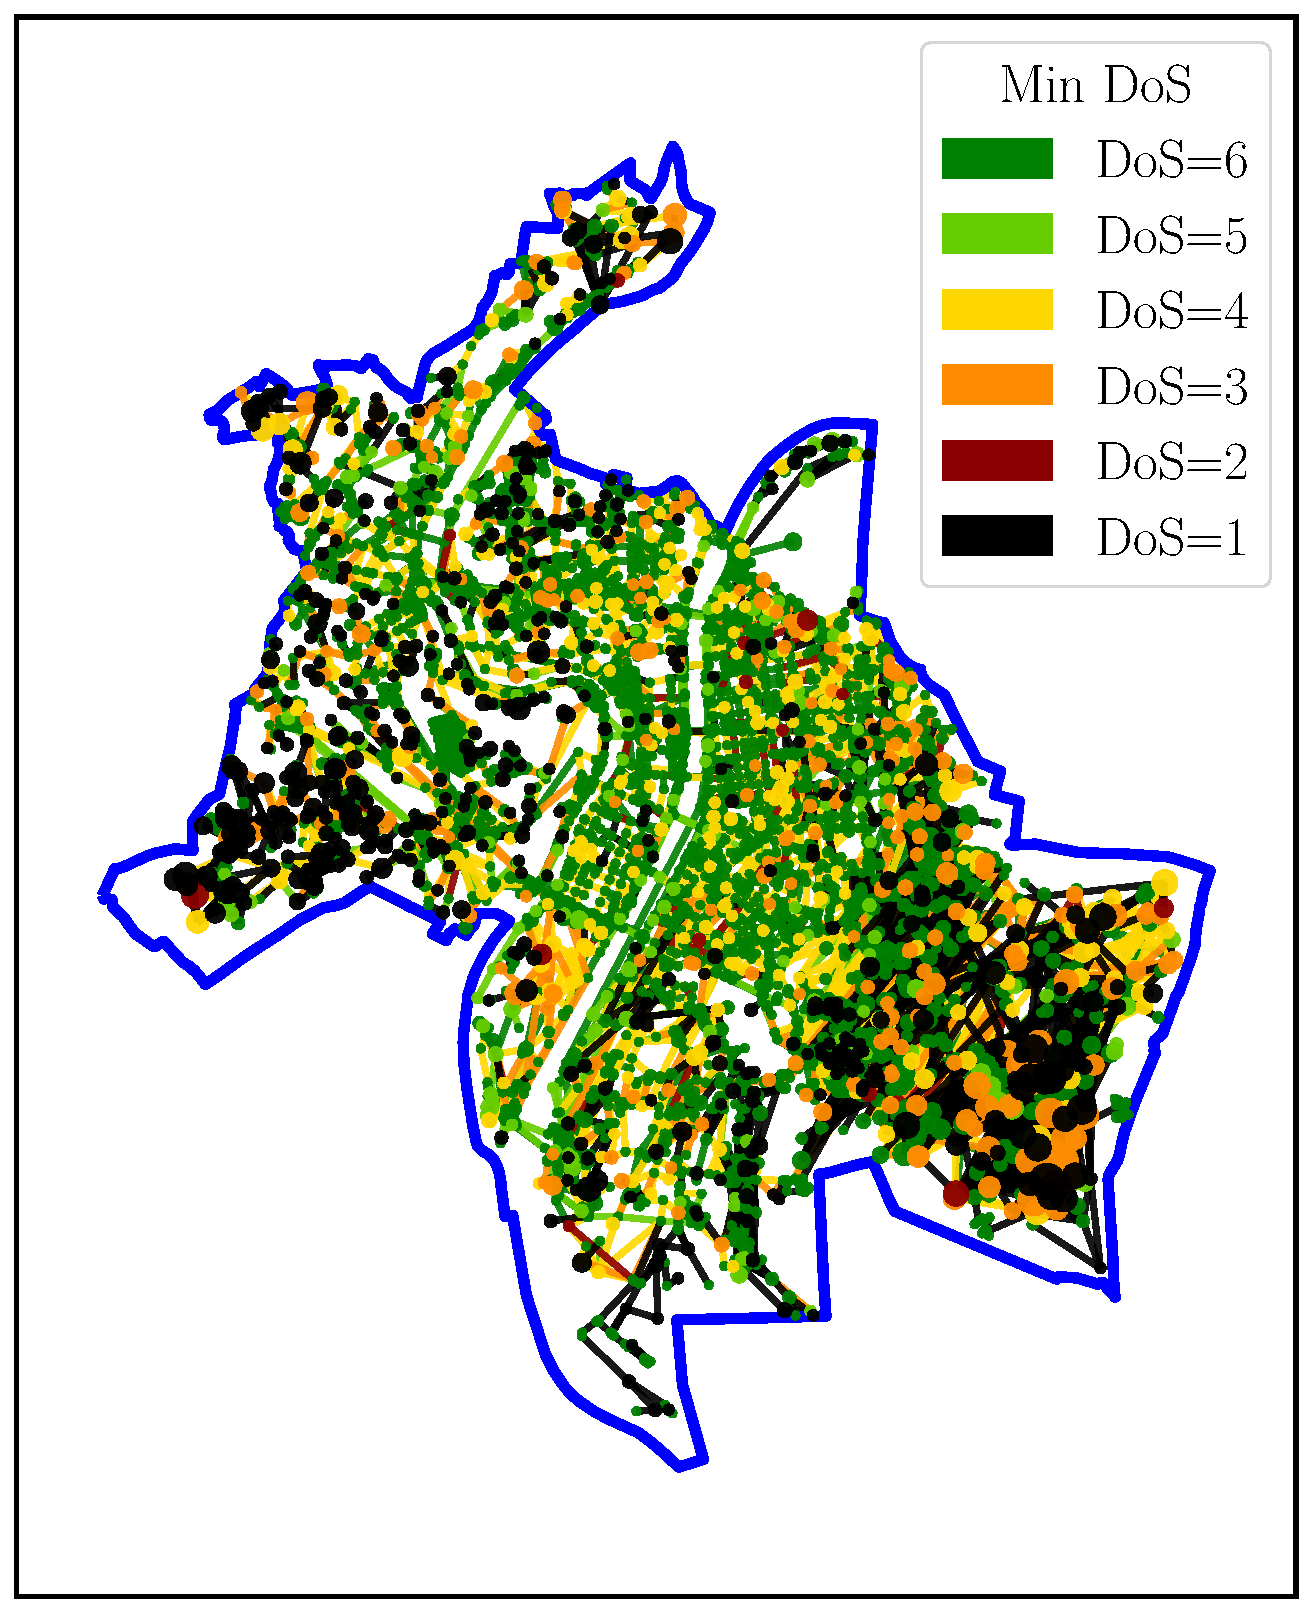
\includegraphics[width=0.48\columnwidth]{Images/H_clust_by_key_Lyon_algorithm.pdf}}
\subfloat[CC-Algorithm]{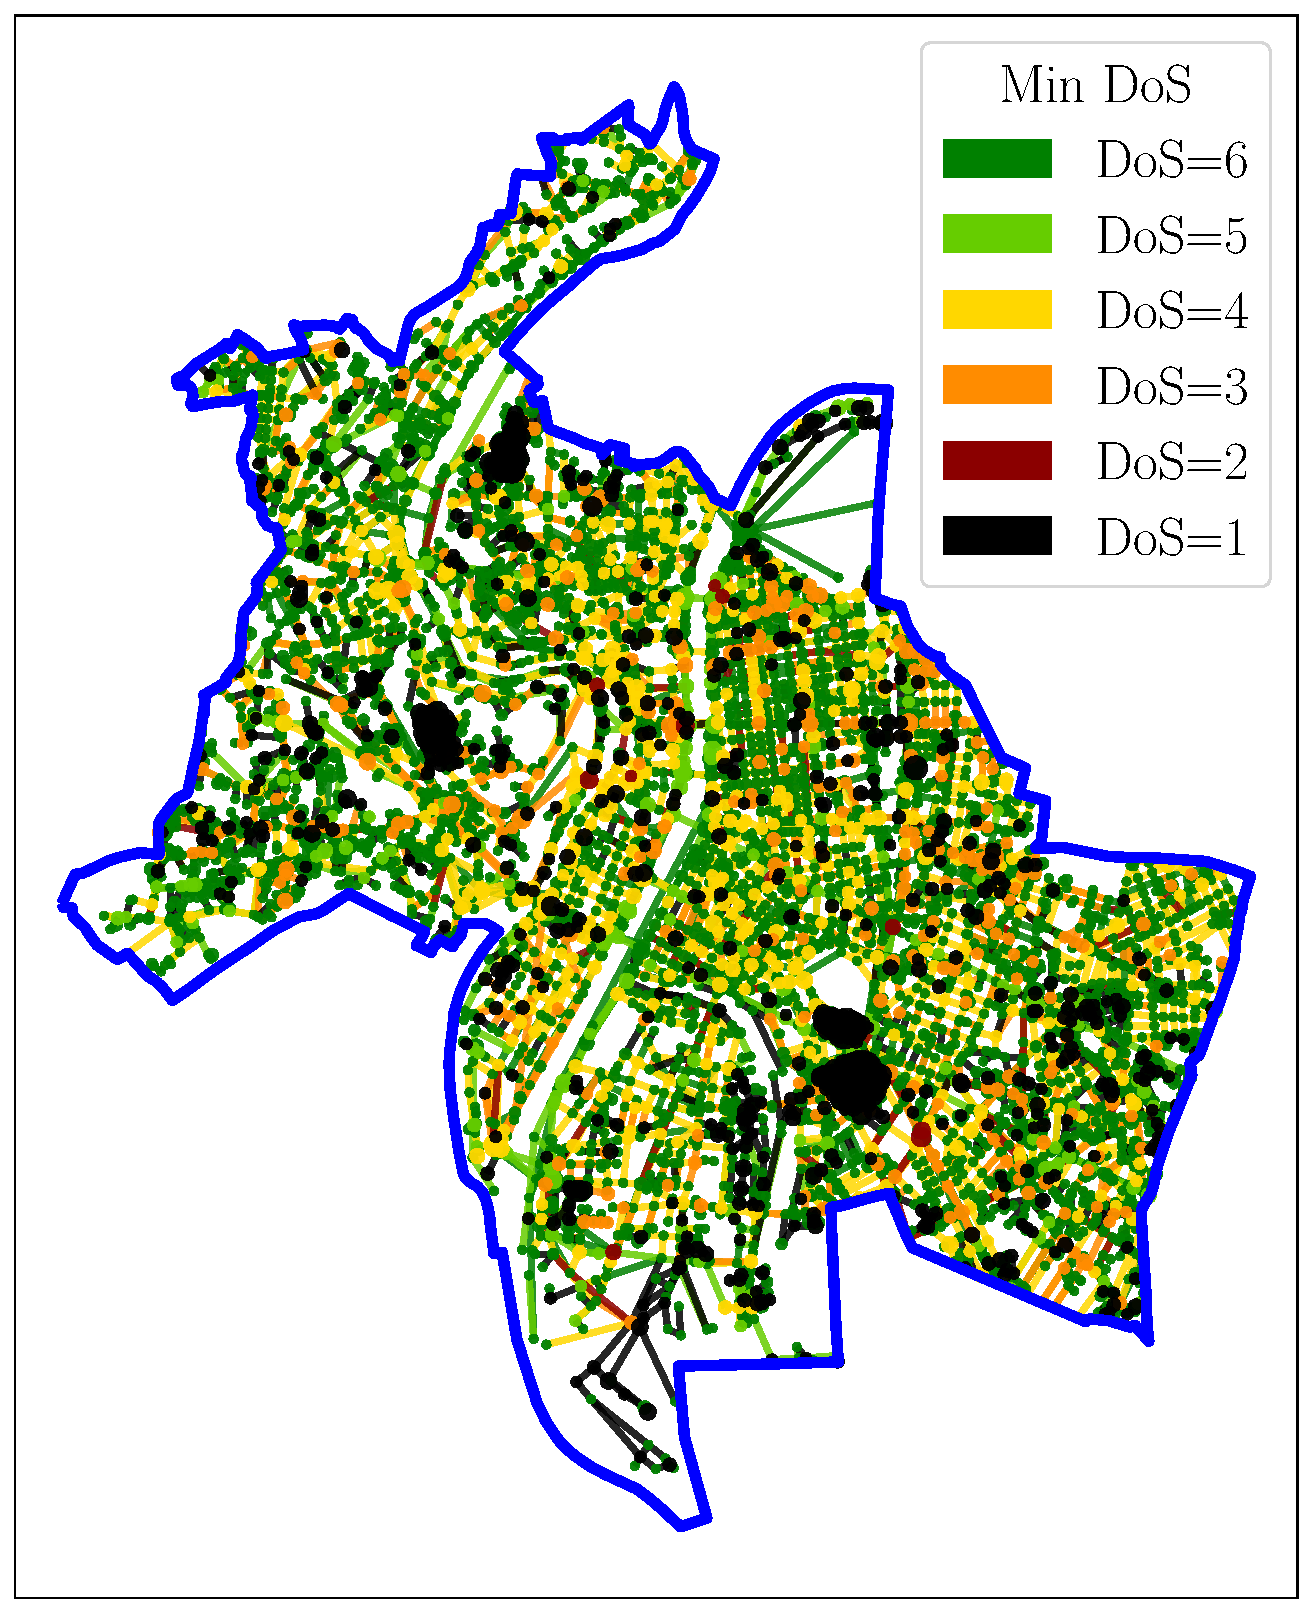
\includegraphics[width=0.48\columnwidth]{Images/clustered_dos_Lyon_1.pdf}}\\
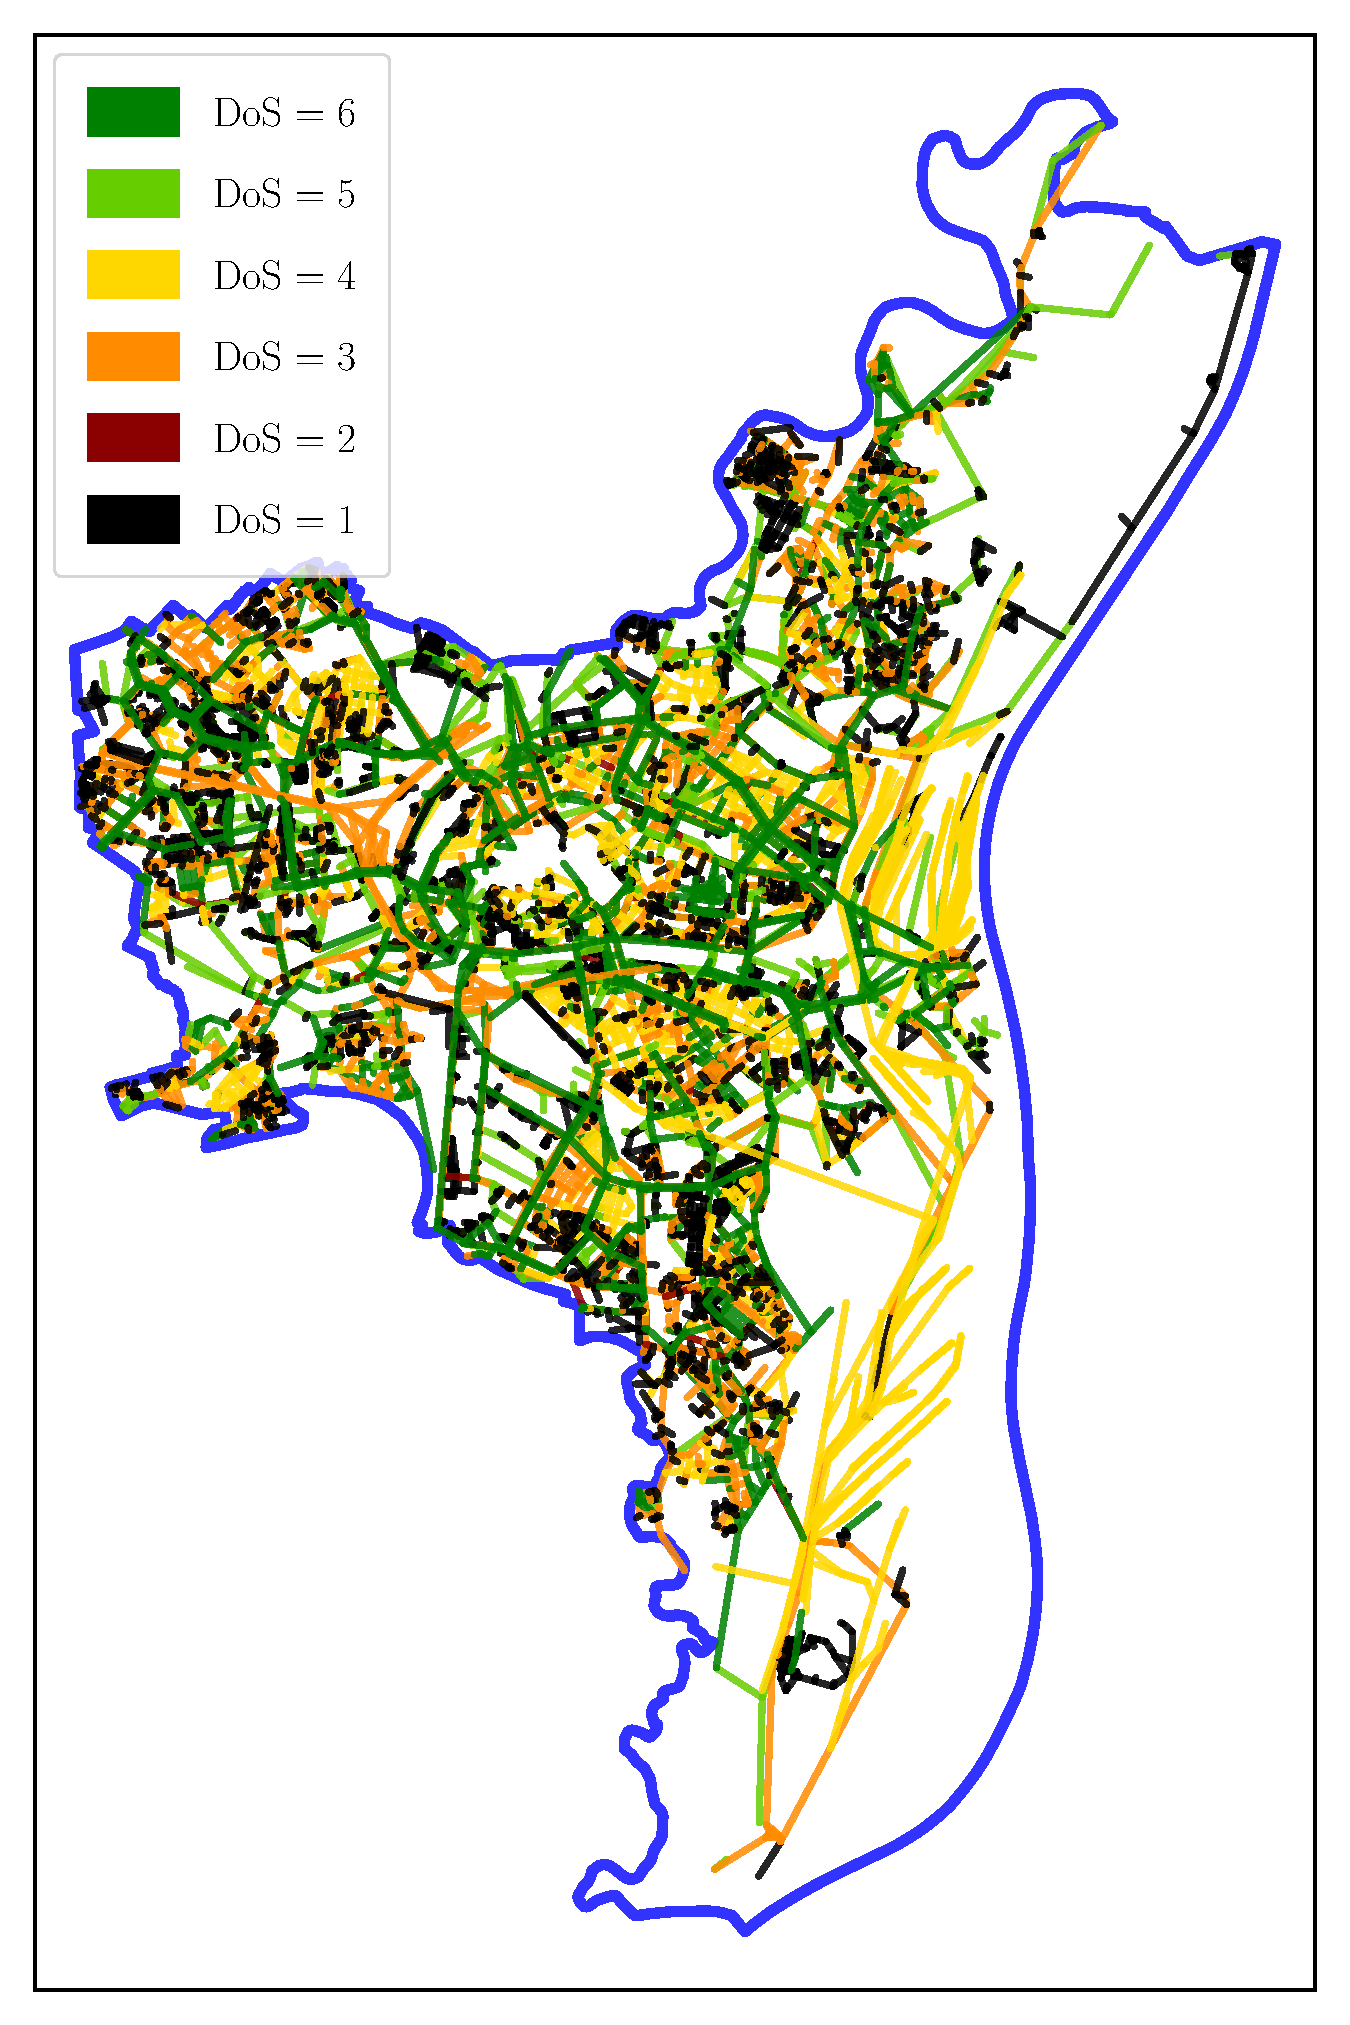
\includegraphics[width=0.485\columnwidth]{Images/Stasbourg_DoS_2.pdf}
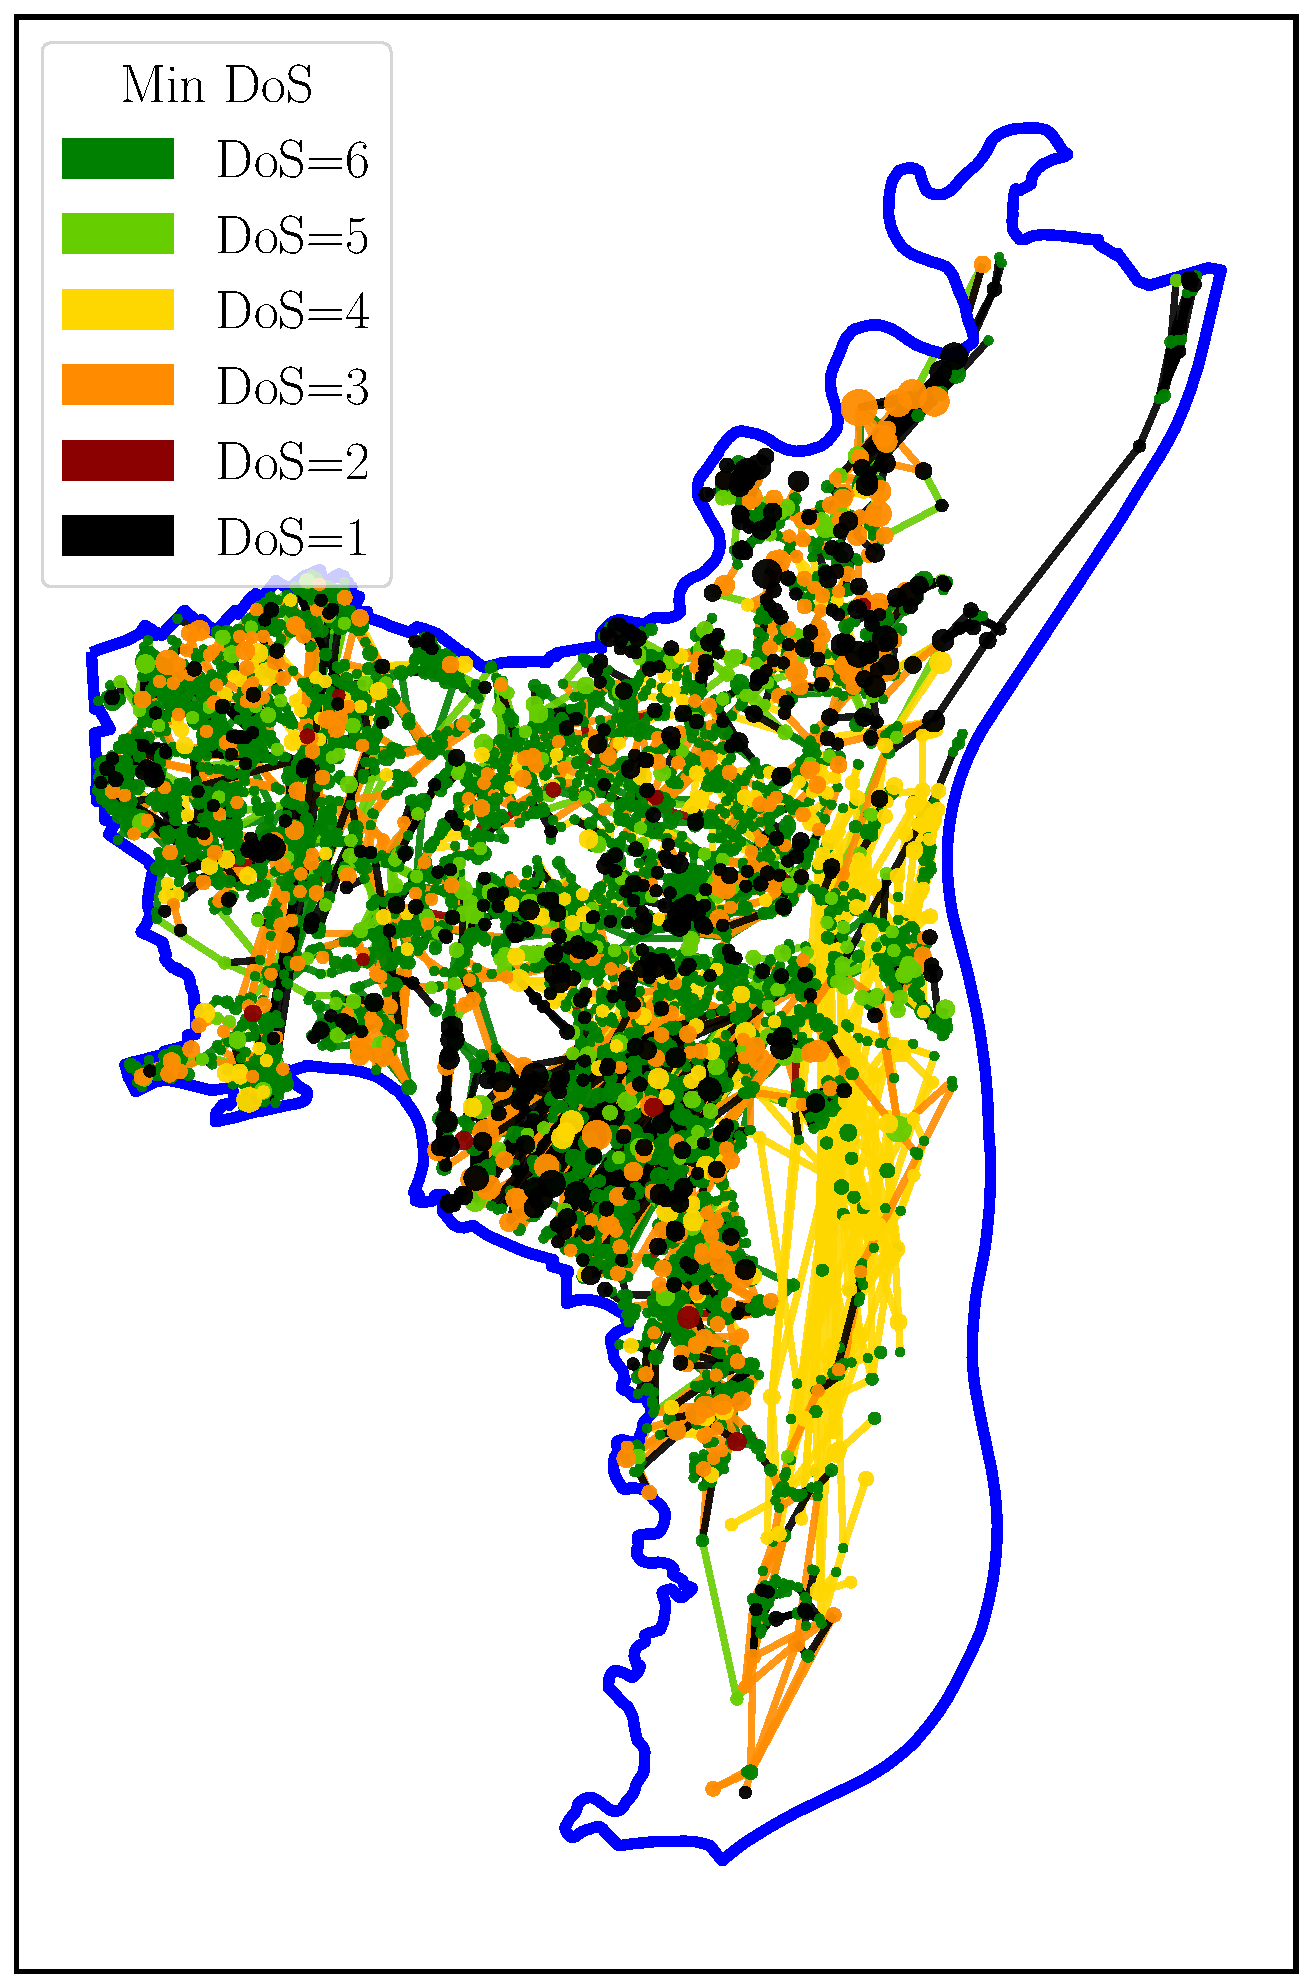
\includegraphics[width=0.48\columnwidth]{Images/H_clust_by_key_strasbourg_algorithm.pdf}
% 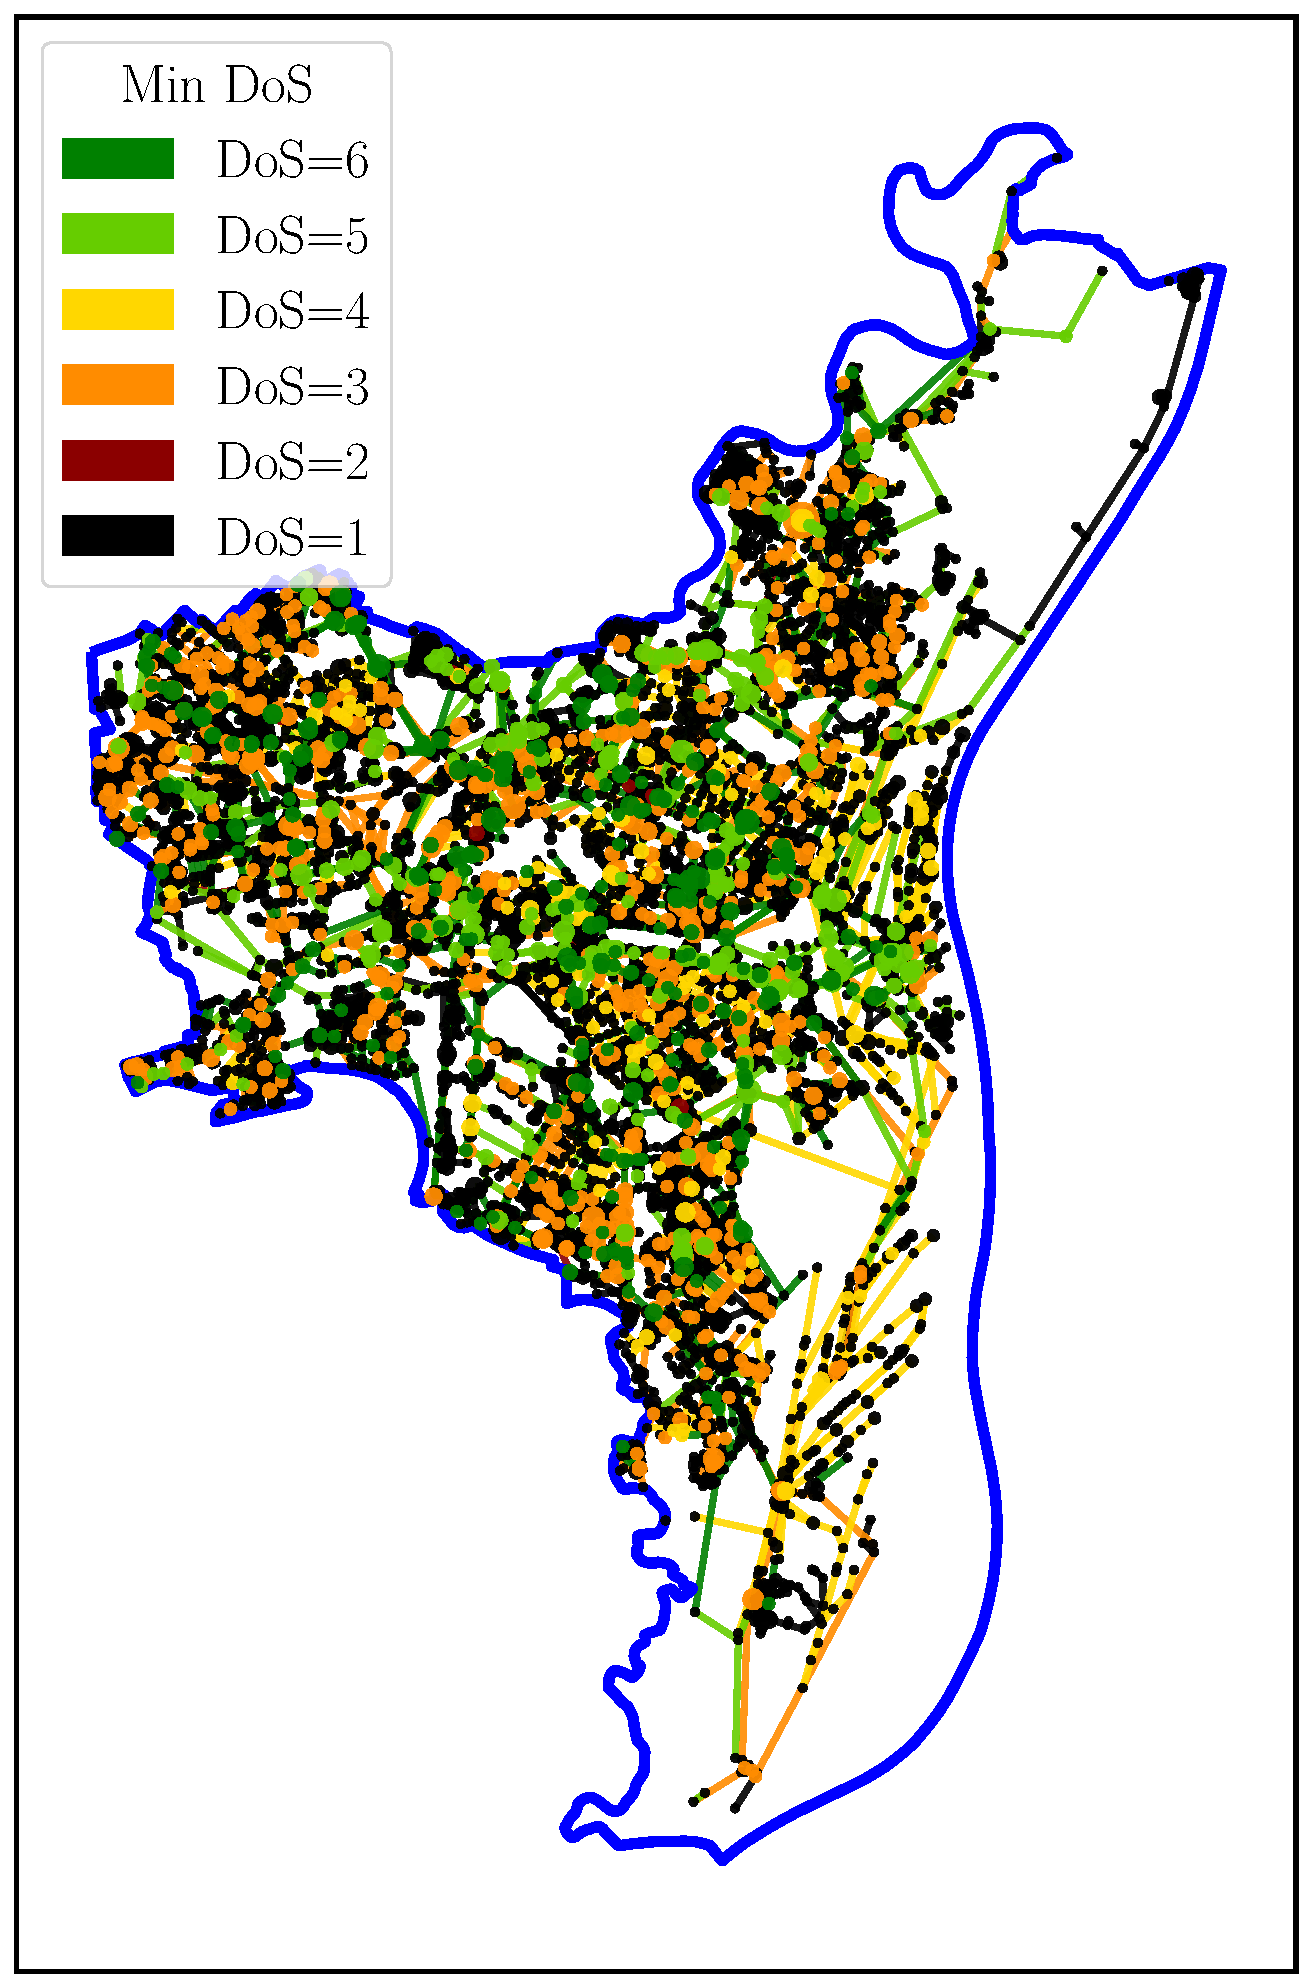
\includegraphics[width=0.48\columnwidth]{Images/H_clust_by_key_strasbourg.pdf}
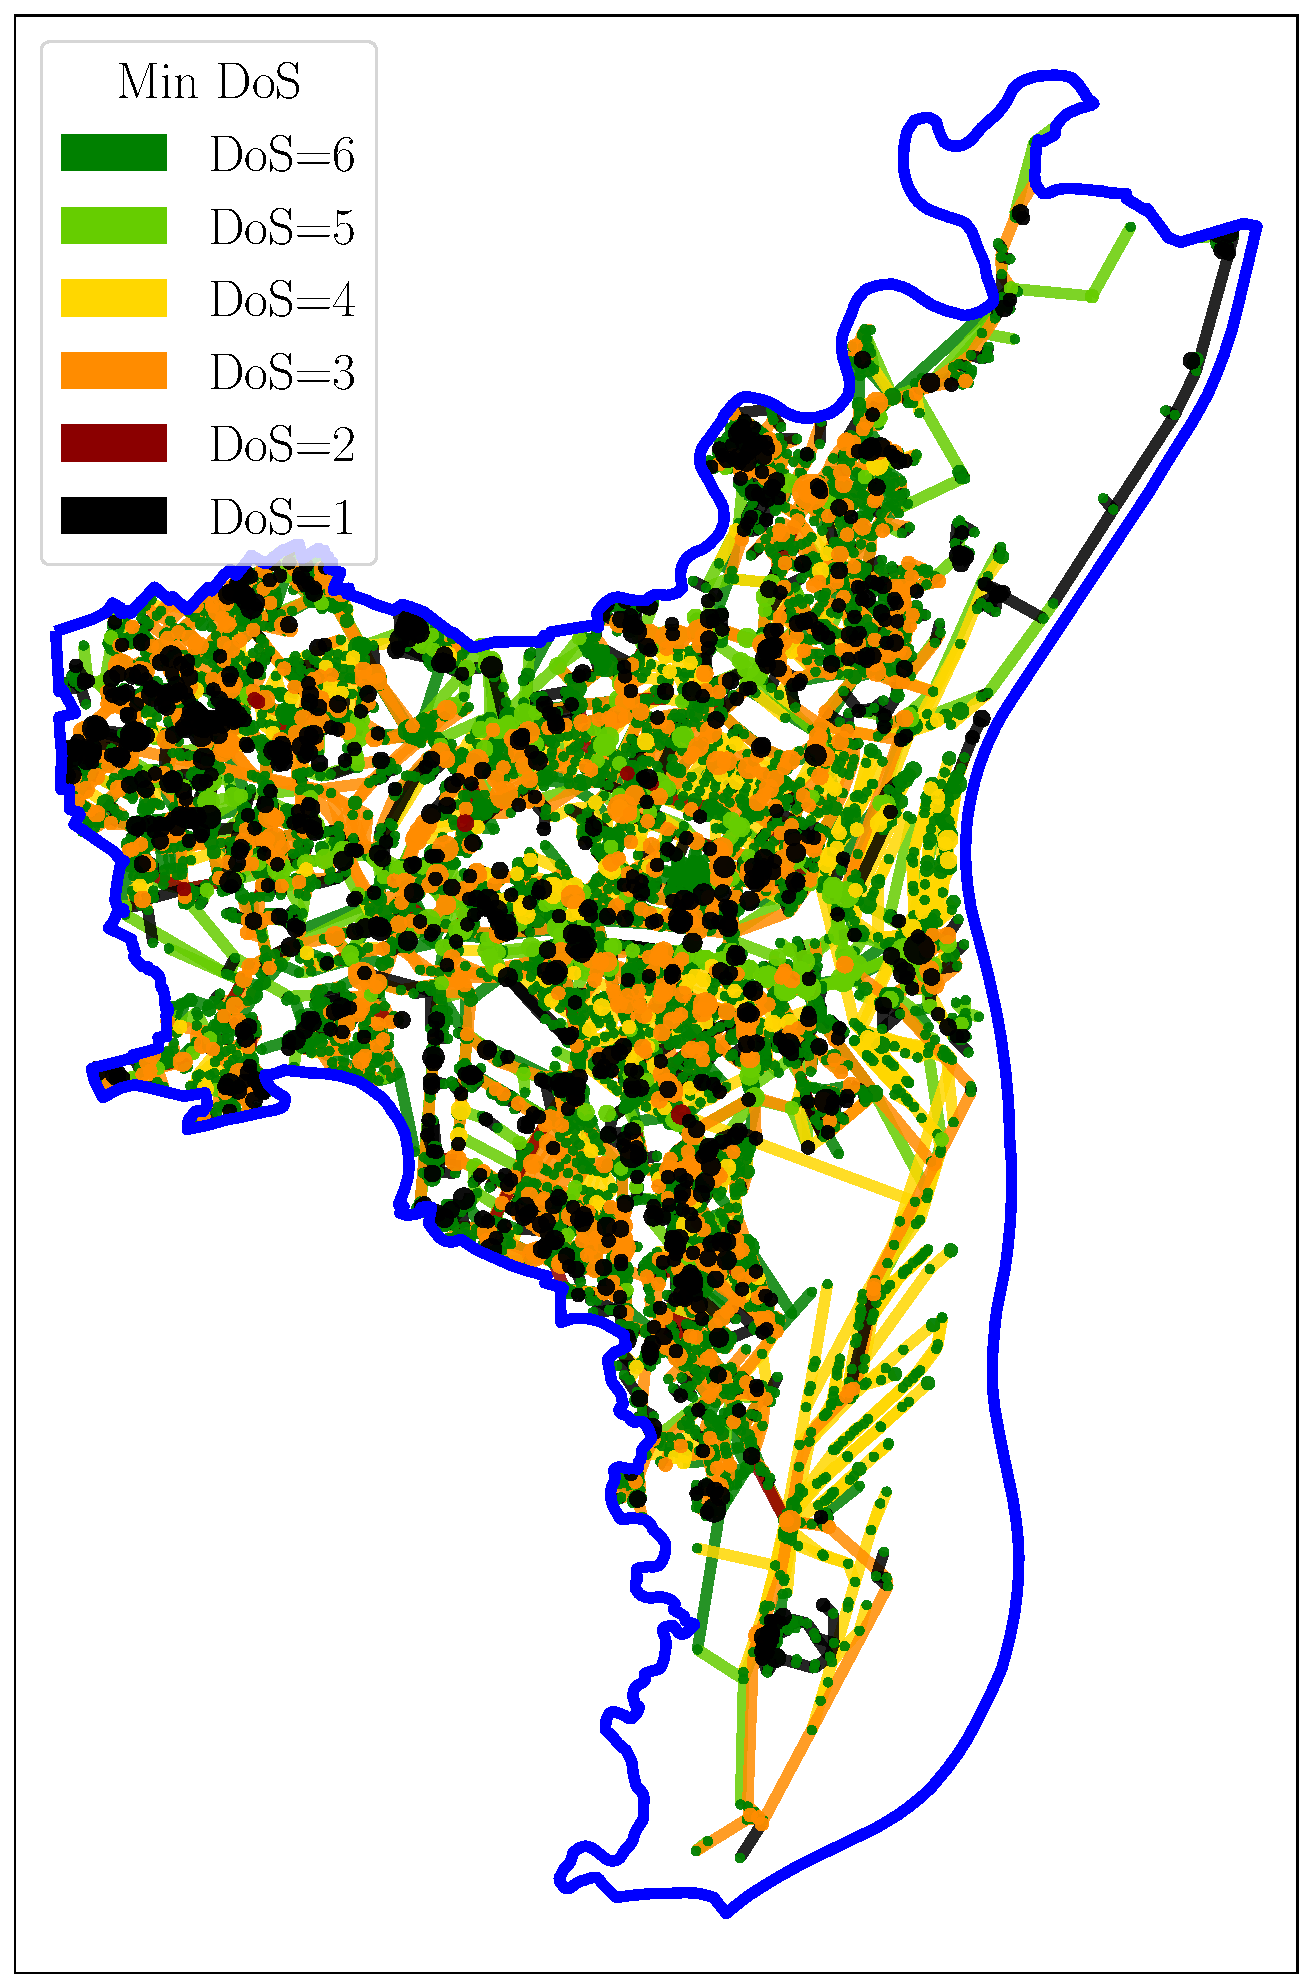
\includegraphics[width=0.48\columnwidth]{Images/clustered_dos_Strasbourg_1.pdf}
\caption{\footnotesize Clustering process with CC-Algorithm, on the first column we have the original networks, then the cluster one with $K$-mean and finally with CC-Algorithm.}
\label{fig:cluster_comparison_topology}
\end{figure*}

\begin{figure}[t]
    \centering
    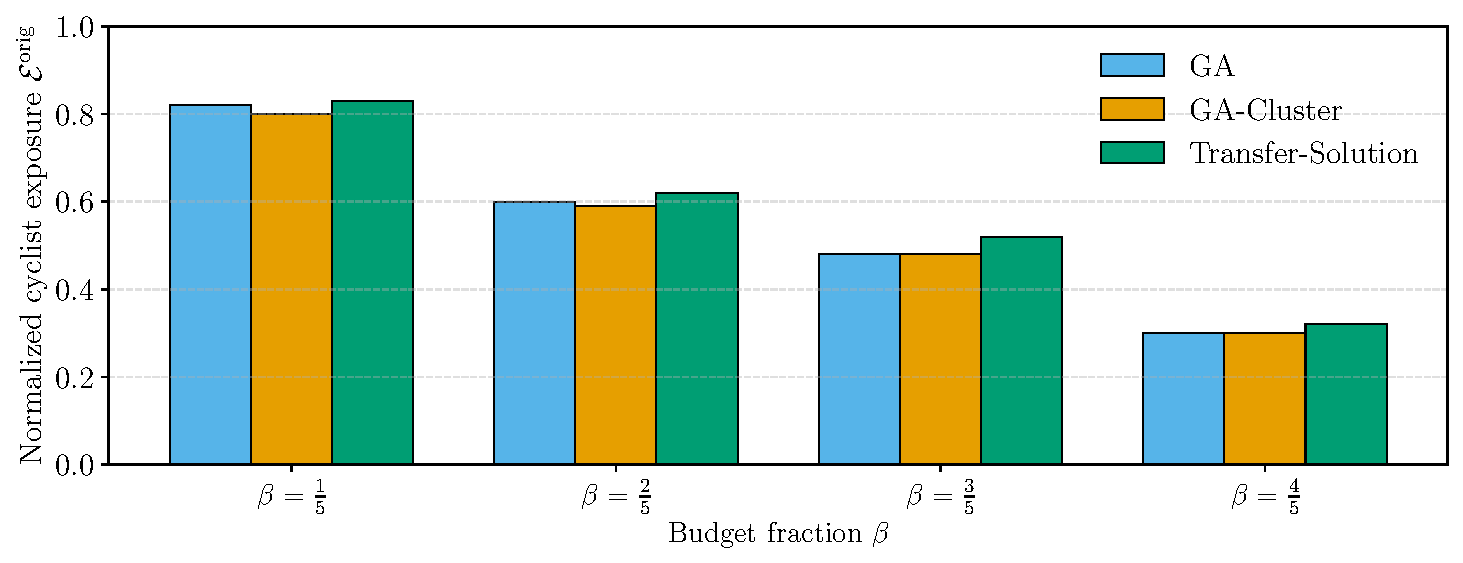
\includegraphics[width=1\columnwidth]{Images/normalized_cyclist_exposure_budget.pdf}\\
    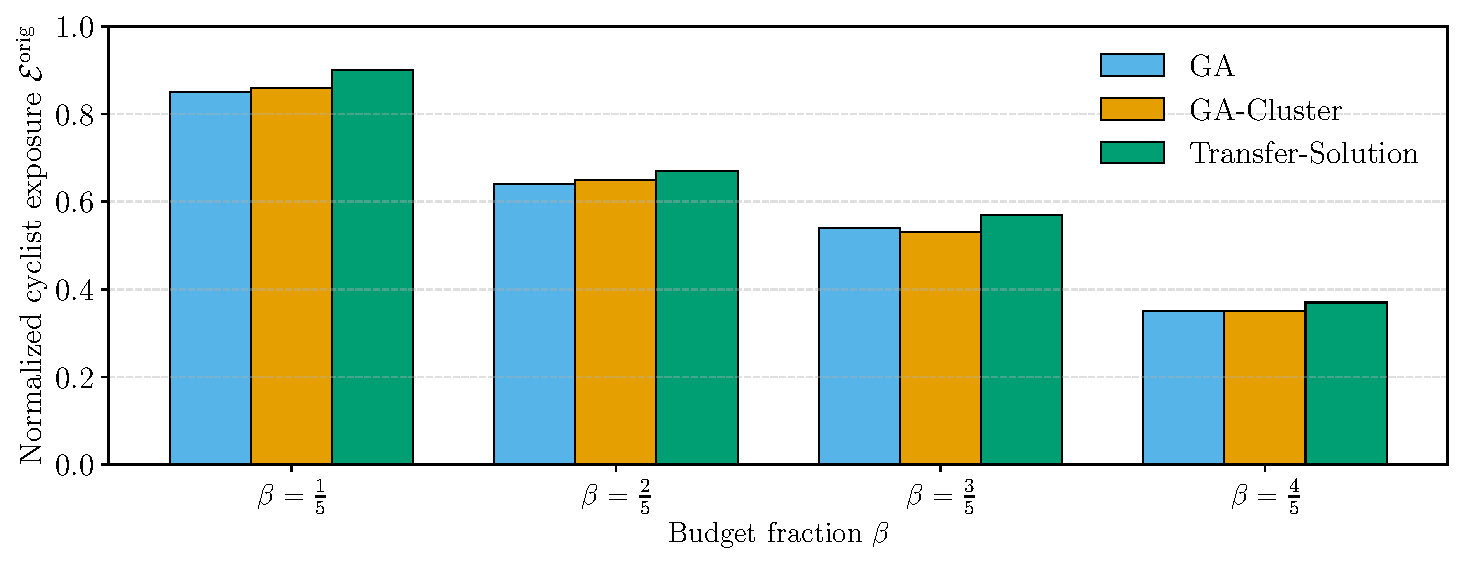
\includegraphics[width=1\columnwidth]{Images/normalized_cyclist_exposure_budget_Lyon.pdf}\\

    \caption{Normalized cyclist traffic exposure under different optimization strategies: top, Strasbourg; bottom, Lyon.}
    \label{fig:exposure_barplots}
\end{figure}


\begin{figure}[ht]
    \centering
    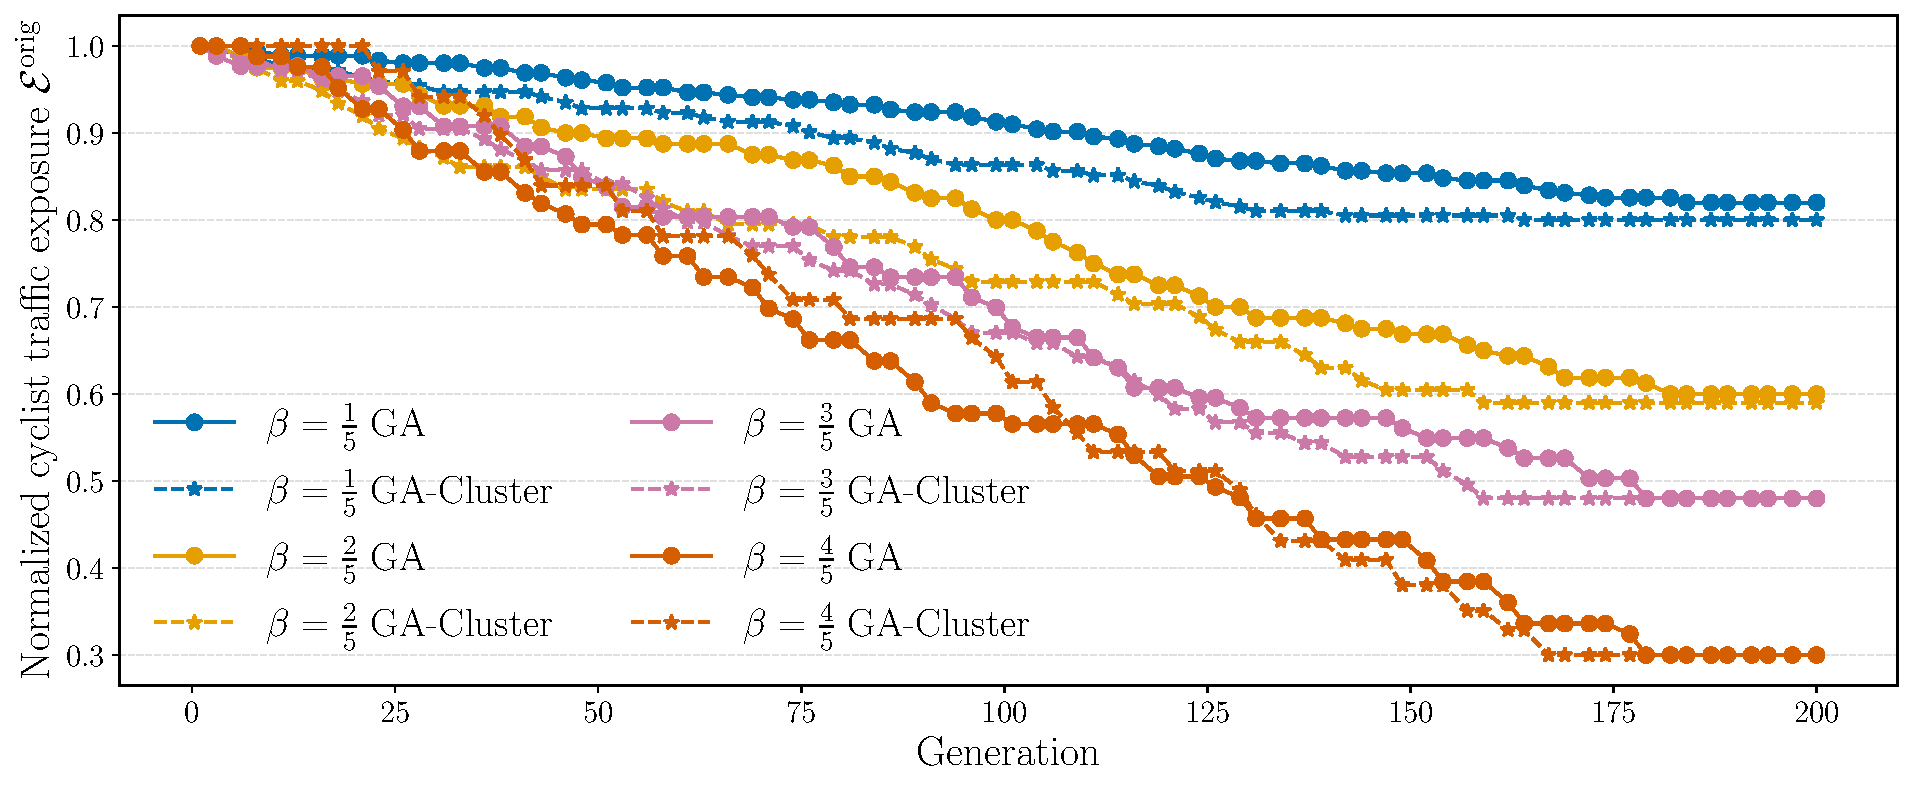
\includegraphics[width=1\columnwidth]{Images/exposure_evolution_all_budgets.pdf}\\
    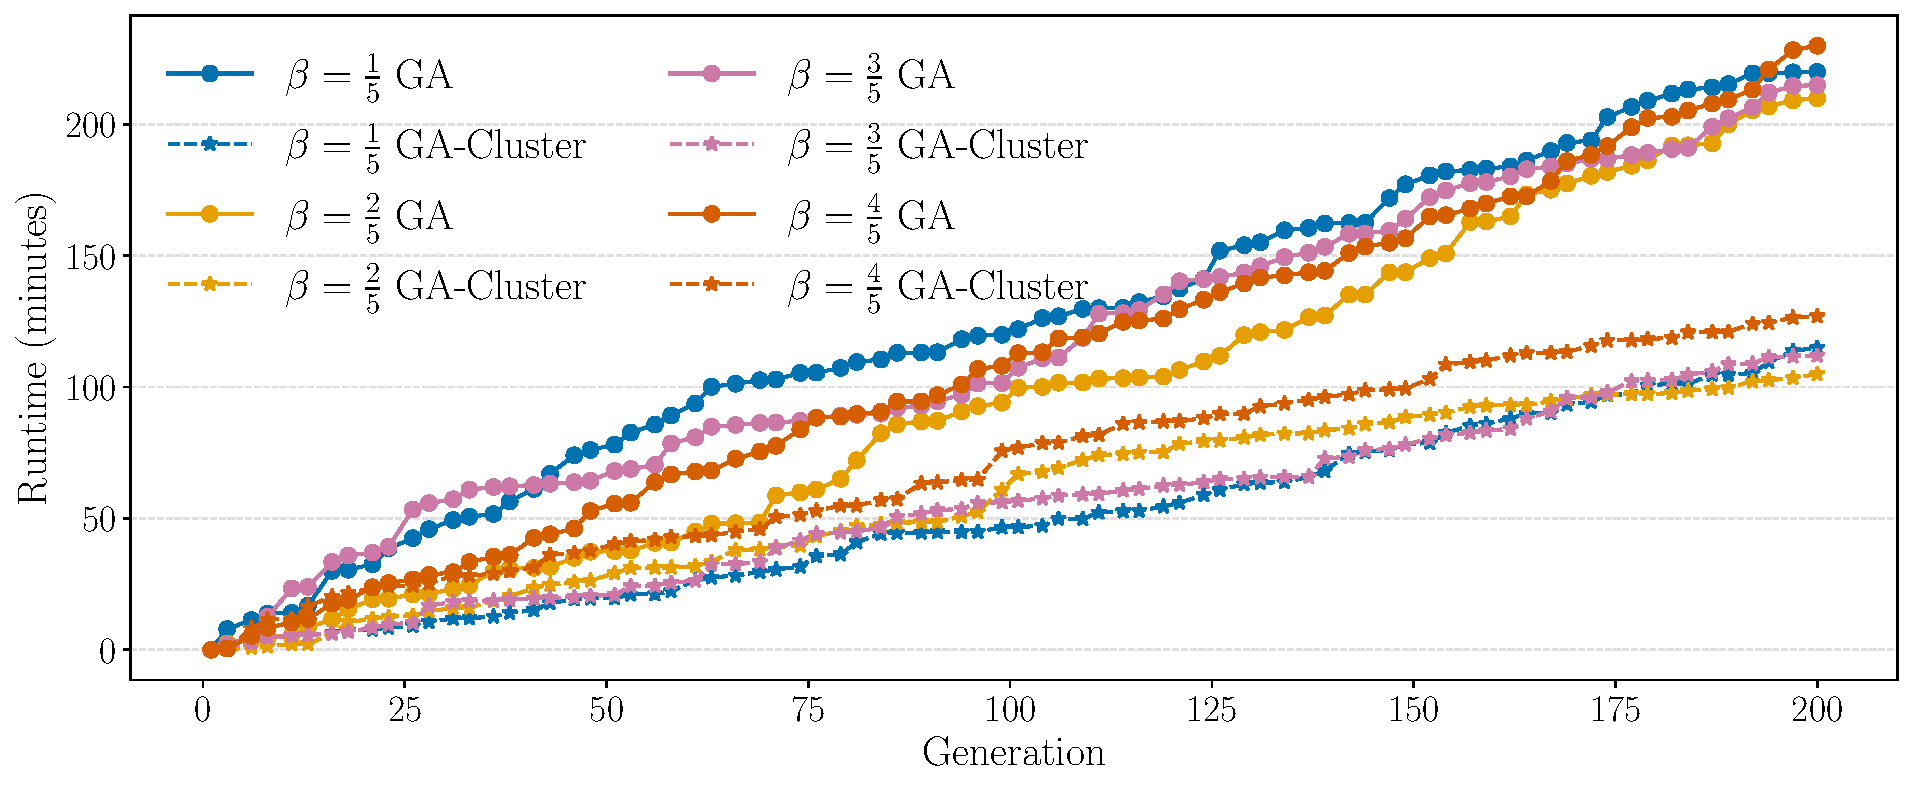
\includegraphics[width=1\columnwidth]{Images/runtime_evolution_all_budgets.pdf}\\

    \caption{Evolution of normalized cyclist traffic exposure and runtime over generations}
    \label{fig:algorithms_convergence}
\end{figure}


\begin{figure*}[t]
\centering
\captionsetup[subfigure]{font={footnotesize}, labelfont={footnotesize, bf}, textfont={footnotesize, rm}}
\subfloat[Original Strasbourg]{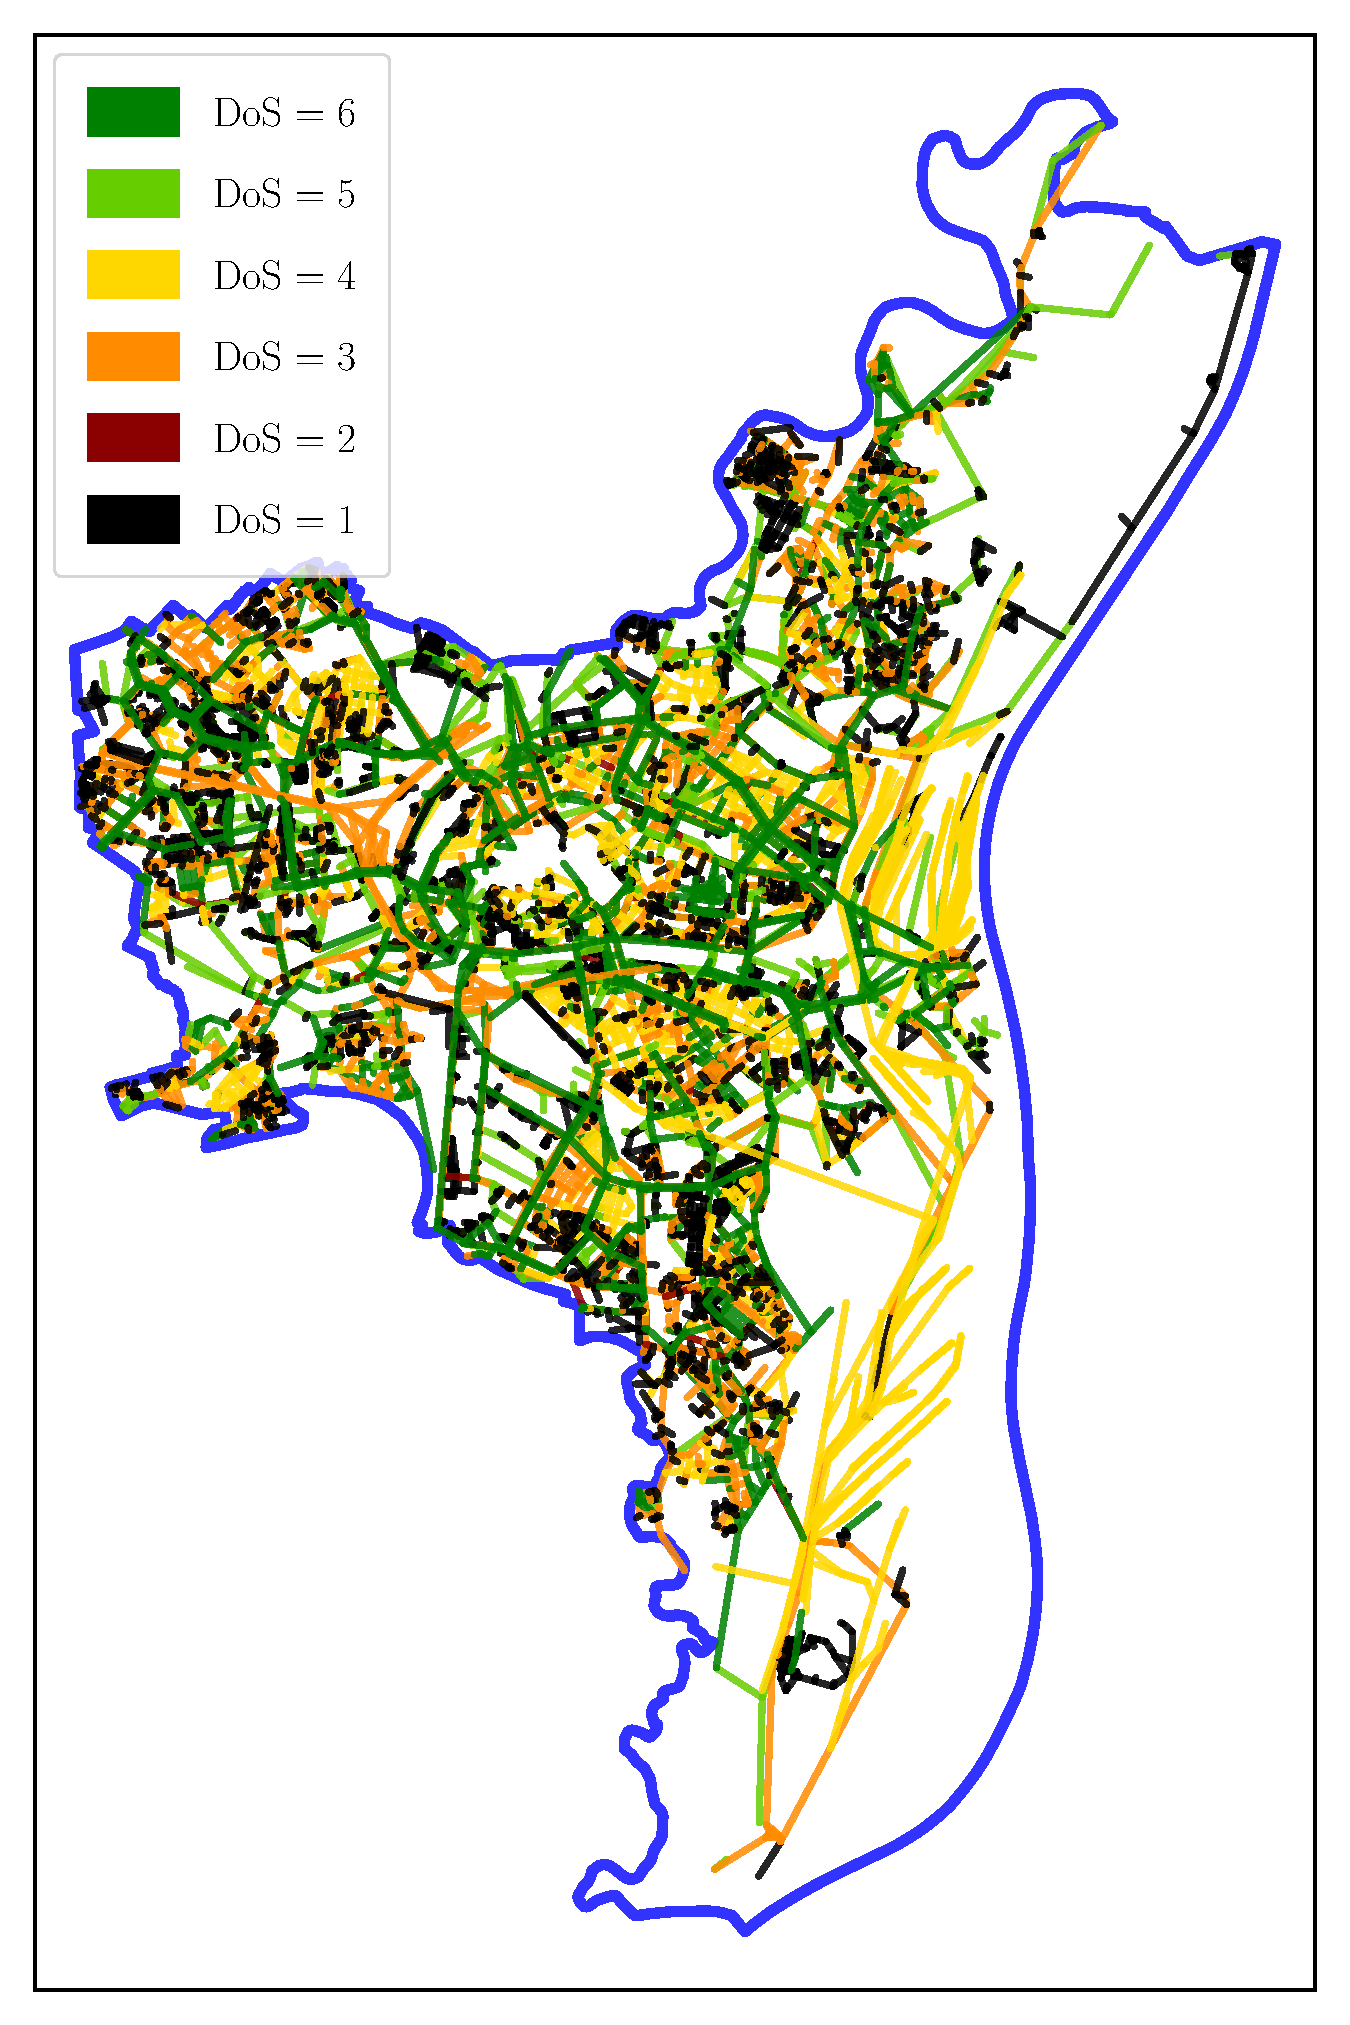
\includegraphics[width=0.48\columnwidth]{Images/Stasbourg_DoS_2.pdf}}
\subfloat[GA on original network]{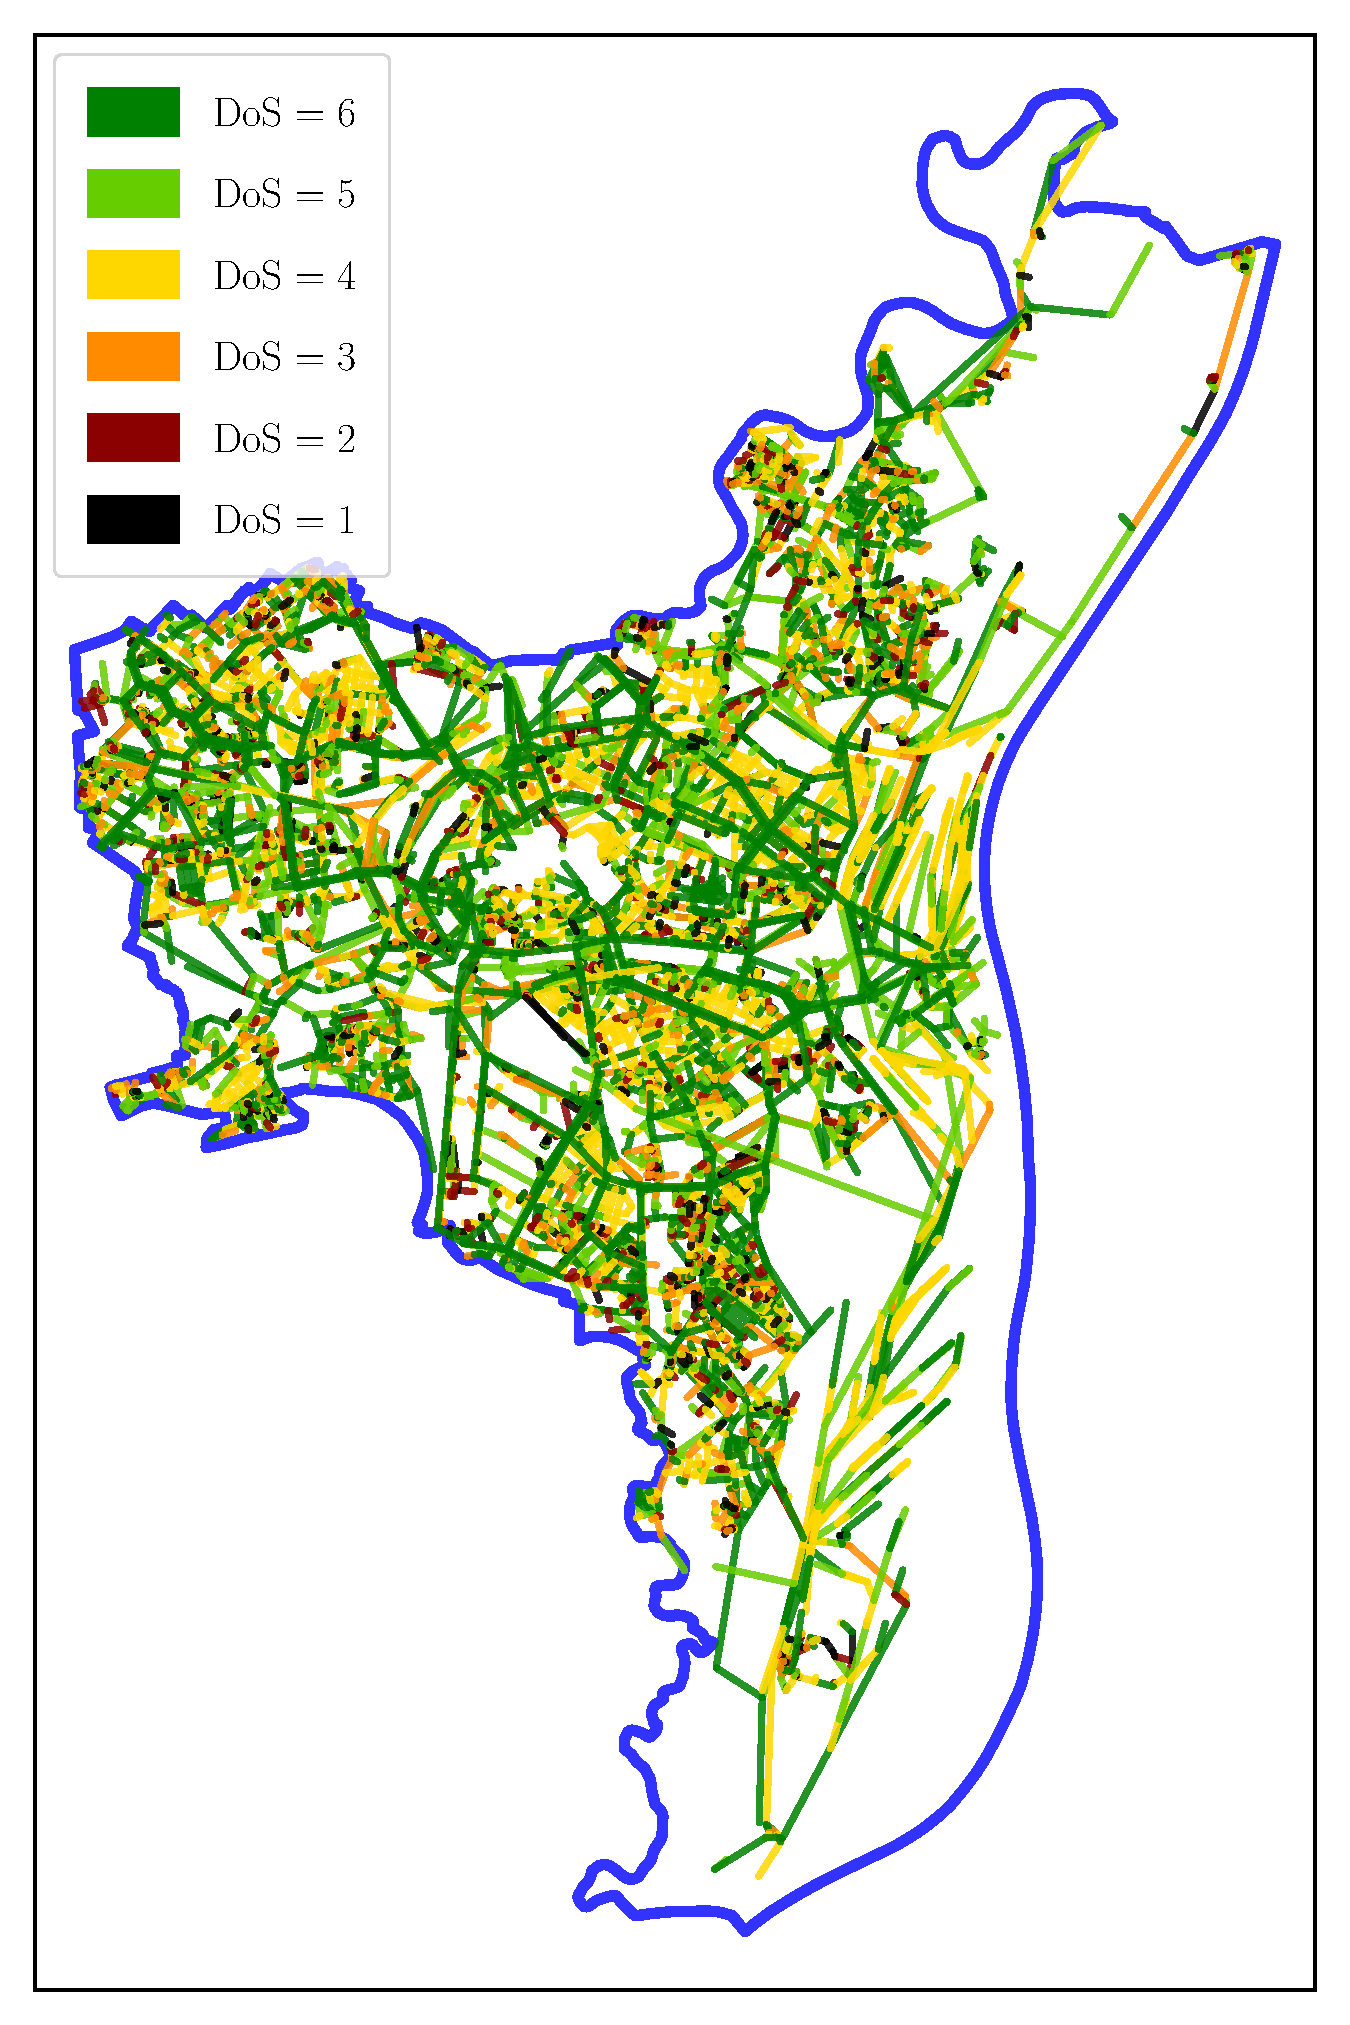
\includegraphics[width=0.48\columnwidth]{Images/GA_Stasbourg.pdf}}
\subfloat[Clustered GA lifted to original]{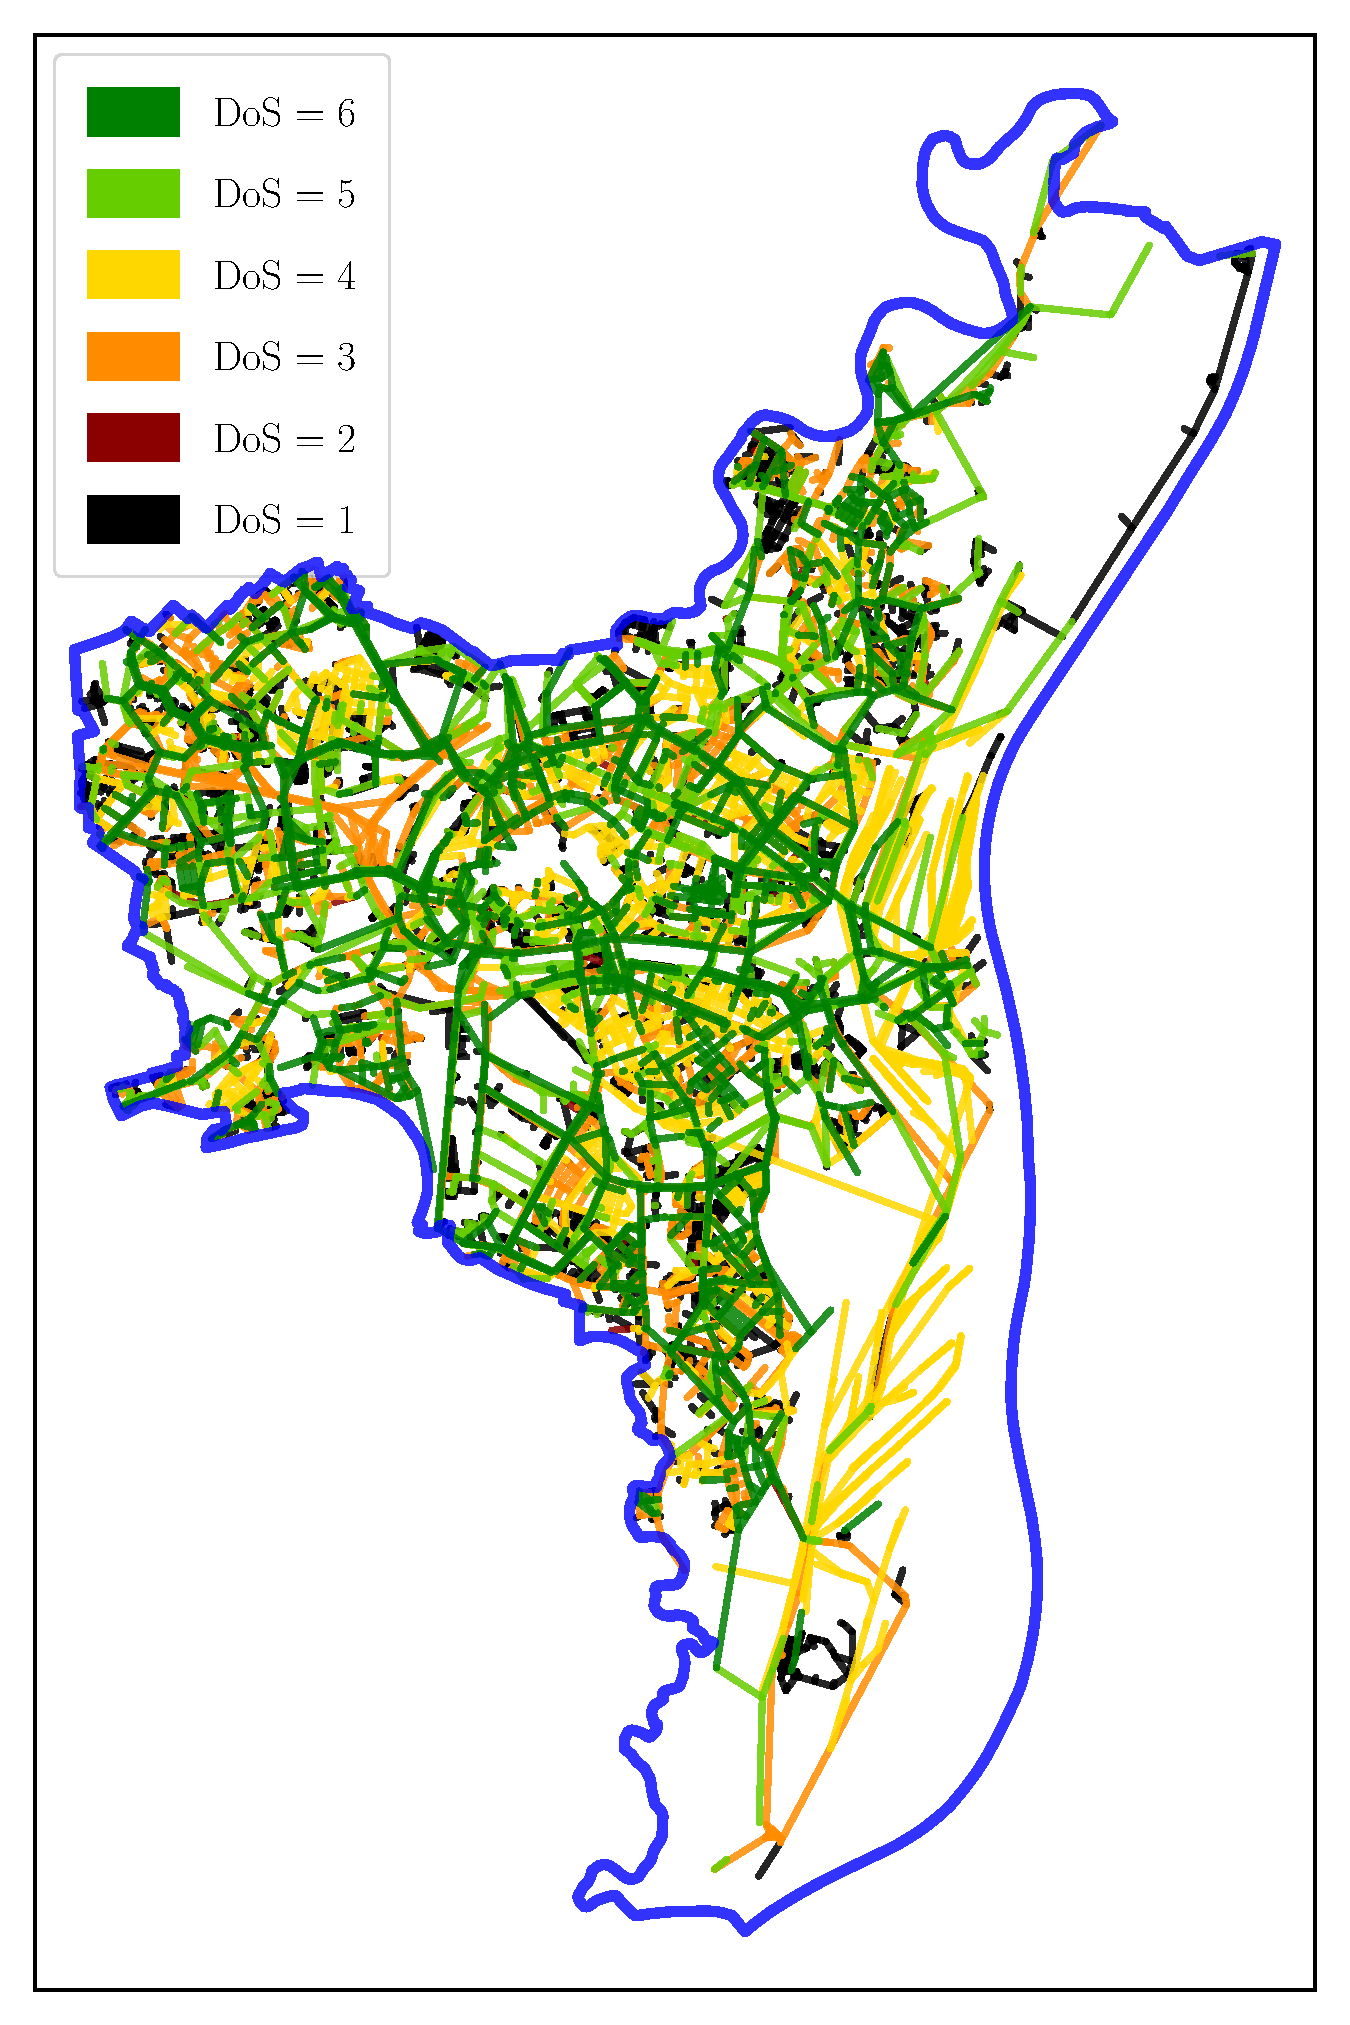
\includegraphics[width=0.48\columnwidth]{Images/Strasbourg_lift_GA_Original_2.pdf}}
\subfloat[Transferred GA Grenoble strategy lifted to original Strasbourg]
{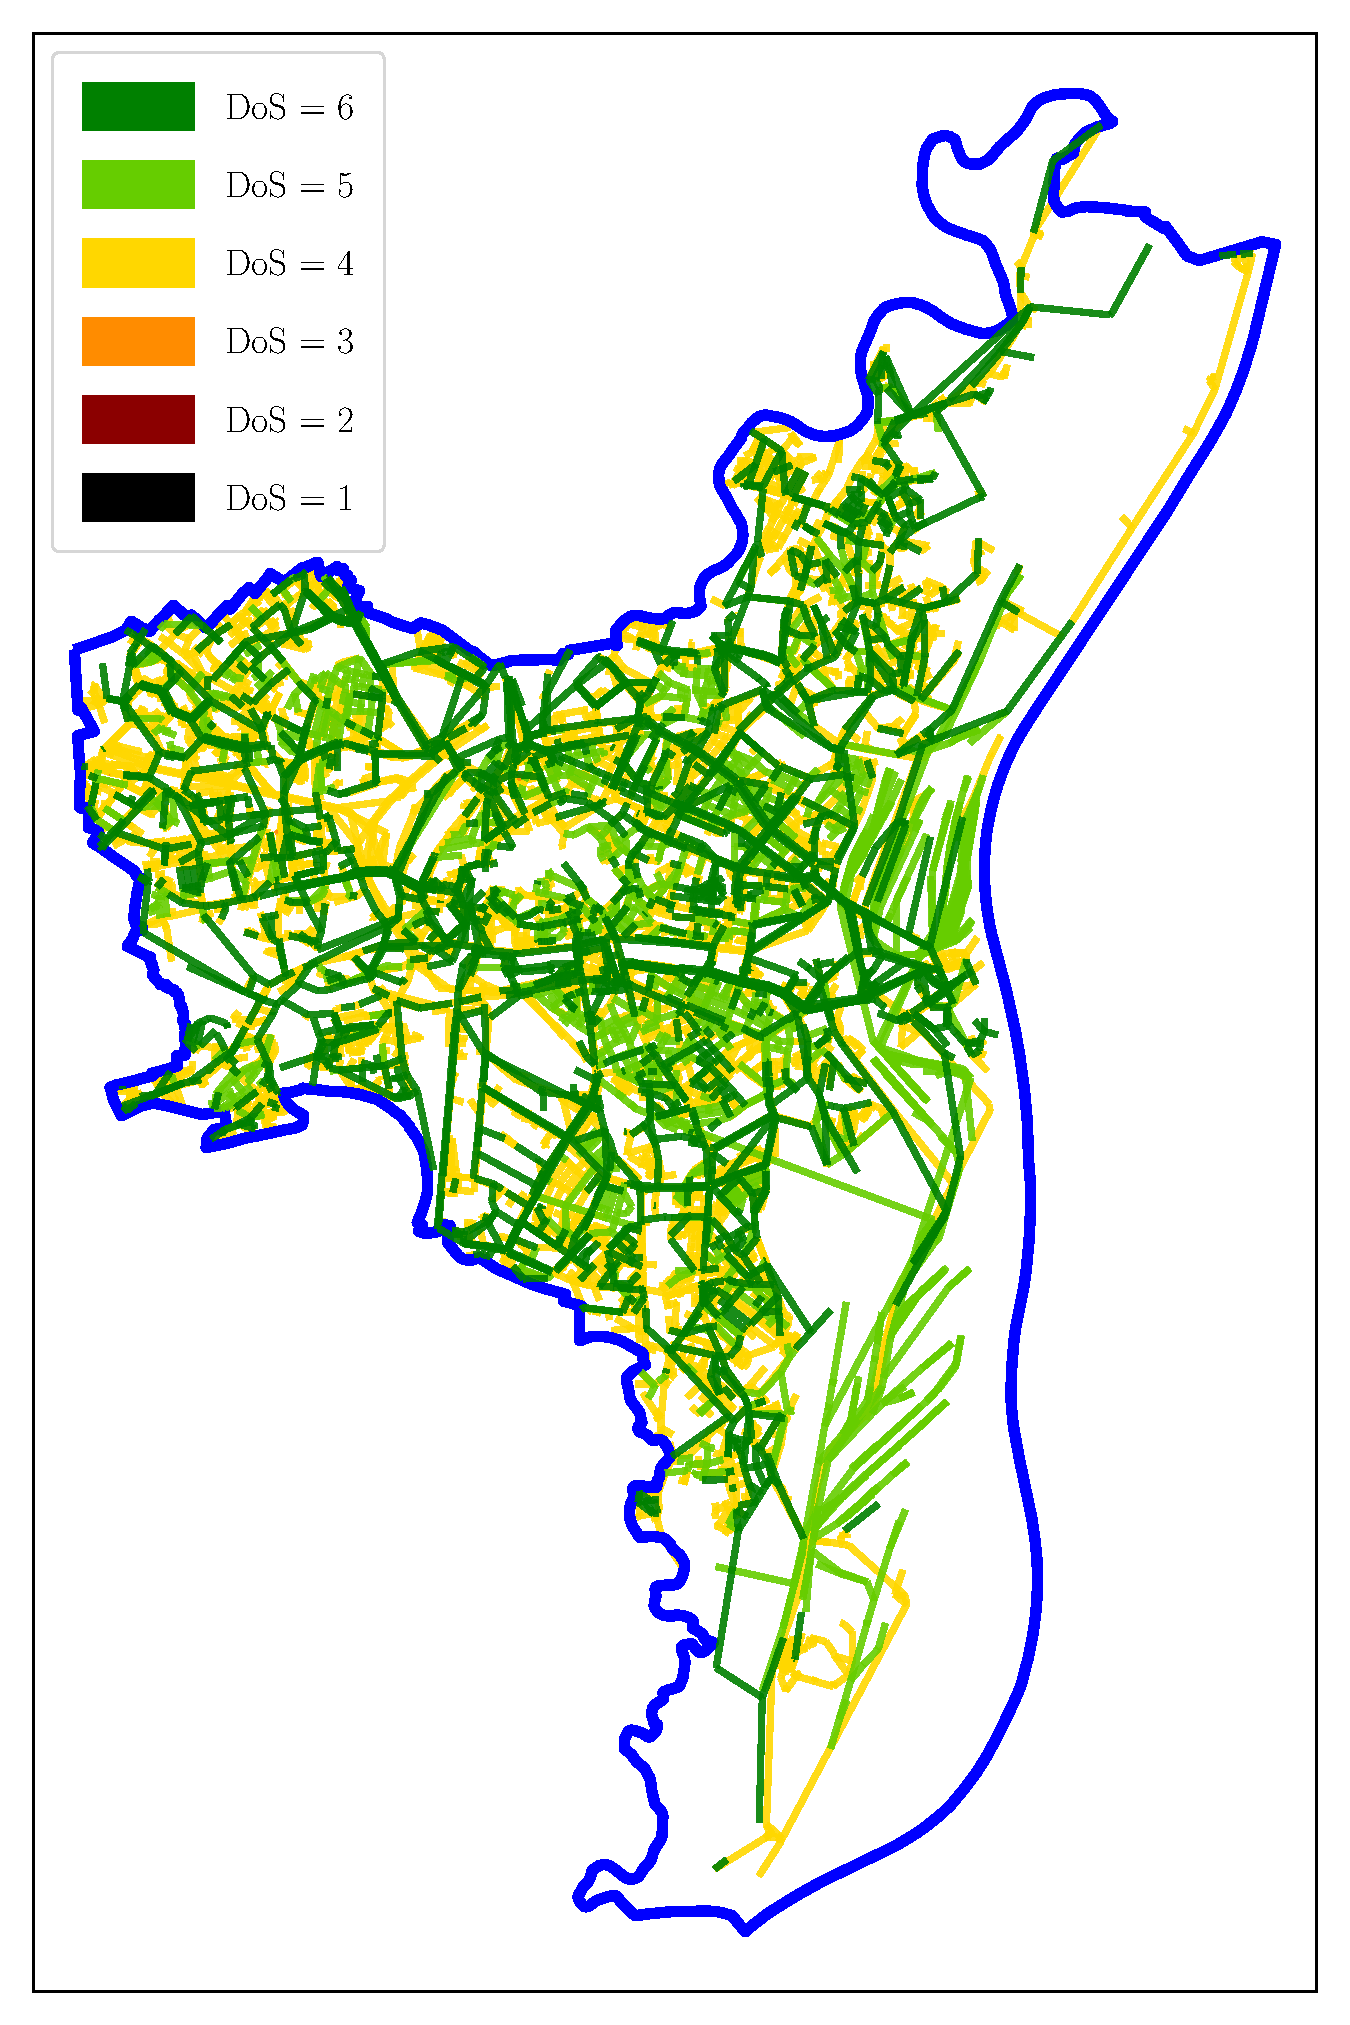
\includegraphics[width=0.480\columnwidth]{Images/transferred_clustered_on_original_geometry_strasbourg.pdf}}\\
\subfloat[Clustered Strasbourg]{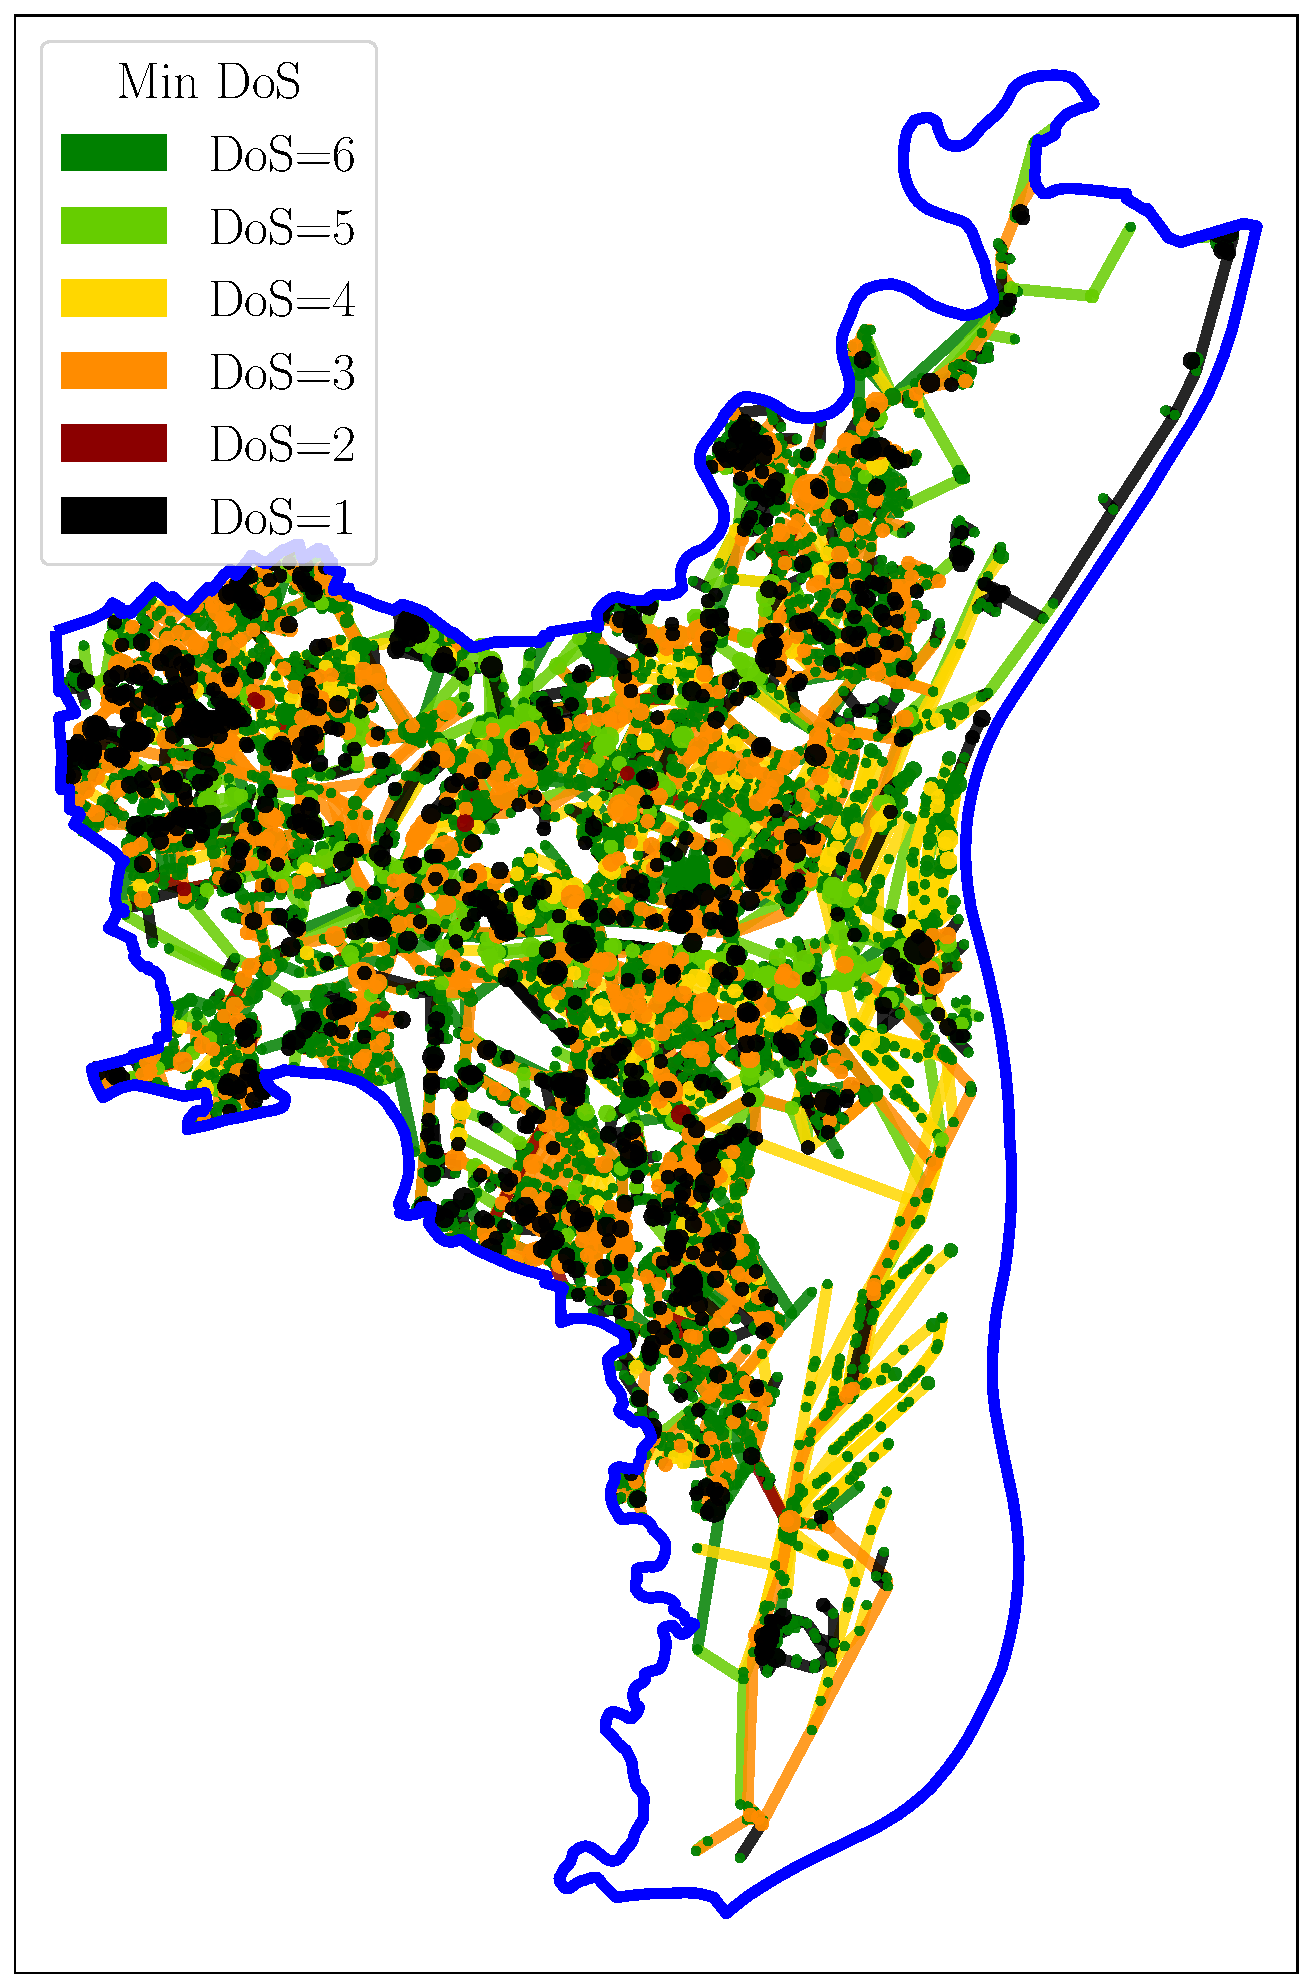
\includegraphics[width=0.48\columnwidth]{Images/clustered_dos_Strasbourg_1.pdf}}
\subfloat[GA on clustered Strasbourg]{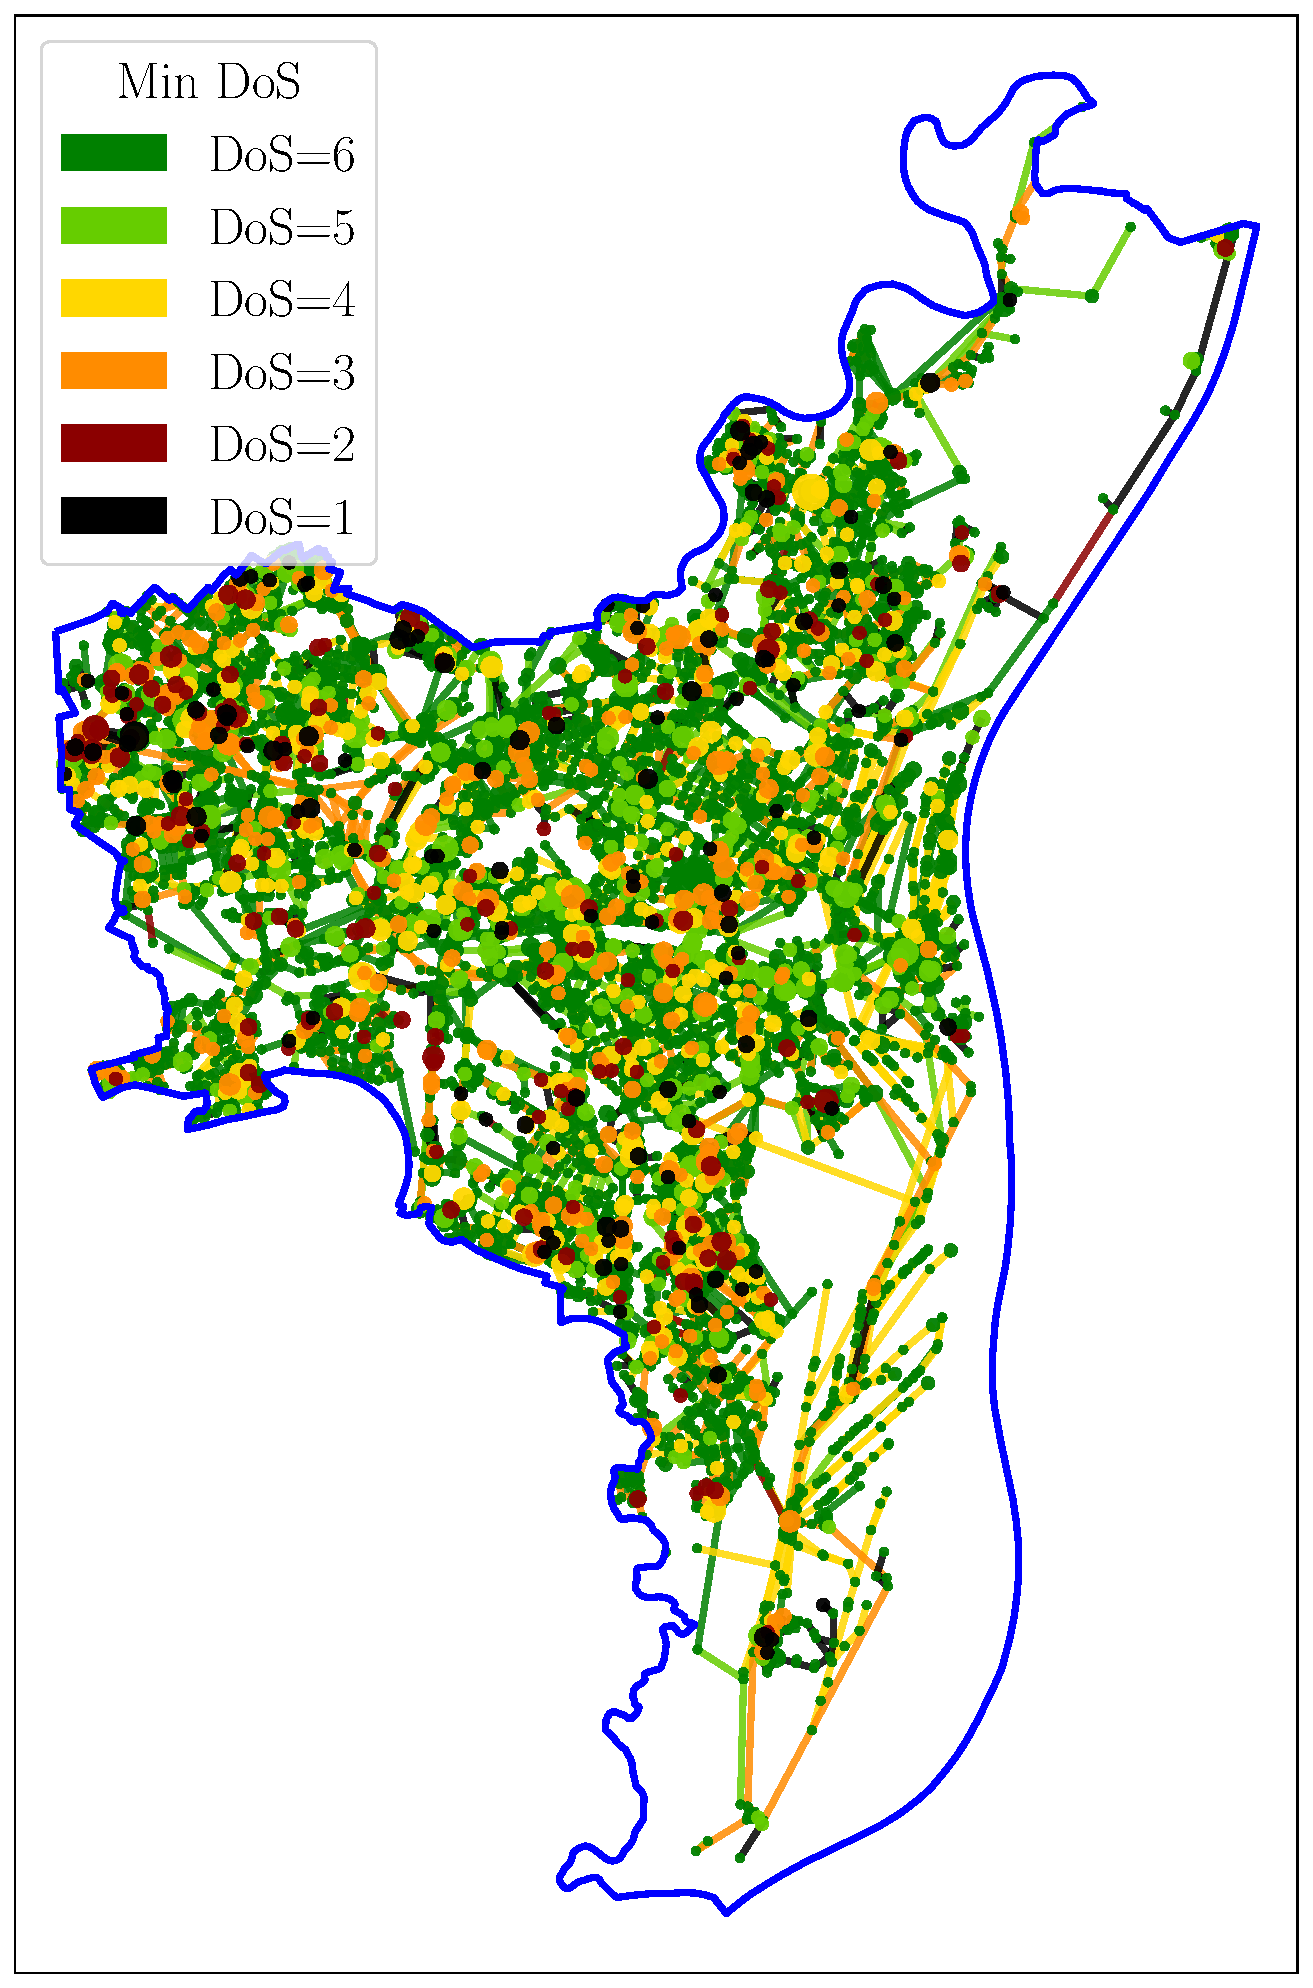
\includegraphics[width=0.48\columnwidth]{Images/optimized_clustered_dos_strasbourg.pdf}}
\subfloat[GA on Grenoble]{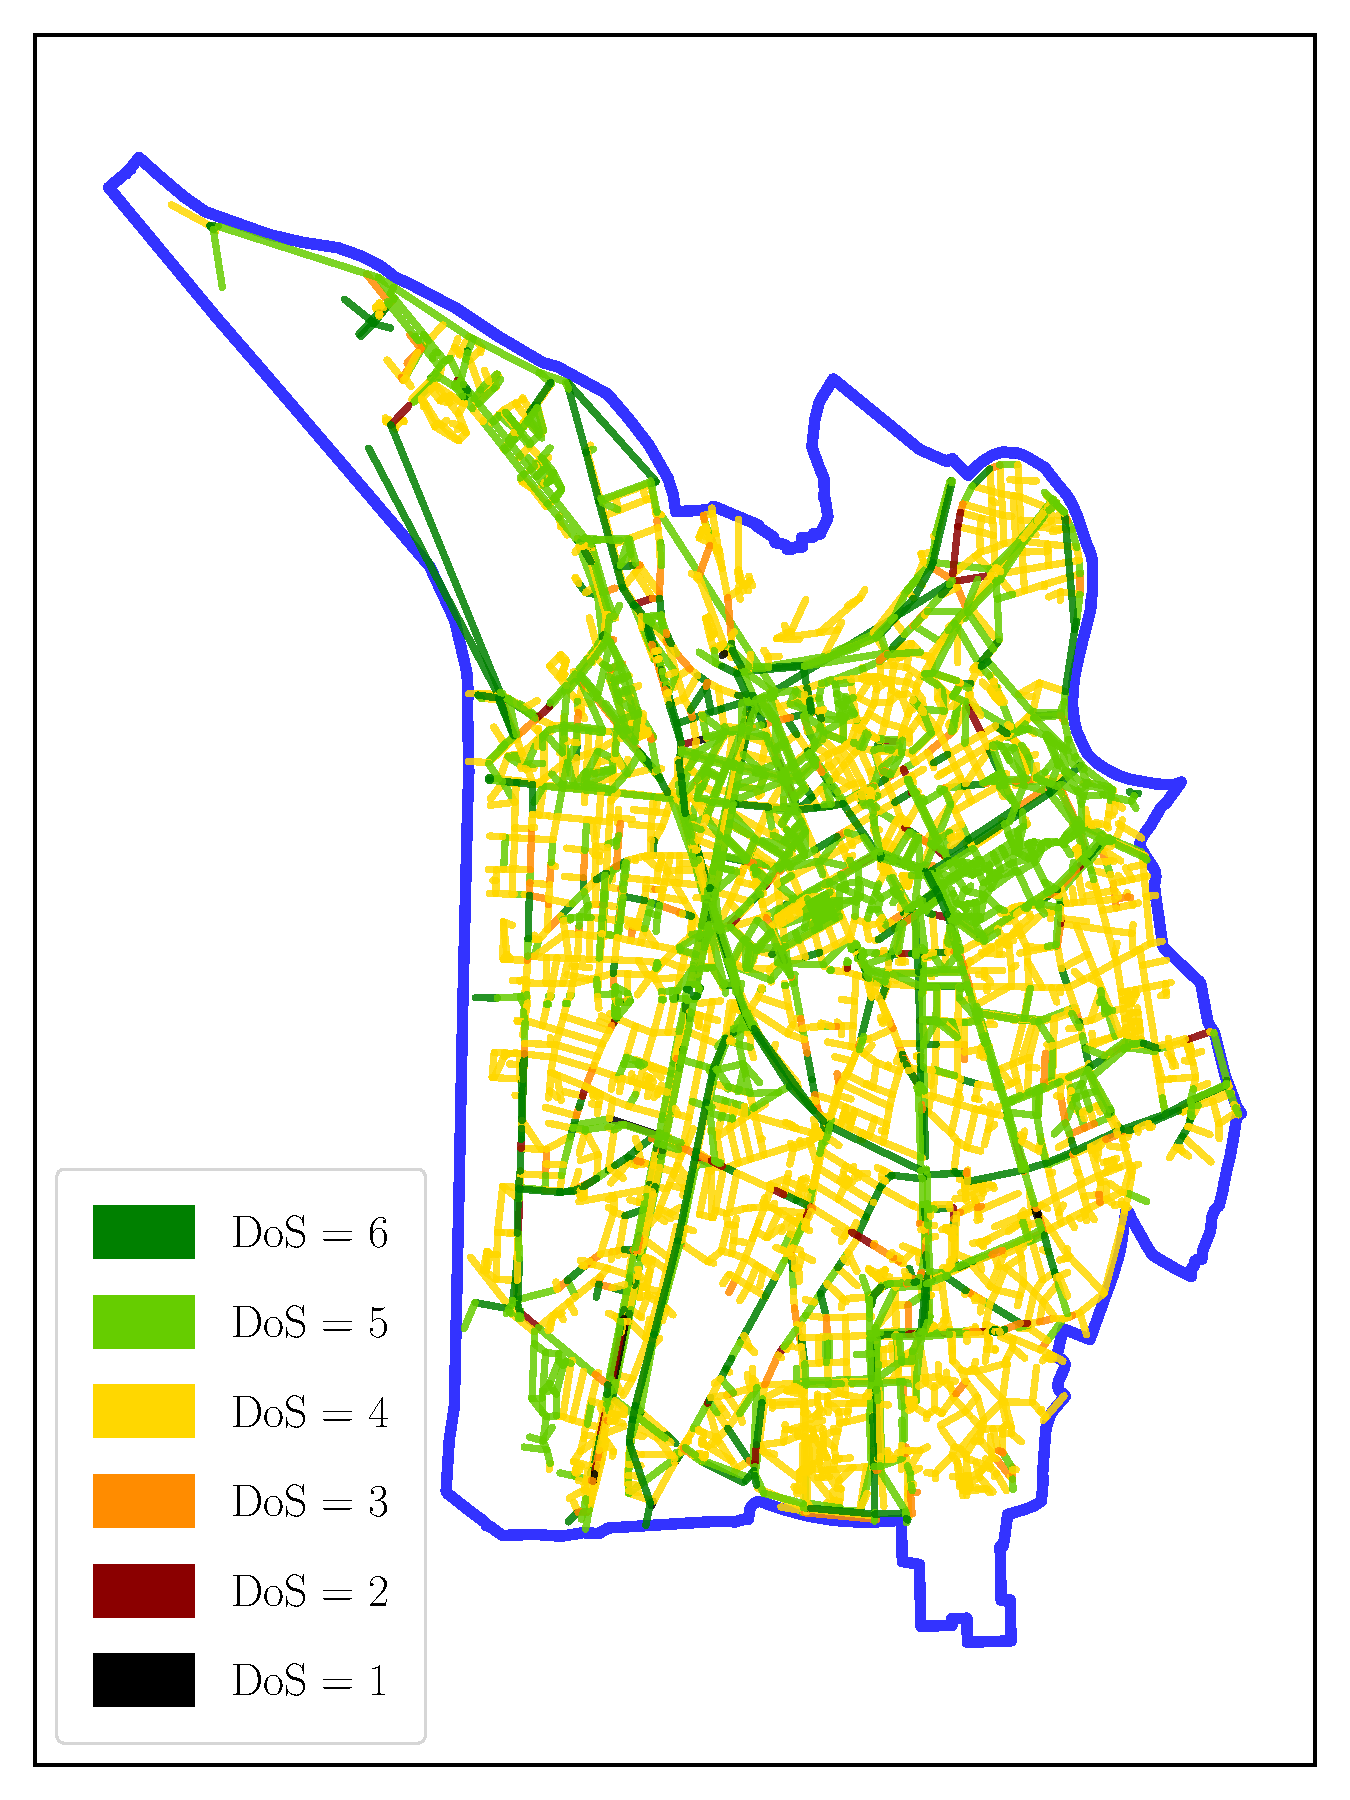
\includegraphics[width=0.48\columnwidth]{Images/Grenoble_GA.pdf}}
\subfloat[Grenoble strategy transferred to Strasbourg]{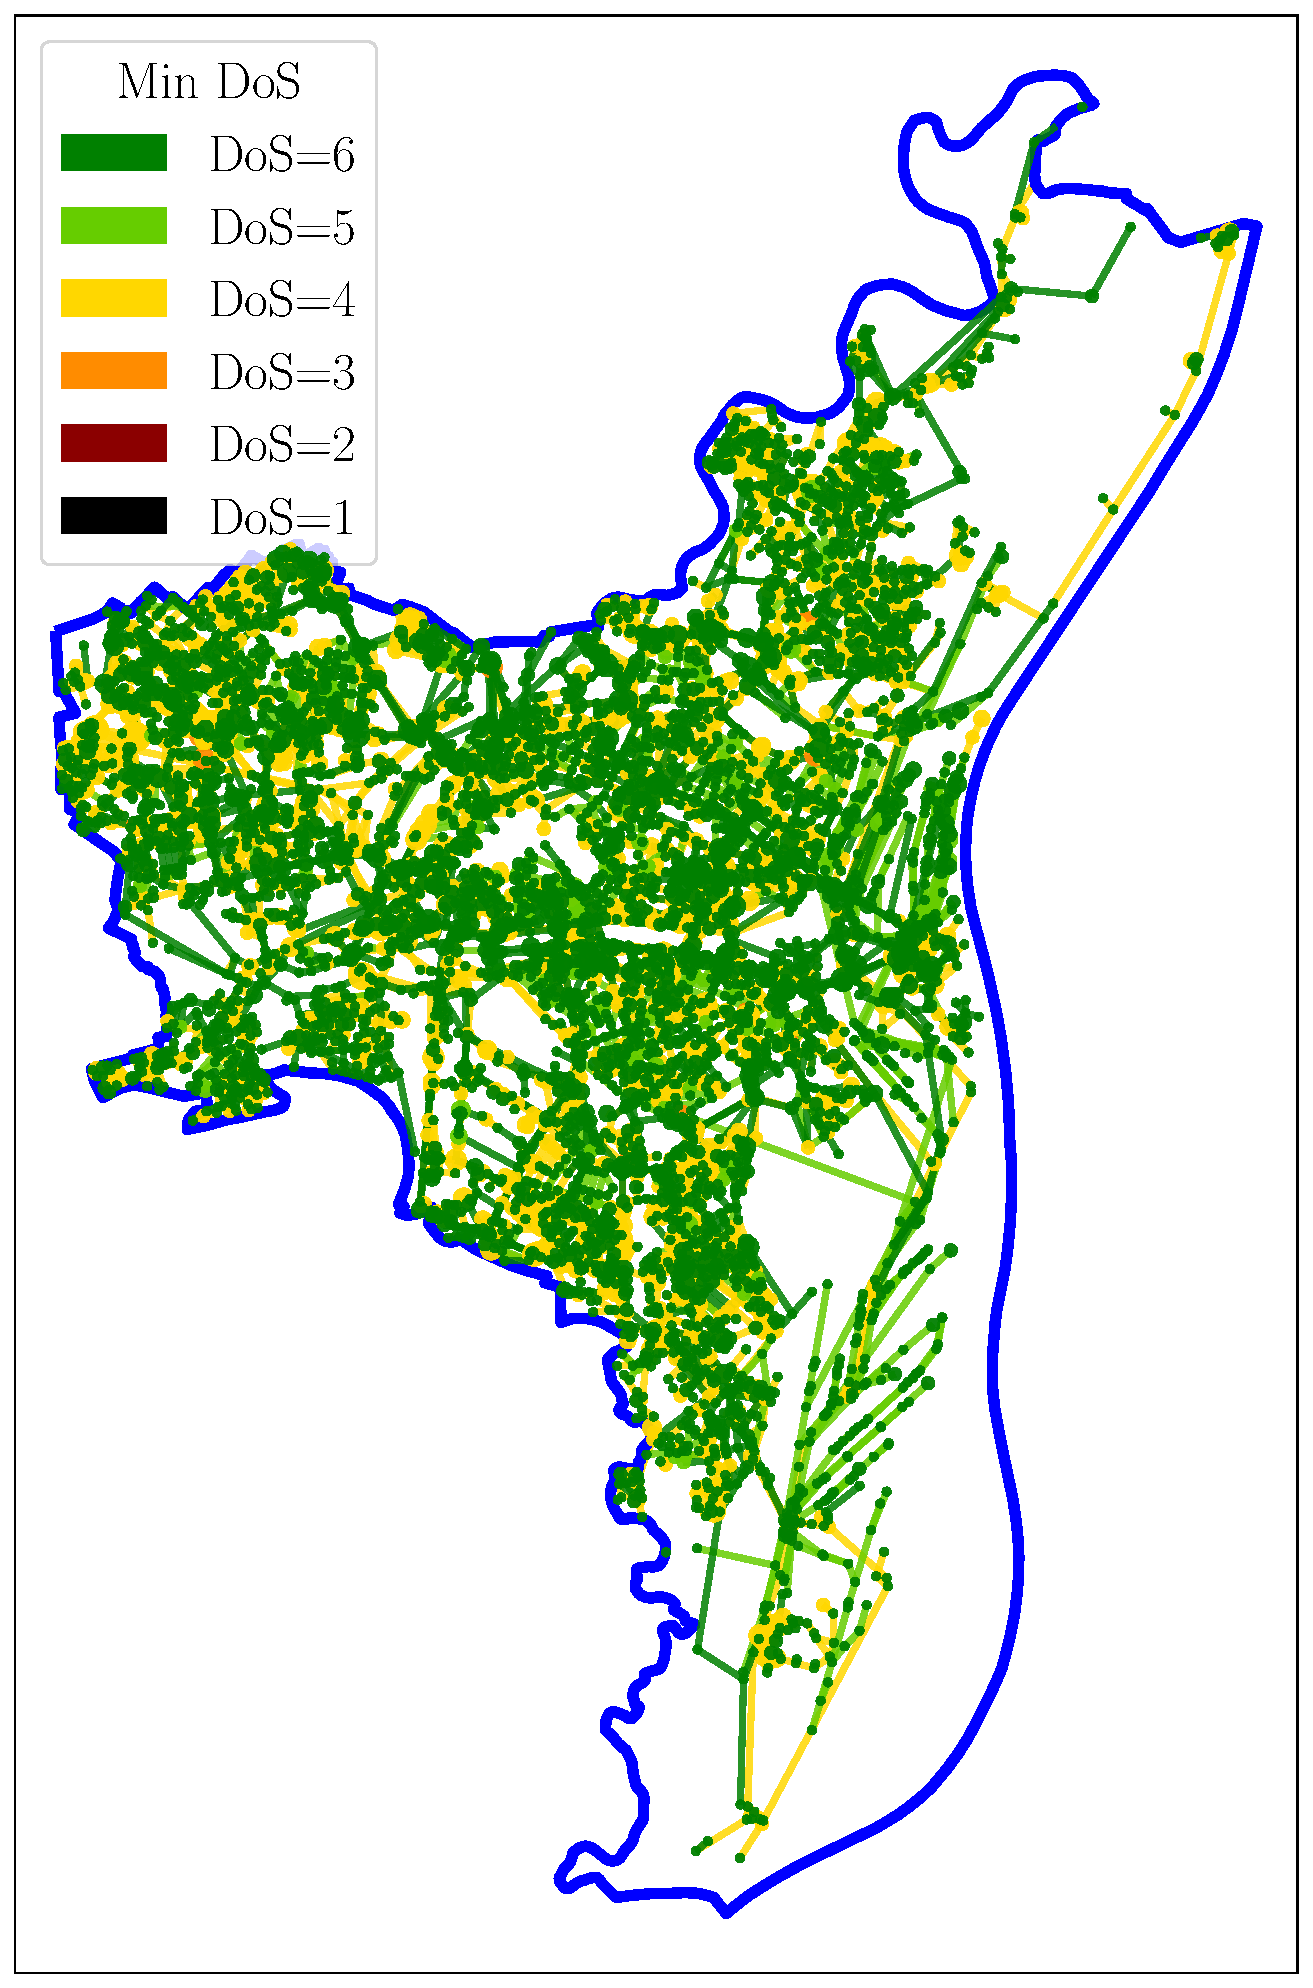
\includegraphics[width=0.48\columnwidth]{Images/transferred_clustered_dos_strasbourg.pdf}}
\caption{\footnotesize
Optimization and transfer strategies for the Strasbourg cycling network with $\beta=\frac{2}{5}$. The
first row shows arc-level configurations on the original network: (a) initial
DoS, (b) direct GA solution, (c) clustered GA solution lifted back to the
original network, and (d) Grenoble strategy transferred through the GW
correspondence and lifted to Strasbourg. The second row shows the corresponding
clustered and source-network representations: (e) clustered Strasbourg, (f) GA
solution on clustered Strasbourg, (g) GA solution on Grenoble, and (h) Grenoble
strategy transferred to Strasbourg. Colors indicate DoS levels, with lower
values corresponding to less separated cycling infrastructure.
}
\label{fig:strasbourg_optimization_transfer}
\end{figure*}




% We illustrate the proposed framework on three French cities with well-developed
% cycling networks: Lyon, Strasbourg, and Grenoble. The corresponding networks
% contain $11\,857$, $11\,417$, and $6\,773$ nodes, respectively. Since Grenoble is
% the smallest network, we use it as the reference network
% $\mathcal{H}^{\mathrm{Grenoble}}$.

% For each larger city, we apply the safety-aware clustering procedure of
% Algorithm~1 to obtain a clustered representation with the same number of nodes
% as Grenoble. Thus, Lyon and Strasbourg are reduced to clustered networks
% $\tilde{\mathcal{G}}^{\mathrm{Lyon}}$ and
% $\tilde{\mathcal{G}}^{\mathrm{Strasbourg}}$, satisfying
% \[
% |\tilde{\mathcal{V}}^{\mathrm{Lyon}}|
% =
% |\tilde{\mathcal{V}}^{\mathrm{Strasbourg}}|
% =
% |\mathcal{V}^{\mathrm{Grenoble}}|
% =
% 6\,773.
% \]
% This common resolution allows us to compare the safety-exposure structure of
% each clustered network with Grenoble using the GW distance introduced in
% Section~\ref{sec:gw_comparison}.

% We then compare three strategies: direct arc-level optimization, clustered
% optimization followed by lifting, and GW-based transfer of the optimized
% Grenoble strategy to Lyon and Strasbourg. This allows us to assess whether the
% clustered formulation preserves optimization quality and whether safety
% intervention patterns can be transferred across structurally similar cycling
% networks.

% Fig.~\ref{fig:exposure_comparison} reports the evolution of clustered
% exposure $\mathcal{E}^{\mathrm{clust}}$ and clustered flow
% $\Phi^{\mathrm{clust}}$ as the number of clusters decreases for Lyon and
% Strasbourg. The blue vertical line indicates the Grenoble resolution
% ($6\,773$ nodes), while the red line marks the point at which the clustered
% exposure begins to noticeably deviate from the original value. Compared with
% unconstrained $k$-means, CC Algorithm preserves exposure more accurately,
% especially under stronger compression. Lyon reaches the divergence threshold
% earlier, around $6\,200$ clusters, whereas Strasbourg remains stable over a
% wider range of cluster counts, suggesting that its safety structure is more
% compressible. In both cities, the clustered flow remains nearly constant under
% Algorithm~1, indicating that cyclist demand is well preserved.

% Fig.~\ref{fig:cluster_comparison_topology} provides a spatial comparison of
% the original and clustered DoS patterns. While unconstrained $k$-means can merge
% segments with very different safety levels, Algorithm~1 better preserves
% high-risk corridors and low-risk greenways by enforcing DoS consistency and
% spatial compactness. This visual agreement supports the quantitative trends in
% Figure~\ref{fig:exposure_comparison}: the constrained clustering produces
% reduced networks that remain faithful to the original safety-exposure structure.

% We next quantify cross-city similarity using the GW distance introduced in
% Section~\ref{sec:gw_comparison}. After reducing Lyon and Strasbourg to the
% Grenoble resolution, we obtain
% \begin{align*}
% GW(\mathcal{H}^{\mathrm{Grenoble}},\tilde{\mathcal{G}}^{\mathrm{Strasbourg}})
% & = 0.0085, \\
% GW(\mathcal{H}^{\mathrm{Grenoble}},\tilde{\mathcal{G}}^{\mathrm{Lyon}})
% & = 0.0243.
% \end{align*}
% The smaller distance for Strasbourg indicates that its clustered exposure
% structure is closer to Grenoble's than Lyon's is. In other words, the regions of
% high and low cyclist exposure in Strasbourg can be matched to Grenoble with less
% structural distortion.

% This result is consistent with the previous clustering analysis: Strasbourg
% showed more stable exposure under compression, and it also appears closer to
% Grenoble according to the GW comparison. Lyon, by contrast, exhibits a larger GW
% distance, suggesting a more distinct exposure-weighted network structure. These
% differences provide a useful basis for the transfer experiments below, where the
% optimized Grenoble strategy is expected to be more directly transferable to
% Strasbourg than to Lyon.

% This ordering is also coherent with external evidence from the Baromètre Vélo
% survey~\cite{parlonsvelo}, where Grenoble and Strasbourg are regularly among the
% most bicycle-friendly French cities in terms of perceived safety and comfort,
% while Lyon tends to score slightly lower. Thus, the proposed safety-aware
% comparison recovers a plausible qualitative ranking using only infrastructure,
% flow, and exposure information.

% We next evaluate the optimization and transfer strategies under different budget
% levels. Let $B_{\max}$ denote the budget required to upgrade every arc in the
% original network to the highest safety level, DoS~$6$ that is $
% B_{\max}
% =
% \sum_{a\in\mathcal{A}}
% d_a \cdot \pi(w_a^0,6).$
% The available budget is defined as $
% B=\beta \cdot B_{\max},$
% where $\beta$ is the budget fraction. We consider
% $\beta\in\{1/5,2/5,3/5,4/5\}$ in order to compare the methods under increasing
% investment levels.

% Fig.~\ref{fig:exposure_barplots} reports the normalized exposure obtained by
% the direct GA, the clustered GA lifted back to the original network, and the
% GW-based transferred solution. For both Strasbourg and Lyon, the lifted
% clustered solution remains very close to the direct GA solution across all
% budget levels. This indicates that the clustered representation preserves the
% main exposure-relevant structure needed for optimization, while substantially
% reducing the search space. The transferred strategy also follows the same
% decreasing trend as the budget increases, showing that the Grenoble solution can
% provide a meaningful intervention pattern for larger target cities.

% The results are consistent with the GW comparison above. Since Strasbourg is
% closer to Grenoble in the GW sense, its transferred solution stays closer to the
% direct and clustered GA solutions. For Lyon, where the GW distance indicates a
% less similar exposure structure, the transferred solution remains feasible and
% effective but shows a larger gap. This supports the interpretation that the GW
% metric is informative for transfer: smaller GW distances correspond to stronger
% compatibility between source and target intervention patterns.

% Fig.~\ref{fig:strasbourg_optimization_transfer} illustrates this behavior on
% the Strasbourg network for $\beta=\frac{2}{5}$. The direct GA and the lifted clustered GA produce
% visually similar improvements on the original graph, confirming that the
% clustered optimization can be lifted back without losing the main spatial
% structure of the intervention. The transferred Grenoble strategy also upgrades
% many of the same high-priority corridors, although with some differences due to
% the fact that it is guided by the source network rather than optimized directly
% on Strasbourg. Overall, the figure shows that both lifting and GW-based transfer
% produce interpretable arc-level strategies on the original network.

% Finally, the convergence and runtime results highlight the computational benefit
% of the clustered formulation. As shown in the exposure-evolution curves in Fig.~\ref{fig:algorithms_convergence}, both
% the direct GA and the lifted clustered GA reduce normalized exposure as the
% number of generations increases, but the clustered approach often reaches a
% comparable exposure level earlier, especially for the larger budget fractions.
% This suggests that optimizing on $\tilde{\mathcal{G}}$ can guide the search
% toward good intervention patterns with fewer effective iterations. The runtime curves further support this observation. The clustered GA requires
% substantially less computational time than the direct arc-level GA across the
% tested budget levels, while still producing lifted solutions that remain close
% to the direct GA in terms of final exposure. This confirms the practical value of
% the clustering-and-lifting strategy: it reduces the dimension of the
% optimization problem, accelerates convergence, and preserves most of the
% exposure-reduction benefit when the solution is evaluated back on the original
% network. Together with the transfer experiments, these results show that the
% proposed framework provides a scalable way to compare, optimize, and transfer
% cycling-infrastructure interventions across cities.

% \section{Case Study}
% \label{sec:case_study}

% We evaluate the proposed framework on three French cycling networks: Lyon
% ($11\,857$ nodes), Strasbourg ($11\,417$ nodes), and Grenoble ($6\,773$ nodes).
% Since Grenoble is the smallest network, it is used as the reference network
% $\mathcal{H}^{\mathrm{Grenoble}}$. Lyon and Strasbourg are clustered using
% Algorithm~1 so that their reduced networks,
% $\tilde{\mathcal{G}}^{\mathrm{Lyon}}$ and
% $\tilde{\mathcal{G}}^{\mathrm{Strasbourg}}$, have the same number of nodes as
% Grenoble. This common resolution enables fair GW-based comparison and
% cross-city transfer of optimization strategies.

% Figure~\ref{fig:exposure_comparison} shows that the constrained clustering
% algorithm preserves clustered exposure and flow more accurately than
% unconstrained $k$-means, especially under stronger compression. Strasbourg
% remains stable over a wider range of cluster counts, while Lyon begins to
% diverge earlier. Figure~\ref{fig:cluster_comparison_topology} confirms this
% spatially: Algorithm~1 better preserves high-risk corridors and low-risk
% greenways by enforcing DoS consistency and spatial compactness.

% Using the GW distance from Section~\ref{sec:gw_comparison}, Strasbourg is found
% to be closer to Grenoble than Lyon is, indicating a more similar
% exposure-weighted network structure. This supports the transfer experiments:
% the optimized Grenoble strategy is expected to transfer more effectively to
% Strasbourg than to Lyon. This ordering is also consistent with external
% perceptions of cycling quality reported in the Baromètre Vélo survey
% \cite{parlonsvelo}.

% We then compare three optimization strategies under budget fractions
% $\beta\in\{1/5,2/5,3/5,4/5\}$, where
% \[
% B=\beta B_{\max},
% \qquad
% B_{\max}
% =
% \sum_{a\in\mathcal{A}}
% d_a\pi(w_a^0,6).
% \]
% Figure~\ref{fig:exposure_barplots} shows that the clustered GA, after lifting
% back to the original network, achieves exposure values close to the direct
% arc-level GA for both Strasbourg and Lyon. This indicates that the clustered
% representation preserves the main information needed for optimization while
% reducing the search space. The GW-based transferred solution also reduces
% exposure as the budget increases, with stronger agreement for Strasbourg,
% consistent with its smaller GW distance to Grenoble.

% Figure~\ref{fig:strasbourg_optimization_transfer} illustrates these results on
% the Strasbourg network for $\beta=2/5$. The direct GA and the lifted clustered
% GA produce visually similar intervention patterns, while the transferred
% Grenoble strategy upgrades several comparable high-priority corridors. Finally,
% Figure~\ref{fig:algorithms_convergence} shows that the clustered GA often
% reaches comparable exposure levels in fewer generations and with substantially
% lower runtime than the direct GA. Overall, the case study demonstrates that the
% framework can compare networks, optimize infrastructure efficiently through
% clustering and lifting, and transfer intervention strategies between
% structurally similar cities.


We evaluate the proposed framework on three French cities with well-developed
cycling networks: Lyon, Strasbourg, and Grenoble. The corresponding networks
contain $11\,857$, $11\,417$, and $6\,773$ nodes, respectively. Since Grenoble is
the smallest network, it is used as the reference network
$\mathcal{H}^{\mathrm{Grenoble}}$. Lyon and Strasbourg are clustered using
CC-Algorithm to obtain reduced networks
$\tilde{\mathcal{G}}^{\mathrm{Lyon}}$ and
$\tilde{\mathcal{G}}^{\mathrm{Strasbourg}}$ with the same number of nodes as
Grenoble:
\[
|\tilde{\mathcal{V}}^{\mathrm{Lyon}}|
=
|\tilde{\mathcal{V}}^{\mathrm{Strasbourg}}|
=
|\mathcal{V}^{\mathrm{Grenoble}}|
=
6\,773.
\]
This common resolution allows us to compare safety-exposure structures across
cities using the GW distance and to test whether optimized intervention
strategies can be transferred between structurally similar networks.

Fig.~\ref{fig:exposure_comparison} evaluates the quality of the clustering
step by tracking clustered exposure $\mathcal{E}^{\mathrm{clust}}$ and clustered
flow $\Phi^{\mathrm{clust}}$ as the number of clusters decreases. Compared with
unconstrained $k$-means, Algorithm~1 better preserves exposure and flow,
especially under stronger compression. Strasbourg remains stable over a wider
range of cluster counts, while Lyon begins to deviate earlier, suggesting that
Strasbourg's safety-exposure structure is more easily compressed. The spatial
comparison in Fig.~\ref{fig:cluster_comparison_topology} supports this result:
the constrained clustering better preserves high-risk corridors and low-risk
greenways by enforcing DoS consistency and spatial compactness.

After clustering, we compare Lyon and Strasbourg with Grenoble using the
GW distance introduced in Section~\ref{sec:gw_comparison}. The results indicate
that Strasbourg is closer to Grenoble than Lyon is in terms of exposure-weighted
network structure. This is consistent with the previous compression results and
suggests that the optimized Grenoble strategy should be more transferable to
Strasbourg. The ordering also agrees with external evidence from the
Baromètre Vélo survey~\cite{parlonsvelo}, where Grenoble and Strasbourg are
typically ranked among the most bicycle-friendly French cities, while Lyon tends
to score slightly lower.

We then evaluate three optimization strategies: direct arc-level GA optimization,
clustered GA optimization followed by lifting, and GW-based transfer of the
optimized Grenoble strategy. The available budget is defined as a fraction of
the maximum budget required to upgrade all arcs to DoS~$6$:$
B=\beta \cdot B_{\max},
\qquad
B_{\max}
=
\sum_{a\in\mathcal{A}}
d_a \cdot \pi(w_a^0,6)$,
with $
\beta\in\left\{\frac{1}{5},\frac{2}{5},\frac{3}{5},\frac{4}{5}\right\}$.
Fig.~\ref{fig:exposure_barplots} shows that the lifted clustered solution
closely follows the direct GA solution for both Lyon and Strasbourg across the
tested budget levels. This confirms that the clustered representation preserves
the main information needed for optimization while reducing the search space.
The transferred Grenoble solution also reduces exposure as the budget increases,
with a smaller gap for Strasbourg, which is consistent with its stronger GW
similarity to Grenoble.

Fig.~\ref{fig:strasbourg_optimization_transfer} illustrates these effects on
the Strasbourg network for $\beta=2/5$. The direct GA and lifted clustered GA
produce similar spatial intervention patterns on the original graph, showing
that clustered optimization can be lifted back without losing the main structure
of the solution. The transferred Grenoble strategy also upgrades several
comparable high-priority corridors, although it differs from the direct
Strasbourg solution because it is guided by the source network. This highlights
the interpretability of both the clustering-and-lifting strategy and the
GW-based transfer mechanism.

Finally, Fig.~\ref{fig:algorithms_convergence} compares convergence and
runtime. The lifted clustered GA reaches exposure levels close to the direct GA,
often with faster convergence, and requires substantially less computational
time. This demonstrates the practical benefit of solving the optimization problem
on $\tilde{\mathcal{G}}$ and lifting the solution back to the original network.
Overall, the case study shows that the proposed framework can compress large
cycling networks while preserving safety-relevant structure, optimize
infrastructure upgrades efficiently, and transfer intervention strategies across
cities when their exposure-weighted structures are sufficiently similar.

\section{Strengths and Limitations}
\label{sec:strengths_limitations}

The proposed framework provides a unified approach to compare, compress,
optimize, and transfer cycling-network intervention strategies using
safety-relevant quantities such as DoS, cyclist flow, traffic exposure, slope,
and angular change. Its main advantage is that the clustered representation
reduces the optimization dimension while preserving the main exposure and flow
structure of the original network. As a result, lifted clustered solutions can
remain close to direct arc-level GA solutions while requiring lower
computational cost. In addition, the GW-based comparison offers an interpretable
measure of cross-city similarity and a principled basis for transferring
optimized strategies between structurally similar networks.

The framework also has limitations. Its performance depends on the quality of
the input data, including DoS classification, traffic estimates, OD demand, and
slope information. The AON assignment is tractable but does not capture
heterogeneous cyclist preferences, stochastic route choice, or behavioral
adaptation after infrastructure changes. Moreover, clustering remains an
approximation: even though the lifting step preserves a minimum target DoS for
the original arcs, some local details inside clusters may be smoothed. Finally,
the transfer procedure assumes that GW similarity is a useful proxy for
intervention transferability, an assumption that should be further tested on a
larger set of cities.

\section{Conclusions and Future Work}
\label{sec:conclusion}

This paper introduced a safety-aware framework for comparing and optimizing
cycling networks across cities. The method combines exposure-based network
metrics, constrained clustering, bi-level infrastructure optimization, and
GW-based transfer of upgrade strategies. By clustering larger networks to the
same resolution as a reference city, the framework enables fair cross-city
comparison while reducing the optimization search space. The case study on
Grenoble, Strasbourg, and Lyon shows that clustered optimization can be lifted
back to the original network with competitive exposure reductions and lower
runtime, while the transfer results suggest that cities with smaller GW
distances share more compatible intervention patterns.

Future work will focus on richer route-choice models that capture heterogeneous
and stochastic cyclist behavior, and on clustering constraints that incorporate
equity, accessibility~\cite{jurado2025transport}, and connectivity to key urban
facilities~\cite{jurado2025improving}. The transfer methodology should also be
tested on more cities to better identify when optimized strategies generalize
across networks. Finally, the optimization model could be extended to
multi-objective settings that jointly consider exposure reduction, cost,
coverage, equity, and implementation feasibility.

% \section{Strengths and Limitations}
% \label{sec:strengths_limitations}

% The proposed framework has several strengths. First, it provides a unified way to
% compare, compress, optimize, and transfer cycling-network intervention
% strategies using safety-relevant quantities such as DoS, cyclist flow, traffic
% exposure, slope, and angular change. Second, the clustered representation reduces
% the size of the optimization problem while preserving the main exposure and flow
% structure of the original network. This makes it possible to obtain lifted
% solutions that remain close to the direct arc-level GA solutions, but with lower
% computational cost. Third, the GW-based comparison provides an interpretable
% measure of cross-city similarity and offers a principled basis for transferring
% optimized strategies from a source network to a structurally similar target
% network.

% There are also limitations. The quality of the framework depends on the accuracy
% of the input data, including the DoS classification, traffic estimates, OD
% demand, and slope information. The AON assignment provides a simple and
% tractable model of cyclist route choice, but it does not capture heterogeneous
% preferences, stochastic route choice, or behavioral adaptation after
% infrastructure changes. The clustered optimization is an approximation: although
% the lifting step preserves a minimum target DoS for the original arcs, local
% details inside clusters may still be smoothed. Finally, the transfer procedure
% assumes that structural similarity, as measured by the GW distance, is a useful
% proxy for intervention transferability. The results support this assumption in
% the case study, but broader validation on more cities is needed.

% \section{Conclusions and Future Work}
% \label{sec:conclusion}

% This paper introduced a safety-aware framework for comparing and optimizing
% cycling networks across cities. The method combines exposure-based network
% metrics, constrained clustering, bi-level infrastructure optimization, and
% GW-based transfer of upgrade strategies. By clustering larger networks to the
% same resolution as a reference city, the framework enables fair cross-city
% comparison while reducing the dimension of the optimization problem. The case
% study on Grenoble, Strasbourg, and Lyon shows that the clustered optimization can
% be lifted back to the original network with competitive exposure reductions and
% substantially lower computational time. The transfer results further suggest
% that cities with smaller GW distances can share more compatible intervention
% patterns, supporting the use of safety-aware network similarity as a guide for
% cross-city planning.

% Future work will extend the framework in several directions. First, richer route
% choice models could be incorporated to account for heterogeneous cyclist
% preferences and stochastic behavior. Second, the clustering procedure could be
% adapted to include additional constraints, such as equity, accessibility \cite{jurado2025transport}, or
% connectivity to key urban facilities \cite{jurado2025improving}. Third, the transfer methodology should be
% tested on a larger set of cities to better understand when optimized strategies
% generalize across networks. Finally, the optimization model could be extended to
% multi-objective settings that jointly consider exposure reduction, cost,
% coverage, equity, and implementation feasibility.

% \section*{APPENDIX A}
% \subsection*{Complementary Proofs}
% \textbf{Theorem} 1 affirms that matrix $\mathcal{L} = I - D^{-1/2}AD^{-1/2}$ is a valid symmetric normalized graph Laplacian.

% \begin{proof}
% The proof follows from the symmetry and non-negativity of the adjacency matrix $A$ and the subsequent definition of $\mathcal{L}$.


%     \textit{$i)$ Symmetry of $A$:} Although $\mathcal{G}$ is directed, the arc attributes are symmetric:
% \[
% w_{(u,v)} = w_{(v,u)},\quad
% d_{(u,v)} = d_{(v,u)},\quad
% \phi_{(u,v)} = \phi_{(v,u)}.
% \]
% Since $A_{ij}$ is defined as a nonnegative function of $(w_{ij}, d_{ij}, \phi_{ij})$
% with no directional bias, it follows that $A_{ij}~=~A_{ji}$ and hence $A = A^\top$.

%     \textit{$ii)$ Non-negativity of $A$:} By definition, $w_{ij} \geq 0$, $d_{ij} \geq 0$, $\phi_{ij} \geq 0$, $\max(\boldsymbol{\phi}) > 0$, and the exponential function is always positive. Therefore, for all $(i,j) \in \mathcal{A}$, $A_{ij} \geq 0$. For non-adjacent nodes, $A_{ij} = 0$ by definition.

%      \textit{$iii)$ Properties of $\mathcal{L}$:}
%      Consider the (unnormalized) Laplacian $L = D - A$. For any
% $\mathbf{y} \in \mathbb{R}^{|\mathcal{V}|}$,
% \[
% \mathbf{y}^\top L \mathbf{y}
% = \frac{1}{2} \sum_{i,j} A_{ij} (y_i - y_j)^2 \;\geq\; 0,
% \]
% so $L$ is positive semidefinite. The normalized Laplacian can be written as
% \[
% \mathcal{L} \;=\; D^{-1/2} L D^{-1/2}.
% \]
% For any $\mathbf{x}$, let $\mathbf{y} = D^{-1/2} \mathbf{x}$. Then
% \[
% \mathbf{x}^\top \mathcal{L} \mathbf{x}
% = (D^{-1/2}\mathbf{x})^\top L (D^{-1/2}\mathbf{x})
% = \mathbf{y}^\top L \mathbf{y} \;\geq\; 0,
% \]
% which shows that $\mathcal{L}$ is positive semidefinite. Since
% $\mathcal{L}$ is also symmetric, all its eigenvalues are real and
% nonnegative (and, by standard results, lie in $[0,2]$). This completes the proof.

% \end{proof}

% \textbf{Theorem} 2 guarantees  that given a di-graph $\mathcal{G} = (\mathcal{V}, \mathcal{A}, \mathcal{W})$ with demand matrix $q_{(u,v)}$ and its clustered representation $\tilde{\mathcal{G}} = (\tilde{\mathcal{V}}, \tilde{\mathcal{A}}, \tilde{\mathcal{W}})$ constructed via Algorithm~\ref{alg:constrained-clustering-math}, the total network flow is preserved:
% \[
% \Phi^{\text{orig}} \triangleq \sum_{a \in \mathcal{A}} \phi_a
% = \sum_{\tilde{a} \in \tilde{\mathcal{A}}} \tilde{\phi}_{\tilde{a}}
% = \Phi^{\text{clust}}.
% \]

% \begin{proof}
% Observe that the clustered demand $\tilde{q}_{(C_{r},C_{r'})}$ in \eqref{cluster_demand} aggregates all original demands between nodes in clusters $C_{r}$ and $C_{r'}$ as
% \[
% \tilde{q}_{(C_{r},C_{r'})}
% =
% \sum_{\substack{u \in C_{r} \\ v \in C_{r'}}} q_{(u,v)},
% \]
% ensuring total demand preservation
% \[
% \sum_{u,v \in \mathcal{V}} q_{(u,v)}
% =
% \sum_{C_{r},C_{r'} \in \tilde{\mathcal{V}}} \tilde{q}_{(C_{r},C_{r'})}.
% \]
% In the original graph $\mathcal{G}$, the all-or-nothing assignment \eqref{eq_flows} yields arc flows
% \[
% \phi_a = \sum_{u,v} q_{(u,v)} \cdot \mathbb{I}_{a \in p_{(u,v)}},
% \]
% while in the clustered graph $\tilde{\mathcal{G}}$, \eqref{eq_cluster_flow_inter} gives clustered-arc flows
% \[
% \tilde{\phi}_{\tilde{a}}
% =
% \sum_{C_{r},C_{r'}} \tilde{q}_{(C_{r},C_{r'})} \cdot
% \mathbb{I}_{\tilde{a} \in \tilde{p}_{(C_{r},C_{r'})}}.
% \]
% The total flow in $\mathcal{G}$ decomposes as:
% \begin{align}
% \Phi^{\text{orig}}
% &= \sum_{a \in \mathcal{A}} \phi_a
% = \sum_{u,v} q_{(u,v)} \underbrace{\sum_{a \in \mathcal{A}} \mathbb{I}_{a \in p_{(u,v)}}}_{=1} \\
% &= \sum_{u,v} q_{(u,v)},
% \end{align}
% since each path $p_{(u,v)}$ covers exactly one set of arcs. Similarly, for $\tilde{\mathcal{G}}$:
% \begin{align}
% \Phi^{\text{clust}}
% &= \sum_{\tilde{a} \in \tilde{\mathcal{A}}} \tilde{\phi}_{\tilde{a}}
% = \sum_{C_{r},C_{r'}} \tilde{q}_{(C_{r},C_{r'})}
%    \underbrace{\sum_{\tilde{a} \in \tilde{\mathcal{A}}}
%                \mathbb{I}_{\tilde{a} \in \tilde{p}_{(C_{r},C_{r'})}}}_{=1} \\
% &= \sum_{C_{r},C_{r'}} \tilde{q}_{(C_{r},C_{r'})},
% \end{align}
% where the indicator sums equal 1 because each clustered path
% $\tilde{p}_{(C_{r},C_{r'})}$ traverses exactly one sequence of clustered-arcs.
% By demand conservation, we conclude
% $\Phi^{\text{orig}} \equiv \Phi^{\text{clust}}$.
% \end{proof}

\section*{APPENDIX A}
\subsection*{Complementary Proofs}

\begin{proof}[Proof of Theorem~\ref{thm:symmetry}]
The adjacency matrix $A$ is symmetric because the arc attributes used to define
it are symmetric, namely
\[
w_{(u,v)}^0=w_{(v,u)}^0,\qquad
d_{(u,v)}=d_{(v,u)},\qquad
\phi_{(u,v)}=\phi_{(v,u)}.
\]
Moreover, all terms entering $A_{ij}$ are non-negative, and $A_{ij}=0$ whenever
$(i,j)\notin\mathcal{A}$. Hence, $A=A^\top$ and $A$ is non-negative.

Let $D$ be the diagonal degree matrix and $L=D-A$ the unnormalized Laplacian.
For any $\mathbf{y}\in\mathbb{R}^{|\mathcal{V}|}$,
\[
\mathbf{y}^{\top}L\mathbf{y}
=
\frac{1}{2}
\sum_{i,j}A_{ij}(y_i-y_j)^2
\geq 0,
\]
so $L$ is positive semidefinite. Since
\[
\mathcal{L}
=
I-D^{-1/2}AD^{-1/2}
=
D^{-1/2}LD^{-1/2},
\]
it follows that, for any $\mathbf{x}$,
\[
\mathbf{x}^{\top}\mathcal{L}\mathbf{x}
=
(D^{-1/2}\mathbf{x})^{\top}
L
(D^{-1/2}\mathbf{x})
\geq 0.
\]
Therefore, $\mathcal{L}$ is symmetric positive semidefinite and is a valid
symmetric normalized graph Laplacian.
\end{proof}

\begin{proof}[Proof of Theorem~\ref{thm:flow_preservation}]
The clustered demand is defined by aggregating all OD demands between nodes
belonging to the corresponding clusters:
\[
\tilde{q}_{(C_r,C_{r'})}
=
\sum_{\substack{u\in C_r\\ v\in C_{r'}}}
q_{(u,v)}.
\]
Therefore, total demand is preserved:
\[
\sum_{u,v\in\mathcal{V}}q_{(u,v)}
=
\sum_{C_r,C_{r'}\in\tilde{\mathcal{V}}}
\tilde{q}_{(C_r,C_{r'})}.
\]
The AON assignment sends each OD demand to exactly one shortest path in the
original network and each clustered OD demand to exactly one shortest path in
the clustered network. Hence, clustering redistributes the same total demand
over aggregated paths, without creating or removing cyclist demand. Consequently,
the total assigned flow mass is preserved:
\[
\Phi^{\mathrm{orig}}
=
\sum_{u,v\in\mathcal{V}}q_{(u,v)}
=
\sum_{C_r,C_{r'}\in\tilde{\mathcal{V}}}
\tilde{q}_{(C_r,C_{r'})}
=
\Phi^{\mathrm{clust}}.
\]
\end{proof}


\section*{APPENDIX B}
Now we present the Pseudo-Code of CC-Algorithm and Solution Algorithm for Problem~\ref{bi-levelcluster}- 
\begin{algorithm}[t]
\caption{Constrained Spectral Clustering for Bike Networks (CC-Algorithm)}
\label{alg:constrained-clustering-math}
\begin{algorithmic}[1]
\Require$\mathcal{G} = (\mathcal{V}, \mathcal{A}, \mathcal{W})$, 
  $k$,
  $\epsilon_{\max}$, 
  $\delta_{\max}$, 
  $\tau_{\mathcal{E}}^{(0)}$, $\tau_{\Phi}^{(0)}$, 
  $\alpha_{\text{relax}}$, 
  $\lambda_1,\lambda_2$, 
  $T_{\max}$.
\Ensure $\tilde{\mathcal{G}} = (\tilde{\mathcal{V}}, \tilde{\mathcal{A}}, \tilde{\mathcal{W}})$

\State \textbf{Spectral Embedding:}
\[
A_{ij} =
\begin{cases}
w_{ij}^{0} \cdot e^{-d_{ij}/\gamma} \cdot \left(\frac{\phi_{ij}}{\max \phi}\right)^\alpha, & (i,j) \in \mathcal{A} \\
0, & \text{otherwise}
\end{cases}
\]
\[
\mathcal{L} = I - D^{-1/2} A D^{-1/2}, \quad D_{ii} = \sum_j A_{ij}
\]
Compute first $m$ eigenvectors of $\mathcal{L}$ to obtain $\mathbf{X} \in \mathbb{R}^{|\mathcal{V}| \times m}$.

\State \textbf{Initialize:} $\tau_{\mathcal{E}} \gets \tau_{\mathcal{E}}^{(0)}$, \quad $\tau_{\Phi} \gets \tau_{\Phi}^{(0)}$

\For{$t = 1, \dots, T_{\max}$}
    \State For each $v_i \in \mathcal{V}$:
    \[
    r^* = \arg\min_{r \in \{1, \dots, k\}} \left\{ \|\mathbf{x}_i - \mu_r\|^2 + \lambda_1 \cdot \mathbb{I}_{\text{DoSViol}} + \lambda_2 \cdot \mathbb{I}_{\text{DistViol}} \right\}
    \]
    subject to:
    \[
    \max_{v_j \in C_r} \left| w_{ij}^{0} - \min_{v_\ell \in C_r} w_{i\ell}^{0} \right| \leq \epsilon_{\max}, \quad
    \max_{v_j \in C_r} d_{ij} \leq \delta_{\max}
    \]
    Assign $v_i \to C_{r^*}$ and update $\mu_r \gets \frac{1}{|C_r|} \sum_{v_j \in C_r} \mathbf{x}_j$

    \State Build $\tilde{\mathcal{G}}$ using definitions in Section~\ref{section_flows}.

    \State Compute:
    \[
    \Delta\mathcal{E} = \left| \mathcal{E}^{\text{orig}} - \mathcal{E}^{\text{clust}} \right|, \quad
    \Delta\Phi = \left| \Phi^{\text{orig}} - \Phi^{\text{clust}} \right|
    \]
    \If{$\Delta\mathcal{E} \leq \tau_{\mathcal{E}} \ \textbf{ and } \ \Delta\Phi \leq \tau_{\Phi}$}
        \State \Return $\tilde{\mathcal{G}}$
    \Else
        \State $\tau_{\mathcal{E}} \gets \alpha_{\text{relax}} \cdot \tau_{\mathcal{E}}$, \quad
              $\tau_{\Phi} \gets \alpha_{\text{relax}} \cdot \tau_{\Phi}$
    \EndIf
\EndFor

\State \textbf{Fallback:} run unconstrained $k$-means on $\mathbf{X}$, build $\tilde{\mathcal{G}}$ from the resulting clusters, and \Return $\tilde{\mathcal{G}}$.
\end{algorithmic}
\end{algorithm}


% \begin{algorithm}[t]
% \caption{GA for the original arc-level optimization problem (Problem~\ref{bi-levelorig})}
% \label{alg:ga_original}
% \begin{algorithmic}[1]
% \Require Network $\mathcal{G}$, initial DoS vector $\mathbf{w}^{0}$, budget $B$,
% population size $N_{\mathrm{pop}}$, maximum generations $N_{\mathrm{gen}}$
% \Ensure Approximate solution $\mathbf{w}^{\star}$

% \State Initialize a population
% $\mathcal{P}^{(0)}=\{\mathbf{w}^{(1)},\dots,\mathbf{w}^{(N_{\mathrm{pop}})}\}$
% with $\mathbf{w}^{(j)}\in\Omega$
% \For{$n=0,\dots,N_{\mathrm{gen}}-1$}
%     \For{each candidate $\mathbf{w}^{(j)}\in\mathcal{P}^{(n)}$}
%         \State Compute upgraded traffic factors $f_a(w_a^{(j)})$
%         \State Compute cyclist distances $\bar{d}_a(\mathbf{w}^{(j)})$
%         \State Solve the AON assignment to obtain
%         $\boldsymbol{\phi}^{\star}(\mathbf{w}^{(j)})$
%         \State Evaluate the exposure objective in Eq.~\eqref{eq:upper_arc}
%         \State Penalize or repair $\mathbf{w}^{(j)}$ if
%         \[
%         \sum_{a\in\mathcal{A}}
%         d_a\pi(w_a^0,w_a^{(j)})>B
%         \]
%     \EndFor
%     \State Select parent solutions according to fitness
%     \State Apply crossover and mutation
%     % \State Repair offspring if needed so that they satisfy $\Omega$ and the budget
%     \State \begin{tabular}[t]{@{}l@{}}
% Repair offspring if needed so that they satisfy $\Omega$ \\
% and the budget
% \end{tabular}
%     \State Form the next population $\mathcal{P}^{(n+1)}$
% \EndFor
% \State \Return the feasible candidate with minimum exposure as $\mathbf{w}^{\star}$
% \end{algorithmic}
% \end{algorithm}


% \begin{algorithm}[t]
% \caption{GA for the clustered optimization problem}
% \label{alg:ga_clustered}
% \begin{algorithmic}[1]
% \Require \algline{Clustered network $\tilde{\mathcal{G}}$, aggregated objects
% $\mathcal{G}_{\mathrm{agg}}$,\\
% initial clustered DoS values $w_g^0$, budget $B$,\\
% population size $N_{\mathrm{pop}}$, maximum generations $N_{\mathrm{gen}}$}
% \Ensure Approximate clustered solution $\tilde{\mathbf{w}}^{\star}$

% \State \algline{Initialize a population
% $\tilde{\mathcal{P}}^{(0)}
% =
% \{\tilde{\mathbf{w}}^{(1)},\dots,\tilde{\mathbf{w}}^{(N_{\mathrm{pop}})}\}$\\
% with $\tilde{\mathbf{w}}^{(j)}\in\tilde{\Omega}$}

% \For{$n=0,\dots,N_{\mathrm{gen}}-1$}
%     \For{each candidate $\tilde{\mathbf{w}}^{(j)}\in\tilde{\mathcal{P}}^{(n)}$}
%         \State \algline{Compute upgraded clustered traffic factors\\
%         $f_g(\tilde{w}_g^{(j)})$}
%         \State Compute clustered cyclist distances on $\tilde{\mathcal{G}}$
%         \State \algline{Solve the clustered AON assignment to obtain\\
%         $\tilde{\boldsymbol{\phi}}^{\star}(\tilde{\mathbf{w}}^{(j)})$}
%         \State Evaluate
%         $\mathcal{E}^{\mathrm{clust}}(\tilde{\mathbf{w}}^{(j)})$
%         \State \algline{Penalize or repair $\tilde{\mathbf{w}}^{(j)}$ if\\
%         $\displaystyle
%         \sum_{g\in\mathcal{G}_{\mathrm{agg}}}
%         \Pi_g(\tilde{w}_g^{(j)})>B$}
%     \EndFor
%     \State Select parent solutions according to fitness
%     \State Apply crossover and mutation
%     \State \algline{Repair offspring if needed so that they satisfy\\
%     $\tilde{\Omega}$ and the budget}
%     \State Form the next population $\tilde{\mathcal{P}}^{(n+1)}$
% \EndFor

% \State \algline{\Return the feasible candidate with minimum clustered\\
% exposure as $\tilde{\mathbf{w}}^{\star}$}
% \end{algorithmic}
% \end{algorithm}



% \begin{algorithm}[t]
% \caption{GW-based transfer and lifting of upgrade strategies}
% \label{alg:gw_transfer}
% \begin{algorithmic}[1]
% \Require \algline{Source network $\mathcal{H}$ with optimized solution
% $\mathbf{w}^{\star,\mathcal{H}}$,\\
% target network $\mathcal{G}$, clustered target network $\tilde{\mathcal{G}}$,\\
% GW plan $\mathrm{t}^{\star}$, target budget $B^{\mathcal{G}}$}
% \Ensure \algline{Transferred arc-level strategy
% $\mathbf{w}^{\star,\mathrm{trans},\mathcal{G}}$}

% \State \algline{Compute source node upgrade scores
% $u_i^{\mathcal{H}}$ using\\
% Eq.~\eqref{eq:source_upgrade_intensity}}

% \For{each cluster $C_r\in\tilde{\mathcal{V}}^{\mathcal{G}}$}
%     \State \algline{Compute transferred cluster score\\
%     $u_{C_r}^{\mathcal{H}\rightarrow\tilde{\mathcal{G}}}$
%     using Eq.~\eqref{eq:target_transfer_score_cluster}}
% \EndFor

% \State \algline{Assign scores to clustered objects:
% $C_r$ uses $u_{C_r}^{\mathcal{H}\rightarrow\tilde{\mathcal{G}}}$,\\
% and $(C_r,C_s)$ uses the average of the scores of $C_r$ and $C_s$}

% \State \algline{Select feasible clustered upgrades under budget
% $B^{\mathcal{G}}$,\\
% prioritizing objects with larger transferred scores}

% \State \algline{Denote the selected transferred clustered vector by\\
% $\tilde{\mathbf{w}}^{\star,\mathrm{trans},\tilde{\mathcal{G}}}$}

% \For{each original arc $a\in\mathcal{A}^{\mathcal{G}}$}
%     \State Find the aggregated object $g$ such that
%     $a\in\mathcal{A}^{\mathcal{G}}(g)$
%     \State \algline{Lift the clustered DoS to the original arc:\\
%     $w_a^{\star,\mathrm{trans},\mathcal{G}}
%     =
%     \max\{
%     w_a^{\mathcal{G}},
%     \tilde{w}_g^{\star,\mathrm{trans},\tilde{\mathcal{G}}}
%     \}$}
% \EndFor

% \State \algline{Evaluate the lifted strategy on $\mathcal{G}$ by recomputing\\
% cyclist distances, AON flows, and total exposure}

% \State \algline{\Return
% $\mathbf{w}^{\star,\mathrm{trans},\mathcal{G}}
% =
% \left[
% w_a^{\star,\mathrm{trans},\mathcal{G}}
% \right]_{a\in\mathcal{A}^{\mathcal{G}}}^{\top}$}
% \end{algorithmic}
% \end{algorithm}

\begin{algorithm}[t]
\caption{GA for the original arc-level optimization problem}
\label{alg:ga_original}
\begin{algorithmic}[1]
\Require Network $\mathcal{G}$, initial DoS vector $\mathbf{w}^{0}$, budget $B$,
population size $N_{\mathrm{pop}}$, maximum generations $N_{\mathrm{gen}}$
\Ensure Approximate solution $\mathbf{w}^{\star}$

\State Initialize population $\mathcal{P}^{(0)}\subset\Omega$
\For{$n=0,\dots,N_{\mathrm{gen}}-1$}
    \For{each candidate $\mathbf{w}^{(j)}\in\mathcal{P}^{(n)}$}
        \State Recompute traffic factors, cyclist distances, and AON flows
        \State Evaluate the exposure objective in Eq.~\eqref{eq:upper_arc}
        \State Penalize or repair candidates violating Eq.~\eqref{eq:budget_arc}
    \EndFor
    \State Select parents, apply crossover and mutation
    \State Repair offspring if needed and form $\mathcal{P}^{(n+1)}$
\EndFor
\State \Return feasible candidate with minimum exposure as $\mathbf{w}^{\star}$
\end{algorithmic}
\end{algorithm}

\begin{algorithm}[t]
\caption{GA for the clustered optimization problem}
\label{alg:ga_clustered}
\begin{algorithmic}[1]
\Require Clustered network $\tilde{\mathcal{G}}$, aggregated objects
$\mathcal{G}_{\mathrm{agg}}$, budget $B$, population size $N_{\mathrm{pop}}$,
maximum generations $N_{\mathrm{gen}}$
\Ensure Approximate clustered solution $\tilde{\mathbf{w}}^{\star}$

\State Initialize population $\tilde{\mathcal{P}}^{(0)}\subset\tilde{\Omega}$
\For{$n=0,\dots,N_{\mathrm{gen}}-1$}
    \For{each candidate $\tilde{\mathbf{w}}^{(j)}\in\tilde{\mathcal{P}}^{(n)}$}
        \State Recompute clustered traffic factors, distances, and AON flows
        \State Evaluate $\mathcal{E}^{\mathrm{clust}}(\tilde{\mathbf{w}}^{(j)})$
        \State Penalize or repair candidates violating Eq.~\eqref{eq:cluster_bi-level_budget_conf}
    \EndFor
    \State Select parents, apply crossover and mutation
    \State Repair offspring if needed and form $\tilde{\mathcal{P}}^{(n+1)}$
\EndFor
\State \Return feasible candidate with minimum clustered exposure as
$\tilde{\mathbf{w}}^{\star}$
\end{algorithmic}
\end{algorithm}

\begin{algorithm}[t]
\caption{GW-based transfer and lifting of upgrade strategies}
\label{alg:gw_transfer}
\begin{algorithmic}[1]
\Require Source solution $\mathbf{w}^{\star,\mathcal{H}}$, target network
$\mathcal{G}$, clustered target $\tilde{\mathcal{G}}$, GW plan
$\mathrm{t}^{\star}$, target budget $B^{\mathcal{G}}$
\Ensure Transferred strategy $\mathbf{w}^{\star,\mathrm{trans},\mathcal{G}}$

\State Compute source node scores $u_i^{\mathcal{H}}$
\State Transfer them to cluster scores
$u_{C_r}^{\mathcal{H}\rightarrow\tilde{\mathcal{G}}}$ using $\mathrm{t}^{\star}$
\State Rank clustered objects using the transferred scores
\State Select feasible upgrades on $\tilde{\mathcal{G}}$ under budget $B^{\mathcal{G}}$
\State Denote the selected clustered vector by
$\tilde{\mathbf{w}}^{\star,\mathrm{trans},\tilde{\mathcal{G}}}$
\For{each original arc $a\in\mathcal{A}^{\mathcal{G}}$}
    \State Find $g$ such that $a\in\mathcal{A}^{\mathcal{G}}(g)$
    \State Set
    \[
    w_a^{\star,\mathrm{trans},\mathcal{G}}
    =
    \max\left\{
    w_a^{\mathcal{G}},
    \tilde{w}_g^{\star,\mathrm{trans},\tilde{\mathcal{G}}}
    \right\}
    \]
\EndFor
\State Evaluate the lifted strategy on $\mathcal{G}$
\State \Return
$\mathbf{w}^{\star,\mathrm{trans},\mathcal{G}}$
\end{algorithmic}
\end{algorithm}


\bibliographystyle{IEEEtran}
\bibliography{mybibfile}

\vspace{-0.5em}

\begin{IEEEbiography}[{
\includegraphics[width=1in,height=1.25in,clip,keepaspectratio]{Images/MCJ.pdf}}]{Manuel Campero Jurado}
received the B.S. degree in Applied Mathematics in 2019 and the M.S. degree in
Mathematics in 2021 from the Autonomous University of the State of Hidalgo,
Mexico, and the Ph.D. degree in Automatic Control from Grenoble INP--Université
Grenoble Alpes, France, in 2026. His interests include transport-network
modeling, optimization, cycling safety, accessibility, and mobility systems.
\end{IEEEbiography}

\vspace{-1em}

\begin{IEEEbiography}[{
\includegraphics[width=1in,height=1.25in,clip,keepaspectratio]{Images/CCDW.pdf}}]{Carlos Canudas de Wit}
received the B.S. degree in electronics and communications from the Monterrey
Institute of Technology, Mexico, in 1980, and the M.S. and Ph.D. degrees in
automatic control from the Grenoble Institute of Technology, France, in 1984 and
1987, respectively. He is a Directeur de recherche at CNRS, Grenoble, where he
leads the NeCS Team at GIPSA-Lab and INRIA. He has served in several editorial
and scientific leadership roles in the control community. His research focuses
on electric vehicles, optimal control, traffic modeling, networked systems, and
large-scale networks.
\end{IEEEbiography}

\vspace{-1em}

\begin{IEEEbiography}[{
\includegraphics[width=1in,height=1.25in,clip,keepaspectratio]{Images/GDN.pdf}}]{Giovanni De Nunzio}
received the B.S. and M.S. degrees in information and automation engineering
from the University of L'Aquila, Italy, in 2007 and 2010, respectively, and the
Ph.D. degree in automatic control from Grenoble INP, France, in 2015. He is a
Research Engineer and Research and Innovation Project Leader with IFP Energies
nouvelles, Lyon, France. His research focuses on transportation and mobility
systems, driver-assistance systems, graph theory, optimization, and data science.
\end{IEEEbiography}
% \bibliographystyle{unsrt}
% \bibliography{mybibfile}

% \begin{IEEEbiography}
% [{
\includegraphics[width=1in,height=1.25in,clip,keepaspectratio]{Images/MCJ.pdf}}]
% {Manuel Campero Jurado}
% received the B.S. degree in Applied Mathematics in 2019 and the M.S. degree in
% Mathematics in 2021 from the Autonomous University of the State of Hidalgo,
% Mexico, and the Ph.D. degree in Automatic Control from Grenoble INP--Université
% Grenoble Alpes, France, in 2026. His research interests include
% transport-network modeling, optimization, and data-driven simulation for
% mobility systems, with a focus on cycling safety, accessibility, transport
% justice, and multimodal interactions.
% \end{IEEEbiography}

% \begin{IEEEbiography}
% [{
\includegraphics[width=1in,height=1.25in,clip,keepaspectratio]{Images/CCDW.pdf}}]
% {Carlos Canudas de Wit}
% received the B.S. degree in electronics and communications from the Monterrey
% Institute of Technology, Mexico, in 1980, and the M.S. and Ph.D. degrees in
% automatic control from the Grenoble Institute of Technology, France, in 1984 and
% 1987, respectively. He is a Directeur de recherche at CNRS, Grenoble, where he
% leads the NeCS Team at GIPSA-Lab and INRIA. His research focuses on electric
% vehicles, optimal control, traffic modeling, and large-scale networks.
% \end{IEEEbiography}

% \begin{IEEEbiography}
% [{
\includegraphics[width=1in,height=1.25in,clip,keepaspectratio]{Images/GDN.pdf}}]
% {Giovanni De Nunzio}
% received the B.S. and M.S. degrees in information and automation engineering
% from the University of L'Aquila, Italy, in 2007 and 2010, respectively, and the
% Ph.D. degree in automatic control from Grenoble INP, France, in 2015. He is a
% Research Engineer and Research and Innovation Project Leader with IFP Energies
% nouvelles, Lyon, France. His research focuses on transportation and mobility
% systems, driver-assistance systems, graph theory, optimization, and data science.
% \end{IEEEbiography}


% \bibliographystyle{unsrt}
% \bibliography{mybibfile}


% \begin{IEEEbiography}[{
\includegraphics[width=1in,height=1.25in,clip,keepaspectratio]{Images/MCJ.pdf}}]{Manuel Campero Jurado}
% received the B.S. degree in Applied Mathematics in 2019 and the M.S. degree in Mathematics in 2021 from the Autonomous University of the State of Hidalgo, Mexico, and the Ph.D. degree in Automatic Control from Grenoble INP–Université Grenoble Alpes, France, in 2026. His research interests include transport-network modeling, optimization, and data-driven simulation for mobility systems, with a particular focus on cycling safety, accessibility, transport justice, and multimodal interactions.
% \end{IEEEbiography}
% \vspace{0cm}
% \begin{IEEEbiography}[{
\includegraphics[width=1in,height=1.25in,clip,keepaspectratio]{Images/CCDW.pdf}}]{Carlos Canudas de Wit}
% % received the B.S. degree in electronics and communications from the Monterrey Institute of Technology and Higher Education, Monterrey, Mexico, in 1980, and the M.S. and Ph.D. degrees in automatic control from the Grenoble Institute of Technology, Grenoble, France, in 1984 and 1987, respectively. He is currently a Directeur de recherche (Senior Researcher) with CNRS, Grenoble, France, where he is the Leader with the NeCS Team, a joint team of GIPSA-Lab (CNRS) and INRIA, on networked controlled systems. Dr. Canudas-de-Wit is an IFAC Fellow. He was an Associate Editor of the IEEE Transactions on Automatic Control, Automatica, and IEEE Transactions on Control Systems Technology. He is an Associate Editor of the Asian Journal of Control, and the IEEE Transactions on Control of Network Systems. He served as the President of the European Control Association from 2013 to 2015, and a member of the IEEE Board of Governors of the Control System Society from 2011 to 2014. He holds the ERC Advanced Grant Scale-FreeBack from 2016 to 2021. His research interests include Electric Vehicles, Optimal Control, Traffic Model and Large-scale Networks.
% received his B.S. in electronics and communications from the Monterrey Institute of Technology, Mexico, in 1980, and his M.S. and Ph.D. in automatic control from the Grenoble Institute of Technology, France, in 1984 and 1987, respectively. He is a Directeur de recherche (Senior Researcher) at CNRS, Grenoble, leading the NeCS Team (GIPSA-Lab \& INRIA) on networked controlled systems. An IFAC Fellow, he has served as Associate Editor for multiple IEEE journals and was President of the European Control Association (2013–2015). He held the ERC Advanced Grant Scale-FreeBack (2016–2021). His research focuses on electric vehicles, optimal control, traffic modeling, and large-scale networks.
% \end{IEEEbiography}
% \vspace{-15cm}
% \begin{IEEEbiography}[{
\includegraphics[width=1in,height=1.25in,clip,keepaspectratio]{Images/GDN.pdf}}]{Giovanni De Nunzio}
% received the B.S. and M.S. degrees in information and automation engineering from the University of L’Aquila, Italy, in 2007 and 2010, respectively, and the Ph.D. degree in automatic control from the Grenoble Institute of Technology (Grenoble INP), France, in 2015. He is currently a Research Engineer and an Research and Innovation Project Leader with IFP Energies nouvelles, Lyon, France. His research activities focus on modeling and control of transportation and mobility systems, advanced driver-assistance systems, graph theory, optimization, and data science.
% \end{IEEEbiography}







\end{document}


